%%%%%%%%%%%%%%%%%%%%%%%%%%%%%%%%%%%%%%%%
% datoteka diploma-FRI-vzorec.tex
%
%POZOR: ta verzija ne producira pdf datoteke v pdf/A formatu!!!
%namenjena je le za nalogo pri Diplomskem seminarju!
%
% vzorčna datoteka za pisanje diplomskega dela v formatu LaTeX
% na UL Fakulteti za računalništvo in informatiko
%
% na osnovi starejših verzij vkup spravil Franc Solina, maj 2021
% prvo verzijo je leta 2010 pripravil Gašper Fijavž
%
% za upravljanje z literaturo ta vezija uporablja BibLaTeX
%
% svetujemo uporabo Overleaf.com - na tej spletni implementaciji LaTeXa ta vzorec zagotovo pravilno deluje
%

\documentclass[a4paper,12pt,openright]{book}
%\documentclass[a4paper, 12pt, openright, draft]{book}  Nalogo preverite tudi z opcijo draft, ki pokaže, katere vrstice so predolge! Pozor, v draft opciji, se slike ne pokažejo!

\usepackage[utf8]{inputenc}   % omogoča uporabo slovenskih črk kodiranih v formatu UTF-8
\usepackage[slovene,english]{babel}    % naloži, med drugim, slovenske delilne vzorce
\usepackage[pdftex]{graphicx}  % omogoča vlaganje slik različnih formatov
\usepackage{fancyhdr}          % poskrbi, na primer, za glave strani
\usepackage{amssymb}           % dodatni matematični simboli
\usepackage{amsmath}           % eqref, npr.
\usepackage{hyperxmp}
\usepackage[hyphens]{url}
\usepackage{csquotes}
\usepackage[pdftex, colorlinks=true,
    citecolor=black, filecolor=black,
    linkcolor=black, urlcolor=black,
    pdfproducer={LaTeX}, pdfcreator={LaTeX}]{hyperref}

\usepackage{color}
\usepackage{soul}

\usepackage[
    backend=biber,
    style=numeric,
    sorting=nty,
    maxbibnames=99
]{biblatex}


\addbibresource{literatura.bib} %Imports bibliography file

\usepackage{svg}
\usepackage{tikz}
\usepackage{float}
\usepackage{listings}
\usepackage{booktabs}
\usepackage{longtable}
\usepackage{multirow}
\usepackage[plain]{algorithm}
%% prevedi algoritem
\makeatletter
\renewcommand{\ALG@name}{Algoritem}
\renewcommand{\listalgorithmname}{Seznam algoritmov}
\makeatother

%%%%%%%%%%%%%%%%%%%%%%%%%%%%%%%%%%%%%%%%
%	DIPLOMA INFO
%%%%%%%%%%%%%%%%%%%%%%%%%%%%%%%%%%%%%%%%
\newcommand{\ttitle}{Nevroevolucija za strojno učenje iz tabelaričnih podatkov}
\newcommand{\ttitleEn}{Neuroevolution for machine learning from tabular data}
\newcommand{\tsubject}{\ttitle}
\newcommand{\tsubjectEn}{\ttitleEn}
\newcommand{\tauthor}{Jure Vreček}
\newcommand{\tkeywords}{nevroevolucija, strojno učenje, nevronske mreže, rekurenčne nevronske mreže, genetski algoritem}
\newcommand{\tkeywordsEn}{neuroevolution, machine learning, neural networks, recurrent neural networks, genetic algorithm}

%%%%%%%%%%%%%%%%%%%%%%%%%%%%%%%%%%%%%%%%
%	HYPERREF SETUP
%%%%%%%%%%%%%%%%%%%%%%%%%%%%%%%%%%%%%%%%
\hypersetup{pdftitle={\ttitle}}
\hypersetup{pdfsubject=\ttitleEn}
\hypersetup{pdfauthor={\tauthor}}
\hypersetup{pdfkeywords=\tkeywordsEn}

%%%%%%%%%%%%%%%%%%%%%%%%%%%%%%%%%%%%%%%%
% postavitev strani
%%%%%%%%%%%%%%%%%%%%%%%%%%%%%%%%%%%%%%%%

\addtolength{\marginparwidth}{-20pt} % robovi za tisk
\addtolength{\oddsidemargin}{40pt}
\addtolength{\evensidemargin}{-40pt}

\renewcommand{\baselinestretch}{1.3} % ustrezen razmik med vrsticami
\setlength{\headheight}{15pt}        % potreben prostor na vrhu
\renewcommand{\chaptermark}[1]%
{\markboth{\MakeUppercase{\thechapter.\ #1}}{}} \renewcommand{\sectionmark}[1]%
{\markright{\MakeUppercase{\thesection.\ #1}}} \renewcommand{\headrulewidth}{0.5pt} \renewcommand{\footrulewidth}{0pt}
\fancyhf{}
\fancyhead[LE,RO]{\sl \thepage}
%\fancyhead[LO]{\sl \rightmark} \fancyhead[RE]{\sl \leftmark}
\fancyhead[RE]{\sc \tauthor}              % dodal Solina
\fancyhead[LO]{\sc Diplomska naloga}     % dodal Solina


\newcommand{\BibLaTeX}{{\sc Bib}\LaTeX}
\newcommand{\BibTeX}{{\sc Bib}\TeX}

%%%%%%%%%%%%%%%%%%%%%%%%%%%%%%%%%%%%%%%%
% naslovi
%%%%%%%%%%%%%%%%%%%%%%%%%%%%%%%%%%%%%%%%

\newcommand{\autfont}{\Large}
\newcommand{\titfont}{\LARGE\bf}
\newcommand{\clearemptydoublepage}{\newpage{\pagestyle{empty}\cleardoublepage}}
\setcounter{tocdepth}{1}          % globina kazala

%%%%%%%%%%%%%%%%%%%%%%%%%%%%%%%%%%%%%%%%
% konstrukti
%%%%%%%%%%%%%%%%%%%%%%%%%%%%%%%%%%%%%%%%
\newtheorem{izrek}{Izrek}[chapter]
\newtheorem{trditev}{Trditev}[izrek]
\newenvironment{dokaz}{\emph{Dokaz.}\ }{\hspace{\fill}{$\Box$}}


%%%%%%%%%%%%%%%%%%%%%%%%%%%%%%%%%%%%%%%%%%%%%%%%%%%%%%%%%%%%%%%%%%%%%%%%%%%%%%%
%% PDF-A
%%%%%%%%%%%%%%%%%%%%%%%%%%%%%%%%%%%%%%%%%%%%%%%%%%%%%%%%%%%%%%%%%%%%%%%%%%%%%%%

%%%%%%%%%%%%%%%%%%%%%%%%%%%%%%%%%%%%%%%%
% define medatata
%%%%%%%%%%%%%%%%%%%%%%%%%%%%%%%%%%%%%%%%
\def\Title{\ttitle}
\def\Author{\tauthor, jv9074@fri.uni-lj.si}
\def\Subject{\ttitleEn}
\def\Keywords{\tkeywordsEn}

%%%%%%%%%%%%%%%%%%%%%%%%%%%%%%%%%%%%%%%%
% \convertDate converts D:20080419103507+02'00' to 2008-04-19T10:35:07+02:00
%%%%%%%%%%%%%%%%%%%%%%%%%%%%%%%%%%%%%%%%
\def\convertDate{%
    \getYear
}

{\catcode`\D=12
\gdef\getYear D:#1#2#3#4{\edef\xYear{#1#2#3#4}\getMonth}
}
\def\getMonth#1#2{\edef\xMonth{#1#2}\getDay}
\def\getDay#1#2{\edef\xDay{#1#2}\getHour}
\def\getHour#1#2{\edef\xHour{#1#2}\getMin}
\def\getMin#1#2{\edef\xMin{#1#2}\getSec}
\def\getSec#1#2{\edef\xSec{#1#2}\getTZh}
\def\getTZh +#1#2{\edef\xTZh{#1#2}\getTZm}
\def\getTZm '#1#2'{%
    \edef\xTZm{#1#2}%
    \edef\convDate{\xYear-\xMonth-\xDay T\xHour:\xMin:\xSec+\xTZh:\xTZm}%
}

%\expandafter\convertDate\pdfcreationdate

%%%%%%%%%%%%%%%%%%%%%%%%%%%%%%%%%%%%%%%%
% get pdftex version string
%%%%%%%%%%%%%%%%%%%%%%%%%%%%%%%%%%%%%%%%
\newcount\countA
\countA=\pdftexversion
\advance \countA by -100
\def\pdftexVersionStr{pdfTeX-1.\the\countA.\pdftexrevision}
\interfootnotelinepenalty=10000

%%%%%%%%%%%%%%%%%%%%%%%%%%%%%%%%%%%%%%%%
% XMP data
%%%%%%%%%%%%%%%%%%%%%%%%%%%%%%%%%%%%%%%%
\usepackage{xmpincl}
%\includexmp{pdfa-1b}

%%%%%%%%%%%%%%%%%%%%%%%%%%%%%%%%%%%%%%%%
% pdfInfo
%%%%%%%%%%%%%%%%%%%%%%%%%%%%%%%%%%%%%%%%
\pdfinfo{%
    /Title    (\ttitle)
    /Author   (\tauthor, damjan@cvetan.si)
    /Subject  (\ttitleEn)
    /Keywords (\tkeywordsEn)
    /ModDate  (\pdfcreationdate)
    /Trapped /False
}

%%%%%%%%%%%%%%%%%%%%%%%%%%%%%%%%%%%%%%%%
% znaki za copyright stran
%%%%%%%%%%%%%%%%%%%%%%%%%%%%%%%%%%%%%%%%

\newcommand{\CcImageCc}[1]{%
    
\includegraphics[scale=#1]{cc_cc_30.pdf}%
}
\newcommand{\CcImageBy}[1]{%
    
\includegraphics[scale=#1]{cc_by_30.pdf}%
}
\newcommand{\CcImageSa}[1]{%
    
\includegraphics[scale=#1]{cc_sa_30.pdf}%
}

%%%
% custom ukazi
%%%

\newcommand{\lstlistingslo}{\lstinputlisting[language=C++, breaklines=true, extendedchars=true, breakatwhitespace=true, literate={č}{{\v{c}}}1 {š}{{\v{s}}}1 {ž}{{\v{z}}}1]}

%%%%%%%%%%%%%%%%%%%%%%%%%%%%%%%%%%%%%%%%%%%%%%%%%%%%%%%%%%%%%%%%%%%%%%%%%%%%%%%
%%%%%%%%%%%%%%%%%%%%%%%%%%%%%%%%%%%%%%%%%%%%%%%%%%%%%%%%%%%%%%%%%%%%%%%%%%%%%%%

\begin{document}
    \selectlanguage{slovene}
    \frontmatter
    \setcounter{page}{1} %
    \renewcommand{\thepage}{}       % preprečimo težave s številkami strani v kazalu

%%%%%%%%%%%%%%%%%%%%%%%%%%%%%%%%%%%%%%%%
%naslovnica

    \thispagestyle{empty}%
    \begin{center}
    {\large\sc Univerza v Ljubljani\\%
    Fakulteta za računalništvo in informatiko\\%
    }
        \vskip 10em%
            {\autfont \tauthor\par}%
            {\titfont \ttitle \par}%
            {\vskip 3em \textsc{DIPLOMSKO DELO\\[5mm]         % dodal Solina za ostale študijske programe
%    VISOKOŠOLSKI STROKOVNI ŠTUDIJSKI PROGRAM\\ PRVE STOPNJE\\ RAČUNALNIŠTVO IN INFORMATIKA}\par}%
        UNIVERZITETNI ŠTUDIJSKI PROGRAM\\ PRVE STOPNJE\\ RAČUNALNIŠTVO IN INFORMATIKA}\par}%
%    INTERDISCIPLINARNI UNIVERZITETNI\\ ŠTUDIJSKI PROGRAM PRVE STOPNJE\\ MULTIMEDIJA}\par}%
%    INTERDISCIPLINARNI UNIVERZITETNI\\ ŠTUDIJSKI PROGRAM PRVE STOPNJE\\ UPRAVNA INFORMATIKA}\par}%
%    INTERDISCIPLINARNI UNIVERZITETNI\\ ŠTUDIJSKI PROGRAM PRVE STOPNJE\\ RAČUNALNIŠTVO IN MATEMATIKA}\par}%
        \vfill\null%
% izberite pravi habilitacijski naziv mentorja!
        {\large \textsc{Mentor}: prof. dr. Marko Robnik Šikonja\par}%
%   {\large \textsc{Somentor}:  viš. pred./doc./izr. prof./prof. dr.  Martin Krpan \par}%
        {\vskip 2em \large Ljubljana, \the\year \par}%
    \end{center}
% prazna stran
%\clearemptydoublepage
% izjava o licencah itd. se izpiše na hrbtni strani naslovnice

%%%%%%%%%%%%%%%%%%%%%%%%%%%%%%%%%%%%%%%%
%copyright stran
%%%%%%%%%%%%%%%%%%%%%%%%%%%%%%%%%%%%%%%%
    \newpage
    \thispagestyle{empty}

    \vspace*{5cm}
    {\small \noindent
    To delo je ponujeno pod licenco \textit{Creative Commons Priznanje avtorstva-Deljenje pod enakimi pogoji 2.5 Slovenija} (ali novej\v so razli\v cico).
    To pomeni, da se tako besedilo, slike, grafi in druge sestavine dela kot tudi rezultati diplomskega dela lahko prosto distribuirajo,
        reproducirajo, uporabljajo, priobčujejo javnosti in predelujejo, pod pogojem, da se jasno in vidno navede avtorja in naslov tega
    dela in da se v primeru spremembe, preoblikovanja ali uporabe tega dela v svojem delu, lahko distribuira predelava le pod
    licenco, ki je enaka tej.
    Podrobnosti licence so dostopne na spletni strani \href{http://creativecommons.si}{creativecommons.si} ali na Inštitutu za
    intelektualno lastnino, Streliška 1, 1000 Ljubljana.

    \vspace*{1cm}
        \begin{center}% 0.66 / 0.89 = 0.741573033707865
            \CcImageCc{0.741573033707865}\hspace*{1ex}\CcImageBy{1}\hspace*{1ex}\CcImageSa{1}%
        \end{center}
    }

    \vspace*{1cm}
    {\small \noindent
    Izvorna koda diplomskega dela, njeni rezultati in v ta namen razvita programska oprema je ponujena pod licenco GNU General Public License,
        različica 3 (ali novejša). To pomeni, da se lahko prosto distribuira in/ali predeluje pod njenimi pogoji.
    Podrobnosti licence so dostopne na spletni strani \url{http://www.gnu.org/licenses/}.
    }

    \vfill
    \begin{center}
        \ \\ \vfill
        {\em
        Besedilo je oblikovano z urejevalnikom besedil \LaTeX.}
    \end{center}

% prazna stran
    \clearemptydoublepage

%%%%%%%%%%%%%%%%%%%%%%%%%%%%%%%%%%%%%%%%
% stran 3 med uvodnimi listi
    \thispagestyle{empty}
    \
    \vfill

    \bigskip
    \noindent\textbf{Kandidat:} Jure Vreček\\
    \noindent\textbf{Naslov:} Nevroevolucija za strojno učenje iz tabelaričnih podatkov\\
% vstavite ustrezen naziv študijskega programa!
    \noindent\textbf{Vrsta naloge:} Diplomska naloga na univerzitetnem programu prve stopnje Računalništvo in informatika \\
% izberite pravi habilitacijski naziv mentorja!
    \noindent\textbf{Mentor:} prof. dr. Marko Robnik Šikonja\\
    %\noindent\textbf{Somentor:} isto kot za mentorja

    \bigskip
    \noindent\textbf{Opis:}\\
    Nevronske mreže so eden najuspešnejših modelov strojnega učenja.
    Tipično se za dani problem pripravi fiksna struktura nevronske mreže, uteži pa se nato prilagodijo glede na učno množico.
    Nevroevolucija poskuša danemu problemu prilagajati tudi strukturo mreže z uporabo tehnik evolucijskega računanja.
    Preizkusite idejo nevroevolucije na nevronskih mrežah, ki se učijo iz tabelaričnih podatkov.
    Pristop ovrednotite na nekaj učnih množicah.

    %%\bigskip
    %%\noindent\textbf{Title:} Neuroevolution for machine learning from tabular data

    %%\bigskip
    %%\noindent\textbf{Description:}\\
    %%Neural networks are one of the most successful models of machine learning.
    %%Typically, a fixed structure of a neural network is prepared for a given problem, and then the weights are adjusted according to the training set.
    %%Neuroevolution attempts to adapt the network structure for a given problem using evolutionary computing techniques.
    %%Try out the idea of neuroevolution on neural networks learning from tabular data.
    %%Evaluate the approach on a few training sets.

    \vfill



    \vspace{2cm}

% prazna stran
    \clearemptydoublepage

% zahvala
    \thispagestyle{empty}\mbox{}\vfill\null\it%
    \noindent
    Zahvaljujem se mentorju in šefu za potrpežljivost.
    \rm\normalfont

% prazna stran
    \clearemptydoublepage

%%%%%%%%%%%%%%%%%%%%%%%%%%%%%%%%%%%%%%%%
% posvetilo, če sama zahvala ne zadošča :-)
    %\thispagestyle{empty}\mbox{}{\vskip0.20\textheight}\mbox{}\hfill\begin{minipage}{0.55\textwidth}%
    %                                                                    Svoji dragi Alenčici.
    %                                                                    \normalfont
    %\end{minipage}

% prazna stran
    \clearemptydoublepage


%%%%%%%%%%%%%%%%%%%%%%%%%%%%%%%%%%%%%%%%
% kazalo
    \pagestyle{empty}
    \def\thepage{}% preprečimo težave s številkami strani v kazalu
    \tableofcontents{}


% prazna stran
    \clearemptydoublepage

%%%%%%%%%%%%%%%%%%%%%%%%%%%%%%%%%%%%%%%%
% seznam kratic

    \chapter*{Seznam uporabljenih kratic}

    \noindent\begin{tabular}{p{0.11\textwidth}|p{.39\textwidth}|p{.39\textwidth}}    % po potrebi razširi prvo kolono tabele na račun drugih dveh!
                 \textbf{kratica} & \textbf{angleško}                       & \textbf{slovensko}                     \\ \hline
                 \textbf{ACC}     & accuracy                                & točnost                                \\
                 \textbf{CA}      & classification accuracy                 & klasifikacijska točnost                \\
                 \textbf{JSON}    & JavaScript Object Notation              & JavaScript objektni zapis              \\
                 \textbf{GA}      & genetic algorithm                       & genetski algoritem                     \\
                 \textbf{MKK}     & Matthews correlation coefficient        & Matthewsov korelacijski koeficient     \\
                 \textbf{NEAT}    & Neuroevolution of Augmenting Topologies & nevroevolucija razširjajočih topologij \\
                 \textbf{NN}      & neural network                          & nevronska mreža                        \\
                 \textbf{ReLU}    & rectified linear unit                   & usmerjena linearna enota               \\
                 \textbf{SUS}     & stochastic universal sampling           & stohastično univerzalno vzorčenje      \\
%  \dots & \dots & \dots \\
    \end{tabular}



    \clearemptydoublepage

%%%%%%%%%%%%%%%%%%%%%%%%%%%%%%%%%%%%%%%%
% povzetek
    \addcontentsline{toc}{chapter}{Povzetek}
    \chapter*{Povzetek}

    \noindent\textbf{Naslov:} \ttitle
    \bigskip

    \noindent\textbf{Avtor:} \tauthor
    \bigskip

%\noindent\textbf{Povzetek:}
    %\noindent V vzorcu je predstavljen postopek priprave diplomskega dela z uporabo okolja \LaTeX. Vaš povzetek mora sicer vsebovati približno 100 besed, ta tukaj je odločno prekratek.
    %Dober povzetek vključuje: (1) kratek opis obravnavanega problema, (2) kratek opis vašega pristopa za reševanje tega problema in (3) (najbolj uspešen) rezultat ali prispevek diplomske naloge.
    \noindent
    Diplomska naloga obsega izdelavo programa, ki implementira nevroevolucijo za izdelavo rekurenčnih nevronskih mrež za večrazredno
    klasifikacijo.\ Klasični prostopi k stojnem učenju se zanašajo na človeško načrtovanje topologije nevronskih mrež, naš
    program pa poleg prilagajanja uteži išče tudi najboljšo topologijo za dano podatkovno množico, pri čemer upošteva
    kompleksnost ustvarjenih mrež.
    Točnosti ustvarjenih mrež pri klasifikaciji podatkovnih množic z enakomerno porazdelitvijo razredov je primerljiva
    s pristopom naključnih gozdov.
    Pri klasifikaciji množic z neenakomernimi porazdelitvami pa naša rešitev zaostaja.

    \bigskip

    \noindent\textbf{Ključne besede:} \tkeywords.
% prazna stran
    \clearemptydoublepage

%%%%%%%%%%%%%%%%%%%%%%%%%%%%%%%%%%%%%%%%
% abstract
    \selectlanguage{english}
    \addcontentsline{toc}{chapter}{Abstract}
    \chapter*{Abstract}

    \noindent\textbf{Title:} \ttitleEn
    \bigskip

    \noindent\textbf{Author:} \tauthor
    \bigskip

%\noindent\textbf{Abstract:}
    \noindent
    In the thesis, we implement neuroevolution for the creation of recurrent neural networks
    for multiclass classification.\ Traditional approaches to machine learning rely on human-designed neural network
    topologies, while we also search for the suitable topology for the given dataset, considering
    the complexity of the networks.
    The accuracy of the created networks for classification of datasets with uniformly
    distributed classes is comparable to the random forests approach, but our solution is inferior in classification of
    datasets with non-uniform class distributions.
    \bigskip

    \noindent\textbf{Keywords:} \tkeywordsEn.
    \selectlanguage{slovene}
% prazna stran
    \clearemptydoublepage

%%%%%%%%%%%%%%%%%%%%%%%%%%%%%%%%%%%%%%%%
    \mainmatter
    \setcounter{page}{1}
    \pagestyle{fancy}

    \chapter{Uvod}\label{ch:uvod}
    Na področju strojnega učenja je priljubljena
    uporaba nevronskih mrež za napovedovanje.
    Topologija teh nevronskih mrež se giblje od enostavnih brez skritih nivojev, do kompleksnih večnivojskih
    s povratnimi povezavami.
    Učenje večinoma poteka z metodo vzvratnega razširjanja napake, kjer se prilagajajo le uteži povezav med vozlišči,
    topologija pa ostane enaka.
    Motivacija diplomskega dela je raziskati, ali učenje z metodo nevroevolucije, kjer poleg uteži z metodami evolucijskega
    računanja spreminjamo tudi topologijo, prinese izboljšave pri točnosti in velikosti končnih nevronskih
    mrež v primerjavi s standardnimi rešitvami.

    Naš genetski algoritem ustvarja nevronske mreže za večrazredno klasifikacijo na podlagi vhodne
    podatkovne množice, izračuna njihovo kakovost na podlagi toč\-no\-sti ali Matthewsovega korelacijskega koeficienta s pribitkom kompleksnosti,
    nato pa izbere najboljših $n$ za naslednjo generacijo.
    Postopek $m$-krat ponovi, nato pa shrani najboljšo nevronsko mrežo.
    Podrobnosti pristopa so opisane v poglavju~\ref{ch:implementacija-nevroevolucije}.

    Rezultate testiranja (dodatek~\ref{ch:rezultati-testiranja}) smo ovrednotili in primerjali s pristopom naključnih gozdov (poglavje~\ref{ch:rezultati}).
    
    \textbf{TODO napovej vsebino vseh poglavij}

    \chapter{Ozadje problema}\label{ch:ozadje-problema}
    Poglavje zajema razlago tehnologij, ki jih uporabljamo v tem diplomskem delu: nevronske mreže (razdelek~\ref{sec:nevronske-mreze}),
    genetske algoritme (razdelek~\ref{sec:genetski-algoritmi}) in nevroevolucijo (razdelek~\ref{sec:nevroevolucija}).

    \section{Nevronske mreže}\label{sec:nevronske-mreze}
    Nevronske mreže (NN) so množice povezanih vozlišč oziroma \enquote{nevronov}.
    Njihove lastnosti določata topologija in lastnosti vozlišč~\cite{russell_norvig_2016}.
    Povezave vsebujejo zvezno vrednost uteži, vozlišča pa aktivacijsko funkcijo, ki transformira vsoto uteženih
    aktivacijskih vrednosti vhodnih vozlišč.
    Preprost model vozlišča, predstavljen z diagramom~\ref{fig:diagram-nevrona}, je naslednji~\cite{russell_norvig_2016}:
    \begin{equation}
        a_j=f(\sum_{i=0}^{n} a_i w_{i,j}),
        \label{eq:neuron_model_splosno}
    \end{equation}
    kjer je:
    \begin{itemize}
        \item $a_j$ aktivacijska vrednost trenutnega izhodnega vozlišča,
        \item $f(x)$ aktivacijska funkcija,
        \item $n$ število vhodnih povezav trenutnega vozlišča,
        \item $a_i$ aktivacijska vrednost $i$-tega vhodnega vozlišča in
        \item $w_{i,j}$ utež povezave med $i$-tim in trenutnim vozliščem.
    \end{itemize}

    \begin{figure}[H]
        \begin{center}
            \includesvg[width=12cm]{diagram-nevron.svg}
        \end{center}
        \caption{Diagram nevrona z $n$ vhodnimi povezavami in sigmoidno aktivacijsko funkcijo $f( x) =\frac{1}{1+e^{-x}}$. \textbf{TODO indeks 0 spremeni v 1, ubuntu}}
        \label{fig:diagram-nevrona}
    \end{figure}

    V splošnem nevronske mreže (slika~\ref{fig:diagram-mreze}) vsebujejo fiksno število vhodnih in izhodnih vozlišč ter poljubno število vmesnih vozlišč.
    Odvisno od tipa nevronske mreže, so lahko vmesna vozlišča združena v skupine, t.i.\ sloje.

    \begin{figure}[H]
        \begin{center}
            \includesvg[width=12cm]{diagram-mreza.svg}
        \end{center}
        \caption{Diagram nevronske mreže s štirimi vhodnimi vozlišči $i$, $n$ vmesnimi vozlišči $d$ in tremi izhodnimi vozlišči $o$.}
        \label{fig:diagram-mreze}
    \end{figure}


    \subsection{Rekurenčne nevronske mreže}\label{subsec:rekurencne-nevronske-mreze}
    \textbf{TODO čudna oznaka napake?}
    Če povezave med vozlišči lahko tvorijo cikel, nevronske mreže imenujemo rekurenčne~\cite{recurrent_neural_network_wiki} (slika~\ref{fig:diagram-rekurencne-mreze}).
    Z razliko od acikličnih mrež, rekurenčne mreže vsebujejo povezave, ki aktivacijsko vrednost nekaterih vozlišč
    sklenejo z njihovimi predhodniki.

    Koncept združevanja vmesnih vozlišč v sloje je v teh mrežah zamegljen.
    Sloji se pojavijo pri vsakem časovnem koraku propagacije vhodnih vrednosti skozi topologijo, zaradi ciklov pa je povsem možno,
    da se neko vozlišče pojavi v več slojih.
    \begin{figure}[H]
        \begin{center}
            \includesvg[width=12cm]{diagram-rekurencne-mreze.svg}
        \end{center}
        \caption{Primer rekurencne nevronske mreže s štirimi vhodnimi vozlišči $i$, tremi vmesnimi vozlišči $d$ in tremi izhodnimi vozlišči $o$.
        Vozlišča $d_0$, $d_1$, $d_2$ tvorijo medsebojni cikel.}
        \label{fig:diagram-rekurencne-mreze}
    \end{figure}

    \section{Genetski algoritmi}\label{sec:genetski-algoritmi}
    Genetski algoritmi (GA) črpajo navdih iz evolucijskega procesa naravne selekcije.
    Večinoma so uporabljeni za reševanje optimizacijskih in iskalnih problemov, ne zagotavljajo pa optimalnih rešitev.
    Namesto enega rezultata po navadi najdejo nabor rešitev dobre kakovosti, ki so primerne za nadaljnjo
    uporabo~\cite{inteligentni_sistemi_2010,genetic_algorithm_wiki_2022}.
    
    V splošnem so GA sestavljeni iz korakov inicializiranja začetne populacije, vzorčenja, križanja, mutiranja in izračuna kakovosti agentov.
    %inicializacijo začetne populacije, vzorčenje, križanje, mutiranje in izračun kakovosti
    \begin{description}
        \item[Agent]{je predstavitev posamezne (vmesne ali končne) rešitve. Lahko je zgrajen v obliki vektorja binarnih ali realnih
            števil, znakov, ali pa v obliki drevesa oz. grafa. Posamezno vrednost imenujemo gen in lahko predstavlja navodilo za
            reševanje problema (npr. premik gor, dol, levo ali desno pri sprehodu skozi labirint) ali vrednost nekega parametra problema.}
        \item[Izračun kakovosti]{agentov je specifičen glede na problem, ki ga želimo rešiti.\ Lahko je funkcija točnosti,
            hitrosti reševanja problema, lahko vsebuje kazni itd.}
        \item[Inicializacija populacije]{je prvi korak GA.
            Ustvarimo začetni nabor naključnih agentov v obliki izbrane predstavitve.
            Velikost populacije je poljubna vrednost, tipično proporcionalna kompleksnosti agentov in zahtevnosti problema.}
        \item[Vzorčenje]{je proces izbire podmnožice agentov za kreiranje naslednje populacije.
            Največkrat izberemo agente glede na njihovo kakovost, zagotoviti pa moramo tudi zadostno raznolikost populacije,
            da ne obtičimo v lokalnih maksimumih. Poznamo več načinov vzorčenja, na primer~\cite{inteligentni_sistemi_2010}:
            \begin{itemize}
                \item proporcionalna izbira, kjer je verjetnost izbire agenta odvisna od njegove kakovosti glede na populacijo,
                \item rangovna izbira, kjer agente sortiramo po kakovosti padajoče in jim priredimo rang glede na pozicijo, verjetnost izbire pa je odvisna od velikosti ranga,
                \item turnirska izbira, kjer izberemo naključno število agentov iz populacije, za križanje pa izberemo najkakovostnejšega
                z verjetnostjo $p$, drugega po vrsti z verjetnostjo $p*(1-p)$, tretjega z verjetnostjo $p*(1-p)^2$ itd.
                ($n$-tega izberemo z verjetnostjo $p*(1-p)^{n-1}$),
                \item stohastično univerzalno vzorčenje (SUS), ki je podrobneje opisano v razdelku~\ref{sec:vzorcenje}.
            \end{itemize}
            Agenta lahko izberemo večkrat.
            Taki agenti imajo po navadi visoko kakovost, kar pomeni večkratno udeležbo v križanju in s tem boljše širjenje kakovostnih genov na potomce.
            Prav tako ni nujno, da zamenjamo vse agente. V naslednjo populacijo lahko prenesemo del osebkov, pri
            čemer moramo paziti na raznolikost genetskega materiala. Ta koncept imenujemo elitizem~\cite{inteligentni_sistemi_2010}.}
        \item[Križanje]{je postopek izmenjave genov med agenti in je odvisen od njihove predstavitve in tega, kakšno informacijo posamezen gen predstavlja.
            Potomce agentov, ki so predstavljeni v vektorskem načinu, lahko ustvarimo tako, da vzamemo prvo polovico genov prvega in drugo polovico genov
            drugega starša. Križanje agentov, ki so predstavljeni z drevesnimi strukturami ali grafi, je težje
            (naša implementacija je opisana v razdelku~\ref{sec:krizanje}).
            Rezultat križanja je lahko eden ali več agentov, nastopata pa lahko tudi več kot dva starša. }
        \item[Mutacija]{je postopek naključne spremembe enega ali več genov agenta. Omogoča nastanek genov, ki jih
            s postopkom križanja ne bi mogli ustvariti. Paziti moramo, da število mutiranih osebkov ni preveliko,
            da se izognemo naključnemu preiskovanju.}
    \end{description}

    Splošna psevdokoda genetskih algoritmov~\cite{inteligentni_sistemi_2010} se nahaja v algoritmu~\ref{alg:ga_splosno}.

    \begin{algorithm}
        \lstlistingslo{psevdokoda/ga.txt}
        \caption{Splošna psevdokoda genetskih algoritmov.}
        \label{alg:ga_splosno}
    \end{algorithm}


    \section{Nevroevolucija}\label{sec:nevroevolucija}
    Nevroevolucija je področje strojnega učenja, kjer agente (napovedne modele) ustvarimo z uporabo genetskih algoritmov.
    Nevronske mreže nastopajo v vlogi agentov.\ Lahko so~\cite{kassahun2007common}:
    \begin{itemize}
        \item direktno kodirane, kjer posamezen gen predstavlja vozlišče ali povezavo,
        \item posredno kodirane, kjer posamezen gen predstavlja načrt konstrukcije dela mreže.
    \end{itemize}

    Nevroevolucija je primerna na področju spodbujevanega učenja, kjer nas za izračun kakovosti zanima le uspešnost
    kreirane mreže.
    Na primer, rezultat neke igre lahko enostavno izmerimo (ali je agent zmagal, koliko točk je dobil, kako hiter je bil),
    vrednost pa uporabimo za izračun kakovosti.
    Pri nadzorovanem učenju bi potrebovali podatkovno množico agentovih potez s pričakovanimi rezultati igre.
    V kolikor igra vsebuje elemente naključnosti, se izdelava take množice lahko izkaže kot težaven problem.

    Ročno načrtovanje dobrih nevronskih mrež je velikokrat počasno in zahteva precejšnje izkušnje ter znanje, rezultat pa
    je pristranski.
    S pomočjo nevroevolucije lahko dodajamo, odstranjujemo in spreminjamo sestavne dele mrež, da lažje najdemo optimalno topologijo.

    Z razliko od konvencionalnih metod strojnega učenja z vzvratnim raz\-šir\-ja\-njem napake, kjer spreminjamo uteži
    fiksnih mrež s pomočjo gradientnega iskanja~\cite{inteligentni_sistemi_2010}, lahko tekom evolucije naključno
    spreminjamo uteži.\ Na ta način hkrati iščemo najboljšo topologijo in prilagajamo uteži povezav oz.\ treniramo agente.

    Uporaba genetskih algoritmov pri iskanju najboljših nevronskih mrež nam dopušča fleksibilnost, v smislu da lahko poleg
    iskanja najboljše topologije in uteži optimiziramo tudi dodatne lastnosti.
    Za primer vzemimo aktivacijsko funkcijo parametrični ReLU~\cite{he2015delving}, ki je definirana z:
    \begin{equation}
        f(x)=
        \begin{cases}
            x & \quad\text{če je x}\ge0\\
            ax & \quad\text{sicer}\\
        \end{cases}
        \label{eq:parametric_relu}
    \end{equation}
    V postopku križanja in mutiranja lahko optimiziramo tudi parameter $a$, ki določa prepustnost negativnih aktivacijskih vrednosti.

    Algoritem NEAT (Neuroevolution of Augmenting Topologies)~\cite{enwiki:1179705451,Iba_2018} je način implementacije nevroevolucije, ki spreminja topologijo in uteži povezav direktno kodiranih mrež.
    Gene označuje z zgodovinskimi markerji in ohranja najdene inovacije, kompleksno topologijo pa postopoma gradi iz preprostih začetnih struktur.

    Obstajajo številne razširitve NEAT algoritma, med katerimi sta HyperNEAT~\cite{Iba_2018} s prilagoditvami za evolucijo velikih nevronskih mrež,
    in rtNEAT z evolucijo v realnem času.

    %%\section{Naključni gozdovi}\label{sec:nakljucni-gozdovi}

    \section{Matthewsov korelacijski koeficient (MKK)}\label{sec:mkk}
    \textbf{TODO dopolni}
    MKK~\cite{mcc_wiki} je mera asociativnosti dveh ali več spremenljivk.
    V kontekstu matrike zmot so spremenljivke oz.\ pravilni in napovedani razredi pozitivno asociativni, če se večina pravilnih napovedi nahaja na ali blizu diagonale.
    Splošna formula je naslednja, vrne pa vrednosti med $-1$ in $1$:
    \begin{equation}
        \text{MKK}={\frac {cs-{\vec {t}}\cdot {\vec {p}}}{{\sqrt {s^{2}-{\vec {p}}\cdot {\vec {p}}}}{\sqrt {s^{2}-{\vec {t}}\cdot {\vec {t}}}}}}\:,
        \label{eq:mcc}
    \end{equation}
    kjer je:
    \begin{itemize}
        \item $c$ število vseh pravilnih napovedi,
        \item $s$ število zapisov množice,
        \item $\vec{t}$ število pojavitev vseh razredov in
        \item $\vec{p}$ število napovedi vseh razredov.
    \end{itemize}


    \chapter{Implementacija nevroevolucije}\label{ch:implementacija-nevroevolucije}
    To poglavje pokriva našo implementacijo konceptov nevroevolucije iz razdelka~\ref{sec:nevroevolucija}.
    Izdelamo nevronsko mrežo za poljubno učno množico z zveznimi ali diskretnimi atributi, s ciljem večrazredne klasifikacije.
    V tem poglavju je opisano:
    \begin{itemize}
        \item implementacija agentov (razdelek~\ref{sec:agenti}) kot samostojnih objektov,
        \item implementacija populacije (razdelek~\ref{sec:populacija}) in njenih parametrov,
        \item postopek inicializacije populacije (razdelek~\ref{sec:inicializacija-populacije}),
        \item vzorčenje (razdelek~\ref{sec:vzorcenje}) z algoritmom stohastičnega univerzalnega vzor\-če\-nja,
        \item križanje (razdelek~\ref{sec:krizanje}) agentov z združevanjem dveh usmerjenih grafov,
        \item mutiranje (razdelek~\ref{sec:mutiranje}) potomcev in implementirane vrste mutacij,
        \item izračun kakovosti (razdelek~\ref{sec:izracun-kakovosti}) agentov na podlagi točnosti in Matthewsovega korelacijskega koeficienta (MKK)
        s primerom (podrazdelek~\ref{subsec:primer-izracuna-kakovosti}).
    \end{itemize}

    \section{Agenti}\label{sec:agenti}
    Agenti v našem pristopu so direktno zakodirane rekurenčne nevronske mreže v obliki usmerjenega grafa, kjer vsak gen
    predstavlja povezavo ali vozlišče.
    Vsak agent hrani informacijo o svoji kakovosti, točnosti in MKK (razdelek~\ref{sec:izracun-kakovosti}), ki se ob inicializaciji populacije (razdelek~\ref{sec:inicializacija-populacije})
    in kreiranju novega agenta v koraku križanja (razdelek~\ref{sec:krizanje}) nastavijo na 0.
    V koraku izračuna kakovosti (razdelek~\ref{sec:izracun-kakovosti}) se v polja shrani izračunana vrednost.

    Polje \enquote{newAgent} hrani informacijo, ali je agent v trenutni iteraciji populacije nov oz.\ ali je bil vzorčen
    iz prejšnje iteracije.
    V kolikor je vrednost \textbf{false}, korak izračuna kakovosti take agente preskoči, saj bi ponoven izračun
    vrnil enak rezultat.

    Vozlišča in povezave usmerjenega grafa so v naši implementaciji samostojni objekti, ki hranijo medsebojne reference.
    Matrika sosednosti ni najbolj primerna za implementacijo takšnega grafa, saj bi bila zaradi načina mutiranja (razdelek~\ref{sec:mutiranje})
    v veliki večini primerov redka in prostorsko neučinkovita\footnote{Redke oz. raztresene matrike~\cite{enwiki:1196108633}
    so matrike, v katerih ima večina elementov vrednost 0.
    V primeru predstavitve nevronskih mrež s tako podatkovno strukturo vrednost posameznega elementa pomeni utež povezave
    med vozliščema $x_i$ in $y_j$.
    Če je vrednost 0, potem povezava med vozliščema ne obstaja.}.
    
    \textbf{TODO skica agenta, napoved podrazdelkov}

    \subsection{Usmerjeni grafi}\label{subsec:usmerjeni-grafi}
    Objekti razreda \enquote{Graph} vsebujejo seznam referenc na vsa vhodna, izhodna in vmesna vozlišča ter seznam referenc
    na vse povezave.
    Čeprav so te reference shranjene tudi v posameznih vozliščih in povezavah, nam redundantni seznami olajšajo
    implementacijo funkcije sprehoda skozi graf, ki je opisana v razdelku~\ref{sec:izracun-kakovosti}.

    Struktura grafa je pogojena z izbrano podatkovno množico.
    Število vhodnih vozlišč mora biti enako številu atributov podatkovne mno\-ži\-ce, šte\-vi\-lo izhodnih vozlišč pa enako številu razredov.
    Količina notranjih vozlišč se giblje od 0 do izbrane vrednosti inicializacijskega parametra (razdelek~\ref{sec:inicializacija-populacije}).
    Za množice, opisane v poglavju~\ref{ch:evalvacija}, vrednost $20$ predstavlja dovolj dobro razmerje med dovoljeno kompleksnostjo agentov in
    računsko zahtevnostjo.

    \subsection{Vozlišča}\label{subsec:vozlisca}
    Vozlišča v usmerjenih grafih izhajajo iz enostavnega razreda \enquote{Vertex}, ki vsebuje seznam referenc
    na svoje vhodne in izhodne povezave, indeks in vrednost.
    Razred implementira aktivacijsko funkcijo identitete $f(x)=x$.

    Indeks je unikatna številka vozlišča, ki se nastavi ob njegovem kreiranju znotraj usmerjenega grafa.
    Začne se z 0, vsako novo vozlišče pa dobi indeks, ki je za 1 večji od prejšnjega največjega.
    Vhodna, vmesna in izhodna vozlišča se indeksirajo neodvisno.

    Vrednost se nastavi v koraku izračuna kakovosti (razdelek~\ref{sec:izracun-kakovosti}), vsebuje pa rezultat aktivacijske funkcije.

    Omenili smo, da obstajajo trije tipi vozlišč, ki so logično in strukturno drugačna, izhajajo
    pa iz razreda \enquote{Vertex}.
    \begin{description}
        \item[Vhodna vozlišča (oznaka $i$)]{Vsebujejo dodatno besedilno labelo pripadajočega atributa podatkovne množice.
        Logike dodajanja \textbf{vhodnih} povezav ta vozlišča ne implementirajo.\ Njihova aktivacijska funkcija je nespremenjena, ker
        želimo skozi graf propagirati natanko takšne vrednosti, kot jih prejmemo iz podatkovne množice. }
        \item[Vmesna vozlišča (oznaka $d$)]{Vsebujejo logiko dodajanja vhodnih in izhodnih povezav, hkrati pa prepišejo
        privzeto aktivacijsko funkcijo s puščajočo (leaky) ReLU~\cite{maas2013rectifier}:
        \begin{equation}
            f(x)=
            \begin{cases}
                x & \quad\text{če je } x\ge0\\
                0.01x & \quad\text{sicer}.\\
            \end{cases}
            \label{eq:leaky_relu}
        \end{equation}
        Puščajoča ReLU je variacija ReLU aktivacijske funkcije $f(x)=\max(0,x)$, ki dopušča propagiranje negativnih aktivacijskih
        vrednosti skozi nevronsko mrežo. Sorodna je parametrični ReLU iz razdelka~\ref{sec:nevroevolucija}.}
        \item[Izhodna vozlišča (oznaka $o$)]{Tako kot vhodna vozlišča, tudi izhodna vsebujejo dodatno besedilno labelo, ki predstavlja
        ustrezen razred podatkovne mno\-ži\-ce.\ Logike dodajanja \textbf{izhodnih} povezav ne implementirajo.
        Njihova aktivacijska funkcija je nespremenjena, ker je v koraku izračuna kakovosti pomembna samo največja
        vrednost vseh izhodnih vozlišč grafa. }
    \end{description}

    V grafih dopuščamo obstoj \enquote{mirujočih} vmesnih vozlišč, ki ne vplivajo na vrednosti izhodnih vozlišč.
    Mirujoča vozlišča lahko postanejo aktivna v koraku križanja (razdelek~\ref{sec:krizanje}) in mutiranja (razdelek~\ref{sec:mutiranje}).

    \subsection{Povezave}\label{subsec:povezave}
    Vsaka povezava razreda \enquote{Edge} vsebuje naslednje informacije:
    \begin{itemize}
        \item referenco na eno izvorno vozlišče,
        \item referenco na eno ponorno vozlišče,
        \item indeks, ki je unikaten glede na celoten graf (določi se na enak način kot za vozlišča v razdelku~\ref{subsec:vozlisca}),
        \item utež, ki se v koraku inicializacije populacije (razdelek~\ref{sec:inicializacija-populacije}) in mutiranja (razdelek~\ref{sec:mutiranje}) normalizira na vrednost med -1 in 1,
        \item največje število prečkanj.
    \end{itemize}

    Največje število prečkanj je lastnost, ki v klasičnih nevronskih mrežah ni potrebna, saj postopek sprehoda skozi graf
    vsako povezavo prečka enkrat.
    Ker so naši agenti kodirani kot rekurenčne nevronske mreže, kjer so dovoljeni cikli (razdelek~\ref{subsec:rekurencne-nevronske-mreze}),
    nam to polje preprečuje neskončne sprehode skozi graf.
    Največja vrednost polja je eden od inicializacijskih parametrov.

    Tipa izvornega in ponornega vozlišča povezave se lahko pojavita samo v naslednjih kombinacijah:
    \begin{itemize}
        \item vhodni izvor, vmesni ponor,
        \item vhodni izvor, izhodni ponor,
        \item vmesni izvor in ponor,
        \item vmesni izvor, izhodni ponor.
    \end{itemize}
    Na ta način preprečimo pojav grafov, kjer:
    \begin{itemize}
        \item rezultat aktivacijskih funkcij vhodnih, vmesnih ali izhodnih vozlišč vpliva na
        rezultat aktivacijskih funkcij vhodnih vozlišč,
        \item rezultat aktivacijskih funkcij izhodnih vozlišč vpliva na rezultat aktivacijskih funkcij vhodnih,
        vmesnih ali izhodnih vozlišč.
    \end{itemize}

    Med dvema vozliščema dovolimo samo po eno povezavo v isti smeri, kar nas skupaj z zgornjimi omejitvami pripelje do naslednje
    enačbe za izračun največjega števila povezav:
    \begin{equation}
        c_{max} = i \cdot o + i \cdot d + d \cdot o + d^2 = (i + d)(d + o),
        \label{eq:edge_max}
    \end{equation}
    kjer je:
    \begin{itemize}
        \item $i$ število vhodnih vozlišč,
        \item $d$ število vmesnih vozlišč,
        \item $o$ število izhodnih vozlišč,
        \item $i \cdot o$ število možnih povezav iz vhodnih na izhodna vozlišča,
        \item $i \cdot d$ število možnih povezav iz vhodnih na vmesna vozlišča,
        \item $d \cdot o$ število možnih povezav iz vmesnih na vhodna vozlišča,
        \item $d^2$ število možnih povezav med vmesnimi vozlišči, vključno s povezavami, ki se začnejo in končajo v istem vozlišču.
    \end{itemize}

    V grafih dopuščamo obstoj \enquote{mirujočih} povezav, ki so povezane na mirujoča vmesna vozlišča.
    Posledično dopuščamo obstoj \enquote{mirujočih struktur}, ki ne vplivajo na vrednosti izhodnih vozlišč,
    lahko pa postanejo aktivne v koraku mutiranja in križanja.
    Eno nepovezano vmesno vozlišče lahko razumemo kot najmanjšo možno mirujočo strukturo.


    \section{Populacija}\label{sec:populacija}
    Populacija je samostojen razred, ki vsebuje seznam referenc agentov, učno in testno množico ter logiko inicializacije populacije, vzorčenja,
    križanja in mutiranja.
    Hrani naslednje parametre, ki so potrebni v koraku inicializacije populacije.
    \begin{description}
        \item[Velikost populacije]{je pozitivno celo število, ki določa število agentov v populaciji po koraku inicializacije
        (razdelek~\ref{sec:inicializacija-populacije}) in križanja (razdelek~\ref{sec:krizanje}). Večje število pomeni večjo začetno raznolikost
        agentov in več prostora za agente z nišnimi geni.}
        \item[Število vhodnih vozlišč]{je pozitivno celo število, ki je enako šte\-vi\-lu atributov izbrane podatkovne množice.}
        \item[Število izhodnih vozlišč]{je pozitivna celoštevilska vrednost, ki je enaka šte\-vi\-lu razredov izbrane podatkovne množice.}
        \item[Največje število vmesnih vozlišč]{je pozitivno celo število, ki do\-lo\-ča naj\-ve\-čje število vmesnih vozlišč agentov.
        Korak mutiranja (razdelek~\ref{sec:mutiranje}) lahko povzroči izgubo ali pridobitev novega vmesnega
        vozlišča, dokler je skupno število med 0 in vrednostjo tega parametra.}
        \item[Največje število povezav]{je pozitivna celoštevilska vrednost, ki določa naj\-ve\-čje število povezav
        znotraj posameznega agenta. Korak mutiranja (razdelek~\ref{sec:mutiranje}) lahko povzroči izgubo ali pridobitev nove povezave,
        dokler je skupno število med 0 in vrednostjo tega parametra. Skupno število vhodnih in izhodnih povezav posameznih vozlišč ni posebej omejeno. }
        \item[Največje število prečkanj]{je pozitivno celo število, ki določa največje šte\-vi\-lo prečkanj povezav.
        Uporabi se v koraku izračuna kakovosti agentov (razdelek~\ref{sec:izracun-kakovosti}).}
        \item[Delež mutiranih potomcev]{je delež potomcev, ustvarjenih v koraku kri\-žan\-ja (razdelek~\ref{sec:krizanje}), ki jih bomo
        mutirali.}
        \item[Seznam label atributov in razredov]{Labele se pripišejo vhodnim in izhodnim vozliščem. Uporabijo se pri izpisu
        agentov na konzolo in pri shranjevanju grafov v JSON datoteke. }
        \item[Metrika kakovosti]{Dve možni besedilni vrednosti, ki določata način izra\-ču\-na kakovosti v razdelku~\ref{sec:izracun-kakovosti},
        sta \enquote{ACC}, ki predstavlja točnost, in \enquote{MKK}, ki predstavlja Matthewsov korelacijski koeficient.}
        %%\item[Prispevek vozlišč]{Decimalna vrednost, ki je lahko negativna ali pozitivna.\ Vpliva na izračun kakovosti agenta v razdelku~\ref{sec:izracun-kakovosti}.
        %%Pozitivna vrednost povzroči, da v koraku vzorčenja~\ref{sec:vzorcenje} obdržimo agente z več vozlišči, negativna pa obratno.}
        %%\item[Prispevek povezav]{Decimalna vrednost, ki je lahko negativna ali pozitivna. Vpliv je podoben prispevku vozlišč.}
        \item[Prispevek kompleksnosti]{je decimalna vrednost, ki je lahko negativna ali pozitivna.\ Vpliva na izračun kakovosti agenta v razdelku~\ref{sec:izracun-kakovosti}.
        Pozitivna vrednost povzroči, da v koraku vzorčenja (poglavje~\ref{sec:vzorcenje}) obdržimo agente z večjim številom
        prečkanj povezav v koraku izračuna kakovosti (poglavje~\ref{sec:izracun-kakovosti}), negativna pa povzroči, da
        obdržimo agente z manjšim številom prečkanj.}
        \item[Število generacij]{je pozitivno celo število, ki določi število iteracij genetskega algoritma. Ko je to število doseženo, se program ustavi.}
    \end{description}


    \section{Inicializacija populacije}\label{sec:inicializacija-populacije}
    Postopek inicializacije populacije ustvari $n$ naključnih agentov, kjer je $n$ parameter \enquote{velikost populacije}.
    Proces je naslednji:
    \begin{enumerate}
        \item Ustvari se nova instanca razreda \enquote{Graph} s številom vhodnih in izhodnih vozlišč podanih
        preko parametrov.\ Število vmesnih vozlišč je naključno med 0 in vrednostjo parametra \enquote{največje število vmesnih vozlišč}.
        Ustvarjena vozlišča se označijo po pravilu, opisanem v razdelku~\ref{subsec:vozlisca}.\ Vsa vhodna in izhodna vozlišča
        dobijo besedilno labelo pripadajočega atributa oz.\ razreda.\ V primeru podatkovne množice Iris, ki jo sestavljajo štirje atributi, bodo vsi agenti
        vsebovali štiri vhodna vozlišča z labelami \enquote{sepal length in cm}, \enquote{sepal width in cm}, \enquote{petal length in cm} in
        \enquote{petal width in cm} ter tri izhodna vozlišča z labelami \enquote{Iris Setosa}, \enquote{Iris Versicolour} in
        \enquote{Iris Virginica}.
        \item Vozlišča grafa se povežejo z $m$ povezavami, kjer je $m$ naključno celo število med 0 in vrednostjo
        parametra \enquote{največje število povezav}.\ Vhodna in izhodna vozlišča povezav se izberejo naključno, kombinacije tipov pa
        morajo slediti pravilom razdelka~\ref{subsec:povezave}.
        V tem koraku vsaki povezavi določimo tudi naključno utež med -1 in 1 ter največje število prečkanj, ki je naključno število med 0 in parametrom
        \enquote{največje število prečkanj}.
        \item Normaliziramo uteži povezav grafa med -1 in 1.
        \item Ustvarimo novo instanco razreda \enquote{Agent}, kjer je edini argument instanca grafa.\ Polje \enquote{newAgent}
        je privzeto \textbf{true}, kar bo sprožilo izračun kakovosti (razdelek~\ref{sec:izracun-kakovosti}).
    \end{enumerate}

    Po inicializiranju začetne populacije sledi korak izračuna kakovosti.


    \section{Vzorčenje}\label{sec:vzorcenje}
    Vzorčenje je v programu implementirano s prilagojenim algoritmom stohastičnega univerzalnega vzorčenja,
    kjer vedno obdržimo najkakovostnejšega agenta populacije.
    Metoda prejme dva argumenta, ki vplivata na izbiro:
    \begin{description}
        \item[Število agentov, ki jih želimo obdržati]{Vrednost mora biti večja od 0 in manjša od ali enaka velikosti populacije.
        Večja vrednost povzroči manj potomcev in manj mutacij.}
        \item[Metrika kakovosti]{Metrika, po kateri želimo izvajati vzorčenje. Lahko je točnost ali MKK (razdelek~\ref{sec:izracun-kakovosti}).}
    \end{description}

    Rezultat metode je podmnožica populacije, ki se v koraku križanja napolni do polne kapacitete (razdelek~\ref{sec:krizanje}).

    \subsection{Stohastično univerzalno vzorčenje (SUS)}\label{subsec:stohasticno-univerzalno-vzorcenje}
    Prednost algoritma SUS~\cite{inteligentni_sistemi_2010} je manjša varianca glede na funkcijo kakovosti od metod izbire iz razdelka~\ref{sec:genetski-algoritmi}.
    Zagotavlja verjetnejšo izbiro kakovostnih agentov, hkrati pa dopušča nekaj naključnosti.
    Zaradi teh lastnosti pomaga preprečiti prezgodnjo konvergenco agentov in ohranjati raznolikost.
    V primeru, da želimo obdržati samo polovico populacije, bo SUS večino agentov izbral izmed najboljših 50\%,
    nekaj pa izmed slabše polovice.
    SUS ne zagotavlja izbire npr.\ vseh najboljših 10\% agentov.
    Elitne agente lahko izbere večkrat, če je njihova kakovost dovolj velika glede na preostalo populacijo.

    SUS, ki je ilustriran na sliki~\ref{fig:sus}, je v našem programu prilagojen tako, da vedno obdrži najboljšega agenta.
    Implementiran je na naslednji način:

    \begin{figure}[H]
        \begin{center}
            \includesvg[width=12cm]{sus.svg}
        \end{center}
        \caption{Ilustracija SUS algoritma, kjer želimo obdržati 3 agente. Izbrani agenti bodo A, B in D. Če bi bil začetni odmik
        večji, bi bili izbrani agenti A, C in E.}
        \label{fig:sus}
    \end{figure}

    \begin{enumerate}
        \item Poišče agenta z največjo kakovostjo, izračunano v koraku izračuna kakovosti (razdelek~\ref{sec:izracun-kakovosti}), kjer
        lahko upošteva tudi njegovo kompleksnost poleg izbrane metrike.
        V primeru, da imata dva agenta enako kakovost, izbere tistega, ki ima največjo kakovost brez pribitka kompleksnosti.
        Njegov indeks shrani v seznam izbranih.
        \item Izračuna vsoto kakovosti vseh agentov populacije.
        \item Izračuna dolžino intervala kot razmerje med vsoto kakovosti in številom agentov, ki jih hočemo obdržati.
        \item Izbere naključno vrednost med 0 in dolžino intervala, ki bo služila kot začetni odmik.
        \item Vstopi v zanko, ki izbira agente glede na njihovo širino na številskem traku (slika~\ref{fig:sus}).
        Koda zanke je predstavljena v algoritmu~\ref{alg:sus}.
    \end{enumerate}

    \begin{algorithm}[H]
        \lstlistingslo{psevdokoda/stochastic.txt}
        \caption{Koda stohastičnega univerzalnega vzorčenja.}
        \label{alg:sus}
    \end{algorithm}


    \section{Križanje}\label{sec:krizanje}
    Korak križanja agentov napolni podmnožico populacije iz koraka vzorčenja (razdelek~\ref{sec:vzorcenje}) s potomci.
    Operiramo samo nad vmesnimi vozlišči in povezavami.
    Vhodna in izhodna vozlišča morajo ustrezati podatkovni množici, zato so enaka v vseh agentih populacije.

    Vsak potomec je izdelan v svoji procesorski niti, saj je proces neodvisen od ostalih potomcev, hkrati pa ne
    spreminja vzorčenih agentov.

    Algoritem križanja je naslednji:
    \begin{enumerate}
        \item Iz populacije izberemo dva različna naključna agenta oz.\ starša.
        \item Ustvarimo instanco potomca z vhodnimi in izhodnimi vozlišči, ki ustrezajo podatkovni množici.
        \item V potomcu ustvarimo presek vmesnih vozlišč obeh staršev, preostala pa s $50\%$ možnostjo.
        Dve vozlišči obravnavamo kot enaki, če imata enak indeks.
        \item V potomcu ustvarimo presek povezav obeh staršev, preostale pa s $50\%$ možnostjo.
        Dve povezavi obravnavamo kot enaki, če v obeh starših povezujeta vozlišči enakega tipa in indeksa v enaki smeri.
        Če taki povezavi obstajata, potem izberemo utež in največje število prečkanj naključnega starša.
    \end{enumerate}


    \section{Mutiranje}\label{sec:mutiranje}
    Po vsakem končanem postopku križanja na podlagi parametra \enquote{delež mutiranih potomcev} izračunamo delež potomcev,
    ki jim bomo mutirali.
    Izbira potomcev za mutacijo in tip mutacije sta naključna. 
    Vzorčenih agentov nikoli ne mutiramo.

    Implementirali smo šest različnih tipov mutacij z enako možnostjo izbire:
    \begin{description}
        \item[Dodajanje vmesnega vozlišča]{Dodamo novo vmesno vozlišče z novo na\-klju\-čno vhodno in izhodno povezavo, če
        potomec še nima maksimalnega dovoljenega števila vozlišč tega tipa ter povezav.}
        \item[Odstranitev vmesnega vozlišča]{Odstranimo naključno vmesno vozlišče z vsemi povezavami.}
        \item[Dodajanje povezave]{Dodamo novo povezavo z naključno utežjo in naključnim največjim
        številom prečkanj, če potomec še nima maksimalnega dovoljenega števila povezav. Izvorno in ponorno vozlišče je
        izbrano naključno po pravilih iz razdelka~\ref{subsec:povezave}. }
        \item[Odstranitev povezave]{Odstranimo naključno povezavo.}
        \item[Sprememba uteži]{Spremenimo utež naključne povezave.}
        \item[Sprememba števila dovoljenih prečkanj]{Spremenimo šte\-vi\-lo dovoljenih prečkanj naključne povezave.}
        %%\item[Minimizacija]{Agentu odstranimo vsa mirujoča vmesna vozlišča in vse pripadajoče povezave. \enquote{Verig} vmesnih
        %%vozlišč ne združujemo zaradi nelinearnosti puščajoče ReLU aktivacijske funkcije.}
    \end{description}

    Mutiranje vsakega potomca in normaliziranje uteži po končanem postopku izvajamo v svoji procesorski niti.


    \section{Izračun kakovosti}\label{sec:izracun-kakovosti}
    Izračun kakovosti sledi korakoma inicializacije populacije in mutiranja potomcev.
    Proces propagira vse zapise učne množice skozi vse nove agente populacije, prebere napovedi,
    izpolni matriko zmot in izračuna točnost ali MKK.\ Postopek propagiranja vseh zapisov učne množice za posameznega agenta izvedemo v svoji
    procesorski niti.\ Razložen je v algoritmu~\ref{alg:izracun_kakovosti}.

    \begin{algorithm}[!htb]
        \lstlistingslo{psevdokoda/izracun.txt}
        \caption{Izsek kode izračuna kakovosti.}
        \label{alg:izracun_kakovosti}
    \end{algorithm}

    Algoritem propagiranja vrednosti testne množice skozi graf se nahaja v metodi \enquote{traverse(di)}:
    \begin{enumerate}
        \item Vhodnim vozliščem nastavimo vrednosti, ki so enake atributom zapisa učne množice ($i$-to vrednost nastavimo $i$-tem vhodnem vozlišču).
        \item Ustvarimo prazno unikatno vrsto vozlišč $pendingVertices$ in prazno množico rezervnih vozlišč $backupVertices$.
        \item \label{itm:traverse_input_enqueue} V $pendingVertices$ dodamo vsa vhodna vozlišča s izhodnimi povezavami.\ Ostala vhodna vozlišča
        ignoriramo, saj ne bodo vplivala na vrednosti izhodnih vozlišč.
        \item \label{itm:traverse_pending_loop} Ponavljamo, dokler vrsta $pendingVertices$ ni prazna:
        \begin{enumerate}
            \item Prvo vozlišče v vrsti $pendingVertices$ prestavimo v spremenljivko $vertex$.
            \item Ponavljamo za vsako izhodno povezavo $edge$ vozlišča $vertex$:
            \begin{itemize}
                \item V kolikor je število prečkanj $edge$ že enako njenemu dovoljenemu številu prečkanj,
                to iteracijo zanke zaključimo in nadaljujemo z naslednjo izhodno povezavo.
                \item Vrednost $vertex$ pomnožimo z utežjo $edge$, zmnožek pa pri\-šte\-je\-mo njenemu ponornemu vozlišču.\ Število prečkanj $edge$ povečamo za 1.
                \item Ponorno vozlišče povezave $edge$ dodamo v vrsto, če izpolnjuje naslednja pogoja:
                \begin{description}
                    \item[Je vmesno vozliče.]{Vsa vhodna vozlišča že dodamo v vrsto v koraku \ref{itm:traverse_input_enqueue}. Izhodnih vozlišč v vrsto
                    ne dodajamo, ker po naši zasnovi agentov nimajo izhodnih povezav.}
                    \item[Ima vsaj eno primerno izhodno povezavo.]{Imeti mora\linebreak izhodno povezavo,
                    ki ima število prečkanj manjše od zgornje meje. Vozlišča, ki temu pogoju ne zadoščajo, svoje vrednosti
                    ne morejo propagirati do izhodnih vozlišč grafa, zato jih ne obravnavamo.}
                \end{description}
                \item Preverimo, če ima katerakoli vhodna povezava ponornega vozlišča $edge$ število prečkanj manjše od meje.
                Obstoj take povezave pomeni, da na vrednost tega vozlišča lahko vpliva še kako drugo predhodno vozlišče, ki ga
                še nismo obravnavali.
                Lahko pomeni tudi, da smo vsa predhodna vozlišča že obravnavali, povezava pa dovoli več sprehodov, kot je potrebno, ali pa so del cikla.
                Če pogoj ni izpolnjen, ponorno vozlišče dodamo v $pendingVertices$ in izbrišemo iz $backupVertices$.
                V nasprotnem primeru ga dodamo v $backupVertices$.
            \end{itemize}
            \item Vrnemo se na začetek zanke, če vrsta $pendingVertices$ vsebuje vsaj eno vozlišče.
            \item Zanko prekinemo, če je množica $backupVertices$ prazna.\ Propagiranje je zaključeno.
            \item Če noben od zgornjih dveh pogojev ni izpolnjen, imamo rezervna vozlišča,
            katerih vrednost nismo mogli propagirati zaradi vsaj enega izmed naslednjih dveh razlogov:
            \begin{itemize}
                \item njihova vhodna vozlišča vsebujejo več sprehodov, kot je potrebno,
                \item so del cikla.
            \end{itemize}
            Poiščemo vozlišče v $backupVertices$, ki ima najmanjši seštevek preostalih prečkanj vhodnih povezav, in ga prestavimo
            v $pending\-Vertices$.\ Če je takih vozlišč več, potem vzamemo tistega z najmanjšim indeksom.
        \end{enumerate}
    \end{enumerate}

    Z izpolnjeno matriko zmot program izračuna kakovost agenta s pomočjo točnosti ali MKK, odvisno od inicializacijskega parametra populacije \enquote{metrika kakovosti}.
    Točnost izračuna s pomočjo naslednje formule:
    \begin{equation}
        \text{ACC}=\frac{c}{s},
        \label{eq:tocnost}
    \end{equation}
    kjer je:
    \begin{itemize}
        \item $s$ število zapisov množice in
        \item $c$ število vseh pravilnih napovedi.
    \end{itemize}

    Kakovosti nato prištejemo oz.\ odštejemo prispevek inicializacijskega parametra \enquote{prispevek kompleksnosti} na naslednji način:
    \begin{equation}
        \text{Kakovost}=
        \begin{cases}
            \text{ACC} + t \cdot c, & \text{če je metrika ACC} \\
            \text{MKK} + t \cdot c, & \text{če je metrika MKK}
        \end{cases},
        \label{eq:prispevek_velikosti}
    \end{equation}
    kjer je:
    \begin{itemize}
        \item $t$ število opravljenih prečkanj povezav v fazi propagiranja vrednosti skozi graf in
        \item $c$ prispevek kompleksnosti.
    \end{itemize}

    Negativni prispevek povzroči, da bodo v koraku vzorčenja (razdelek~\ref{sec:vzorcenje}) bolj pogosto izbrani tisti agenti, ki imajo večjo točnost oz.
    MKK in imajo hkrati manj kompleksen sprehod.

    Prispevek kompleksnosti doda pribitek za mirujoče strukture (podrazdelek~\ref{subsec:povezave}), ki so povezane na vsaj eno vhodno vozlišče.
    Strukture, ki so z algoritmom propagiranja nedosegljive, ne vplivajo na kakovost agentov.

    \subsection{Primer izračuna kakovosti}\label{subsec:primer-izracuna-kakovosti}
    Za lažjo predstavo algoritma vzemimo zapis izmišljene učne množice z atributi A, B in C ter dvema razredoma in ga propagirajmo skozi preprost acikličen graf.
    Vrednosti so zaokrožene na tri decimalna mesta.
    \begin{table}[H]
        \centering
        \begin{tabular}{||c c c c||}
            \hline
            A & B & C & Razred \\ [0.5ex]
            \hline
            5.7 & 2.8 & 4.2 & 1 \\
            \hline
            6.6 & 5.8 & 2.2 & 0 \\
            \hline
            3.6 & 5.3 & 3.5 & 0 \\
            \hline
            3.8 & 8 & 6.8 & 1 \\
            \hline
            3.5 & 7.4 & 9.8 & 0 \\
            \hline
        \end{tabular}
        \caption{Izmišljena učna množica s tremi zveznimi atributi in dvema razredoma.}
        \label{tab:izracun_kakovosti_ucna_mnozica}
    \end{table}

    \begin{figure}[H]
        \centering
        \begin{tikzpicture}[node distance={25mm}, thin, main/.style = {draw, circle}]
            \node[main] (i0) {$i_0$};
            \node[main] (i1) [below of=i0] {$i_1$};
            \node[main] (i2) [below of=i1] {$i_2$};
            \node[main] (d0) [right of=i1] {$d_0$};
            \node[main] (d1) [right of=i2] {$d_1$};
            \node[main] (d2) [right of=d0] {$d_2$};
            \node[main] (d3) [right of=d1] {$d_3$};
            \node[main] (o0) [above right of=d2] {$o_0$};
            \node[main] (o1) [below right of=d2] {$o_1$};
            \draw[->] (i0) -- node[midway, above, sloped, pos=0.5] {0.03, 1} (o0);
            \draw[->] (i1) -- node[midway, above, sloped, pos=0.5] {0.15, 1} (d0);
            \draw[->] (i1) -- node[midway, above, sloped, pos=0.5] {0.21, 1} (d1);
            \draw[->] (i2) -- node[midway, above, sloped, pos=0.5] {0.68, 1} (d1);
            \draw[->] (d0) -- node[midway, above, sloped, pos=0.5] {0.47, 2} (d2);
            \draw[->] (d1) -- node[midway, above, sloped, pos=0.5] {0.94, 1} (d2);
            \draw[->] (d1) -- node[midway, above, sloped, pos=0.5] {1, 1} (d3);
            \draw[->] (d2) -- node[midway, above, sloped, pos=0.5] {0.05, 1} (o0);
            \draw[->] (d2) -- node[midway, above, sloped, pos=0.5] {0.6, 1} (o1);
        \end{tikzpicture}
        \caption{Primer preprostega acikličnega grafa agenta s tremi vhodnimi vozlišči $i$, štirimi vmesnimi vozlišči $d$ in
        dvema izhodnima vozliščema $o$. Prvo število na povezavah je utež, drugo pa največje število prečkanj.}
        \label{fig:preprost_aciklicen_graf}
    \end{figure}

    \begin{enumerate}
        \item Vhodnim vozliščem nastavimo vrednosti, ki so enake atributom zapisa učne množice.
        Shranimo jih v $pendingVertices$.
        \begin{flushleft}
            $pendingVertices: i_0, i_1, i_2$\linebreak
            $backupVertices: prazno$
        \end{flushleft}
        \begin{figure}[H]
            \centering
            \begin{tikzpicture}[font=\scriptsize, node distance={22mm}, thin, main/.style = {draw, circle}, thicc/.style = {draw, circle, very thick}]
                \node[thicc] (i0) {$5.7$};
                \node[thicc] (i1) [below of=i0] {$2.8$};
                \node[thicc] (i2) [below of=i1] {$4.2$};
                \node[main] (d0) [right of=i1] {$d_0$};
                \node[main] (d1) [right of=i2] {$d_1$};
                \node[main] (d2) [right of=d0] {$d_2$};
                \node[main] (d3) [right of=d1] {$d_3$};
                \node[main] (o0) [above right of=d2] {$o_0$};
                \node[main] (o1) [below right of=d2] {$o_1$};
                \draw[->] (i0) -- node[midway, above, sloped, pos=0.5] {0.03, 0/1} (o0);
                \draw[->] (i1) -- node[midway, above, sloped, pos=0.5] {0.15, 0/1} (d0);
                \draw[->] (i1) -- node[midway, above, sloped, pos=0.5] {0.21, 0/1} (d1);
                \draw[->] (i2) -- node[midway, above, sloped, pos=0.5] {0.68, 0/1} (d1);
                \draw[->] (d0) -- node[midway, above, sloped, pos=0.5] {0.47, 0/2} (d2);
                \draw[->] (d1) -- node[midway, above, sloped, pos=0.5] {0.94, 0/1} (d2);
                \draw[->] (d1) -- node[midway, above, sloped, pos=0.5] {1, 0/1} (d3);
                \draw[->] (d2) -- node[midway, above, sloped, pos=0.5] {0.05, 0/1} (o0);
                \draw[->] (d2) -- node[midway, above, sloped, pos=0.5] {0.6, 0/1} (o1);
            \end{tikzpicture}
            \caption{Prvi korak propagiranja prvega zapisa testne množice (tabela~\ref{tab:izracun_kakovosti_ucna_mnozica}) skozi preprost acikličen graf (slika~\ref{fig:preprost_aciklicen_graf}).}
            \label{fig:izracun_kakovosti_primer_1}
        \end{figure}
        \item Iz $pendingVertices$ vzamemo $i_0$.\ Njegovo vrednost propagiramo do vozlišča $o_0$ tako,
        da $5.7$ pomnožimo z utežjo povezave $0.03$, zmnožek pa prištejemo trenutni vrednosti $o_0$.
        Število prečkanj povezave povečamo za $1$.
        Ker je $o_0$ izhodno vozlišče, ga v $pendingVertices$ ne dodamo.
        \begin{flushleft}
            $pendingVertices: i_1, i_2$\linebreak
            $backupVertices: prazno$
        \end{flushleft}
        \begin{figure}[H]
            \centering
            \begin{tikzpicture}[font=\scriptsize, node distance={22mm}, thin, main/.style = {draw, circle}, thicc/.style = {draw, circle, very thick}]
                \node[main] (i0) {$5.7$};
                \node[main] (i1) [below of=i0] {$2.8$};
                \node[main] (i2) [below of=i1] {$4.2$};
                \node[main] (d0) [right of=i1] {$d_0$};
                \node[main] (d1) [right of=i2] {$d_1$};
                \node[main] (d2) [right of=d0] {$d_2$};
                \node[main] (d3) [right of=d1] {$d_3$};
                \node[thicc] (o0) [above right of=d2] {$0.171$};
                \node[main] (o1) [below right of=d2] {$o_1$};
                \draw[->, very thick] (i0) -- node[midway, above, sloped, pos=0.5] {0.03, 1/1} (o0);
                \draw[->] (i1) -- node[midway, above, sloped, pos=0.5] {0.15, 0/1} (d0);
                \draw[->] (i1) -- node[midway, above, sloped, pos=0.5] {0.21, 0/1} (d1);
                \draw[->] (i2) -- node[midway, above, sloped, pos=0.5] {0.68, 0/1} (d1);
                \draw[->] (d0) -- node[midway, above, sloped, pos=0.5] {0.47, 0/2} (d2);
                \draw[->] (d1) -- node[midway, above, sloped, pos=0.5] {0.94, 0/1} (d2);
                \draw[->] (d1) -- node[midway, above, sloped, pos=0.5] {1, 0/1} (d3);
                \draw[->] (d2) -- node[midway, above, sloped, pos=0.5] {0.05, 0/1} (o0);
                \draw[->] (d2) -- node[midway, above, sloped, pos=0.5] {0.6, 0/1} (o1);
            \end{tikzpicture}
            \caption{Drugi korak propagiranja prvega zapisa testne množice skozi preprost acikličen graf.}
            \label{fig:izracun_kakovosti_primer_2}
        \end{figure}
        \item Iz $pendingVertices$ vzamemo $i_1$.\ Njegovo vrednost propagiramo do vozlišč $d_0$ in $d_1$.
        Vozlišče $d_0$ dodamo v $pendingVertices$, $d_1$ pa v $backupVertices$, ker njegove povezave z $i_2$ še nismo obravnavali.
        \begin{flushleft}
            $pendingVertices: i_2, d_0$\linebreak
            $backupVertices: d_1$
        \end{flushleft}
        \begin{figure}[H]
            \centering
            \begin{tikzpicture}[font=\scriptsize, node distance={22mm}, thin, main/.style = {draw, circle}, thicc/.style = {draw, circle, very thick}]
                \node[main] (i0) {$5.7$};
                \node[main] (i1) [below of=i0] {$2.8$};
                \node[main] (i2) [below of=i1] {$4.2$};
                \node[thicc] (d0) [right of=i1] {$0.42$};
                \node[thicc] (d1) [right of=i2] {$0.588$};
                \node[main] (d2) [right of=d0] {$d_2$};
                \node[main] (d3) [right of=d1] {$d_3$};
                \node[main] (o0) [above right of=d2] {$0.171$};
                \node[main] (o1) [below right of=d2] {$o_1$};
                \draw[->] (i0) -- node[midway, above, sloped, pos=0.5] {0.03, 1/1} (o0);
                \draw[->, very thick] (i1) -- node[midway, above, sloped, pos=0.5] {0.15, 1/1} (d0);
                \draw[->, very thick] (i1) -- node[midway, above, sloped, pos=0.5] {0.21, 1/1} (d1);
                \draw[->] (i2) -- node[midway, above, sloped, pos=0.5] {0.68, 0/1} (d1);
                \draw[->] (d0) -- node[midway, above, sloped, pos=0.5] {0.47, 0/2} (d2);
                \draw[->] (d1) -- node[midway, above, sloped, pos=0.5] {0.94, 0/1} (d2);
                \draw[->] (d1) -- node[midway, above, sloped, pos=0.5] {1, 0/1} (d3);
                \draw[->] (d2) -- node[midway, above, sloped, pos=0.5] {0.05, 0/1} (o0);
                \draw[->] (d2) -- node[midway, above, sloped, pos=0.5] {0.6, 0/1} (o1);
            \end{tikzpicture}
            \caption{Tretji korak propagiranja prvega zapisa testne množice skozi preprost acikličen graf.}
            \label{fig:izracun_kakovosti_primer_3}
        \end{figure}
        \item Iz $pendingVertices$ vzamemo $i_2$.\ Njegovo vrednost propagiramo do vozlišča $d_1$.
        Tokrat $d_1$ shranimo v $pendingVertices$, ker je število prečkanj vseh njegovih vhodnih povezav enako meji.
        Pobrišemo ga iz $backupVertices$.
        \begin{flushleft}
            $pendingVertices: d_0, d_1$\linebreak
            $backupVertices: prazno$
        \end{flushleft}
        \begin{figure}[H]
            \centering
            \begin{tikzpicture}[font=\scriptsize, node distance={22mm}, thin, main/.style = {draw, circle}, thicc/.style = {draw, circle, very thick}]
                \node[main] (i0) {$5.7$};
                \node[main] (i1) [below of=i0] {$2.8$};
                \node[main] (i2) [below of=i1] {$4.2$};
                \node[main] (d0) [right of=i1] {$0.42$};
                \node[thicc] (d1) [right of=i2] {$3.444$};
                \node[main] (d2) [right of=d0] {$d_2$};
                \node[main] (d3) [right of=d1] {$d_3$};
                \node[main] (o0) [above right of=d2] {$0.171$};
                \node[main] (o1) [below right of=d2] {$o_1$};
                \draw[->] (i0) -- node[midway, above, sloped, pos=0.5] {0.03, 1/1} (o0);
                \draw[->] (i1) -- node[midway, above, sloped, pos=0.5] {0.15, 1/1} (d0);
                \draw[->] (i1) -- node[midway, above, sloped, pos=0.5] {0.21, 1/1} (d1);
                \draw[->, very thick] (i2) -- node[midway, above, sloped, pos=0.5] {0.68, 1/1} (d1);
                \draw[->] (d0) -- node[midway, above, sloped, pos=0.5] {0.47, 0/2} (d2);
                \draw[->] (d1) -- node[midway, above, sloped, pos=0.5] {0.94, 0/1} (d2);
                \draw[->] (d1) -- node[midway, above, sloped, pos=0.5] {1, 0/1} (d3);
                \draw[->] (d2) -- node[midway, above, sloped, pos=0.5] {0.05, 0/1} (o0);
                \draw[->] (d2) -- node[midway, above, sloped, pos=0.5] {0.6, 0/1} (o1);
            \end{tikzpicture}
            \caption{Četrti korak propagiranja prvega zapisa testne množice skozi preprost acikličen graf.}
            \label{fig:izracun_kakovosti_primer_4}
        \end{figure}
        \item Iz $pendingVertices$ vzamemo $d_0$.\ Njegovo vrednost propagiramo do vozlišča $d_2$.
        Vozlišče $d_2$ shranimo v $backupVertices$.
        \begin{flushleft}
            $pendingVertices: d_1$\linebreak
            $backupVertices: d_2$
        \end{flushleft}
        \begin{figure}[H]
            \centering
            \begin{tikzpicture}[font=\scriptsize, node distance={22mm}, thin, main/.style = {draw, circle}, thicc/.style = {draw, circle, very thick}]
                \node[main] (i0) {$5.7$};
                \node[main] (i1) [below of=i0] {$2.8$};
                \node[main] (i2) [below of=i1] {$4.2$};
                \node[main] (d0) [right of=i1] {$0.42$};
                \node[main] (d1) [right of=i2] {$3.444$};
                \node[thicc] (d2) [right of=d0] {$0.197$};
                \node[main] (d3) [right of=d1] {$d_3$};
                \node[main] (o0) [above right of=d2] {$0.171$};
                \node[main] (o1) [below right of=d2] {$o_1$};
                \draw[->] (i0) -- node[midway, above, sloped, pos=0.5] {0.03, 1/1} (o0);
                \draw[->] (i1) -- node[midway, above, sloped, pos=0.5] {0.15, 1/1} (d0);
                \draw[->] (i1) -- node[midway, above, sloped, pos=0.5] {0.21, 1/1} (d1);
                \draw[->] (i2) -- node[midway, above, sloped, pos=0.5] {0.68, 1/1} (d1);
                \draw[->, very thick] (d0) -- node[midway, above, sloped, pos=0.5] {0.47, 1/2} (d2);
                \draw[->] (d1) -- node[midway, above, sloped, pos=0.5] {0.94, 0/1} (d2);
                \draw[->] (d1) -- node[midway, above, sloped, pos=0.5] {1, 0/1} (d3);
                \draw[->] (d2) -- node[midway, above, sloped, pos=0.5] {0.05, 0/1} (o0);
                \draw[->] (d2) -- node[midway, above, sloped, pos=0.5] {0.6, 0/1} (o1);
            \end{tikzpicture}
            \caption{Peti korak propagiranja prvega zapisa testne množice skozi preprost acikličen graf.}
            \label{fig:izracun_kakovosti_primer_5}
        \end{figure}
        \item Iz $pendingVertices$ vzamemo vozlišče $d_1$.\ Njegovo vrednost propagiramo do vozlišč $d_2$ in $d_3$.
        Vozlišča $d_3$ ne shranimo nikamor, ker nima izhodnih povezav, $d_2$ pa se že nahaja v $backupVertices$.
        \begin{flushleft}
            $pendingVertices: prazno$\linebreak
            $backupVertices: d_2$
        \end{flushleft}
        \begin{figure}[H]
            \centering
            \begin{tikzpicture}[font=\scriptsize, node distance={22mm}, thin, main/.style = {draw, circle}, thicc/.style = {draw, circle, very thick}]
                \node[main] (i0) {$5.7$};
                \node[main] (i1) [below of=i0] {$2.8$};
                \node[main] (i2) [below of=i1] {$4.2$};
                \node[main] (d0) [right of=i1] {$0.42$};
                \node[main] (d1) [right of=i2] {$3.444$};
                \node[thicc] (d2) [right of=d0] {$3.434$};
                \node[thicc] (d3) [right of=d1] {$3.444$};
                \node[main] (o0) [above right of=d2] {$0.171$};
                \node[main] (o1) [below right of=d2] {$o_1$};
                \draw[->] (i0) -- node[midway, above, sloped, pos=0.5] {0.03, 1/1} (o0);
                \draw[->] (i1) -- node[midway, above, sloped, pos=0.5] {0.15, 1/1} (d0);
                \draw[->] (i1) -- node[midway, above, sloped, pos=0.5] {0.21, 1/1} (d1);
                \draw[->] (i2) -- node[midway, above, sloped, pos=0.5] {0.68, 1/1} (d1);
                \draw[->] (d0) -- node[midway, above, sloped, pos=0.5] {0.47, 1/2} (d2);
                \draw[->, very thick] (d1) -- node[midway, above, sloped, pos=0.5] {0.94, 1/1} (d2);
                \draw[->, very thick] (d1) -- node[midway, above, sloped, pos=0.5] {1, 1/1} (d3);
                \draw[->] (d2) -- node[midway, above, sloped, pos=0.5] {0.05, 0/1} (o0);
                \draw[->] (d2) -- node[midway, above, sloped, pos=0.5] {0.6, 0/1} (o1);
            \end{tikzpicture}
            \caption{Šesti korak propagiranja prvega zapisa testne množice skozi preprost acikličen graf.}
            \label{fig:izracun_kakovosti_primer_6}
        \end{figure}
        \item Vrsta $pendingVertices$ je prazna, zato iz množice $backupVertices$ vzamemo vozlišče, ki ima najmanjši seštevek
        preostalih prečkanj vhodnih povezav.
        V tem primeru v $pendingVertices$ prestavimo $d_2$.
        \begin{flushleft}
            $pendingVertices: d_2$\linebreak
            $backupVertices: prazno$
        \end{flushleft}
        \begin{figure}[H]
            \centering
            \begin{tikzpicture}[font=\scriptsize, node distance={22mm}, thin, main/.style = {draw, circle}, thicc/.style = {draw, circle, very thick}]
                \node[main] (i0) {$5.7$};
                \node[main] (i1) [below of=i0] {$2.8$};
                \node[main] (i2) [below of=i1] {$4.2$};
                \node[main] (d0) [right of=i1] {$0.42$};
                \node[main] (d1) [right of=i2] {$3.444$};
                \node[main] (d2) [right of=d0] {$3.434$};
                \node[main] (d3) [right of=d1] {$3.444$};
                \node[main] (o0) [above right of=d2] {$0.171$};
                \node[main] (o1) [below right of=d2] {$o_1$};
                \draw[->] (i0) -- node[midway, above, sloped, pos=0.5] {0.03, 1/1} (o0);
                \draw[->] (i1) -- node[midway, above, sloped, pos=0.5] {0.15, 1/1} (d0);
                \draw[->] (i1) -- node[midway, above, sloped, pos=0.5] {0.21, 1/1} (d1);
                \draw[->] (i2) -- node[midway, above, sloped, pos=0.5] {0.68, 1/1} (d1);
                \draw[->] (d0) -- node[midway, above, sloped, pos=0.5] {0.47, 1/2} (d2);
                \draw[->] (d1) -- node[midway, above, sloped, pos=0.5] {0.94, 1/1} (d2);
                \draw[->] (d1) -- node[midway, above, sloped, pos=0.5] {1, 1/1} (d3);
                \draw[->] (d2) -- node[midway, above, sloped, pos=0.5] {0.05, 0/1} (o0);
                \draw[->] (d2) -- node[midway, above, sloped, pos=0.5] {0.6, 0/1} (o1);
            \end{tikzpicture}
            \caption{Sedmi korak propagiranja prvega zapisa testne množice skozi preprost acikličen graf.}
            \label{fig:izracun_kakovosti_primer_7}
        \end{figure}
        \item Iz $pendingVertices$ vzamemo $d_2$.\ Njegovo vrednost propagiramo do vozlišč $o_0$ in $o_1$.
        $PendingVertices$ in $backupVertices$ sta prazni, zato zaključimo s postopkom.
        \begin{flushleft}
            $pendingVertices: prazno$\newline
            $backupVertices: prazno$
        \end{flushleft}
        \begin{figure}[H]
            \centering
            \begin{tikzpicture}[font=\scriptsize, node distance={22mm}, thin, main/.style = {draw, circle}, thicc/.style = {draw, circle, very thick}]
                \node[main] (i0) {$5.7$};
                \node[main] (i1) [below of=i0] {$2.8$};
                \node[main] (i2) [below of=i1] {$4.2$};
                \node[main] (d0) [right of=i1] {$0.42$};
                \node[main] (d1) [right of=i2] {$3.444$};
                \node[main] (d2) [right of=d0] {$3.434$};
                \node[main] (d3) [right of=d1] {$3.444$};
                \node[thicc] (o0) [above right of=d2] {$0.343$};
                \node[thicc] (o1) [below right of=d2] {$2.06$};
                \draw[->] (i0) -- node[midway, above, sloped, pos=0.5] {0.03, 1/1} (o0);
                \draw[->] (i1) -- node[midway, above, sloped, pos=0.5] {0.15, 1/1} (d0);
                \draw[->] (i1) -- node[midway, above, sloped, pos=0.5] {0.21, 1/1} (d1);
                \draw[->] (i2) -- node[midway, above, sloped, pos=0.5] {0.68, 1/1} (d1);
                \draw[->] (d0) -- node[midway, above, sloped, pos=0.5] {0.47, 1/2} (d2);
                \draw[->] (d1) -- node[midway, above, sloped, pos=0.5] {0.94, 1/1} (d2);
                \draw[->] (d1) -- node[midway, above, sloped, pos=0.5] {1, 1/1} (d3);
                \draw[->, very thick] (d2) -- node[midway, above, sloped, pos=0.5] {0.05, 1/1} (o0);
                \draw[->, very thick] (d2) -- node[midway, above, sloped, pos=0.5] {0.6, 1/1} (o1);
            \end{tikzpicture}
            \caption{Osmi korak propagiranja prvega zapisa testne množice skozi preprost acikličen graf.}
            \label{fig:izracun_kakovosti_primer_8}
        \end{figure}
        \item Indeks izhodnega vozlišča z največjo vrednostjo primerjamo z razredom vrstice testne množice.
        Največja vrednost se nahaja v $o_1$, kar pomeni, da je napoved grafa pravilna.
        \begin{flushleft}
            $pendingVertices: prazno$\newline
            $backupVertices: prazno$
        \end{flushleft}
        \begin{figure}[H]
            \centering
            \begin{tikzpicture}[font=\scriptsize, node distance={22mm}, thin, main/.style = {draw, circle}, thicc/.style = {draw, circle, very thick}]
                \node[main] (i0) {$5.7$};
                \node[main] (i1) [below of=i0] {$2.8$};
                \node[main] (i2) [below of=i1] {$4.2$};
                \node[main] (d0) [right of=i1] {$0.42$};
                \node[main] (d1) [right of=i2] {$3.444$};
                \node[main] (d2) [right of=d0] {$3.434$};
                \node[main] (d3) [right of=d1] {$3.444$};
                \node[main] (o0) [above right of=d2] {$0.343$};
                \node[thicc] (o1) [below right of=d2] {$2.06$};
                \draw[->] (i0) -- node[midway, above, sloped, pos=0.5] {0.03, 1/1} (o0);
                \draw[->] (i1) -- node[midway, above, sloped, pos=0.5] {0.15, 1/1} (d0);
                \draw[->] (i1) -- node[midway, above, sloped, pos=0.5] {0.21, 1/1} (d1);
                \draw[->] (i2) -- node[midway, above, sloped, pos=0.5] {0.68, 1/1} (d1);
                \draw[->] (d0) -- node[midway, above, sloped, pos=0.5] {0.47, 1/2} (d2);
                \draw[->] (d1) -- node[midway, above, sloped, pos=0.5] {0.94, 1/1} (d2);
                \draw[->] (d1) -- node[midway, above, sloped, pos=0.5] {1, 1/1} (d3);
                \draw[->] (d2) -- node[midway, above, sloped, pos=0.5] {0.05, 1/1} (o0);
                \draw[->] (d2) -- node[midway, above, sloped, pos=0.5] {0.6, 1/1} (o1);
            \end{tikzpicture}
            \caption{Deveti korak propagiranja prvega zapisa testne množice skozi preprost acikličen graf.}
            \label{fig:izracun_kakovosti_primer_9}
        \end{figure}
        \item Povečamo celico $1,1$ v matriki zmot za $1$.
        Če bi graf napovedal razred 0, bi povečali celico $1,0$.
        \begin{table}[H]
            \centering
            \begin{tabular}{||c c c c||}
                \hline
                razred & 0 & 1          & vsota \\ [0.5ex]
                \hline
                0      & 0 & 0          & 0     \\
                \hline
                1      & 0 & \textbf{1} & 1     \\
                \hline
                vsota  & 0 & 1          & 1     \\
                \hline
            \end{tabular}
            \caption{Stanje matrike zmot po propagaciji prve vrstice izmišljene učne množice.}
            \label{tab:izracun_kakovosti_cm_1}
        \end{table}
    \end{enumerate}

    Skozi graf propagirajmo še preostale vrstice učne množice in izpolnimo matriko zmot.

    \begin{description}
        \item[A: 6.6, B:5.8, C: 2.2]{Pravilen razred: $0$
            \begin{figure}[H]
                \centering
                \begin{tikzpicture}[font=\scriptsize, node distance={22mm}, thin, main/.style = {draw, circle}, thicc/.style = {draw, circle, very thick}]
                    \node[main] (i0) {$6.6$};
                    \node[main] (i1) [below of=i0] {$5.8$};
                    \node[main] (i2) [below of=i1] {$2.2$};
                    \node[main] (d0) [right of=i1] {$0.87$};
                    \node[main] (d1) [right of=i2] {$2.714$};
                    \node[main] (d2) [right of=d0] {$2.96$};
                    \node[main] (d3) [right of=d1] {$2.714$};
                    \node[main] (o0) [above right of=d2] {$0.346$};
                    \node[thicc] (o1) [below right of=d2] {$1.776$};
                    \draw[->] (i0) -- node[midway, above, sloped, pos=0.5] {0.03, 1/1} (o0);
                    \draw[->] (i1) -- node[midway, above, sloped, pos=0.5] {0.15, 1/1} (d0);
                    \draw[->] (i1) -- node[midway, above, sloped, pos=0.5] {0.21, 1/1} (d1);
                    \draw[->] (i2) -- node[midway, above, sloped, pos=0.5] {0.68, 1/1} (d1);
                    \draw[->] (d0) -- node[midway, above, sloped, pos=0.5] {0.47, 1/2} (d2);
                    \draw[->] (d1) -- node[midway, above, sloped, pos=0.5] {0.94, 1/1} (d2);
                    \draw[->] (d1) -- node[midway, above, sloped, pos=0.5] {1, 1/1} (d3);
                    \draw[->] (d2) -- node[midway, above, sloped, pos=0.5] {0.05, 1/1} (o0);
                    \draw[->] (d2) -- node[midway, above, sloped, pos=0.5] {0.6, 1/1} (o1);
                \end{tikzpicture}
                \caption{Stanje grafa po propagiranju druge vrstice. Napovedan je razred 1, ker izhodno vozlišče $o_1$ vsebuje največjo vrednost.}
                \label{fig:izracun_kakovosti_primer_2_vrstica}
            \end{figure}
            \begin{table}[H]
                \centering
                \begin{tabular}{||c c c c||}
                    \hline
                    razred & 0 & 1          & vsota \\ [0.5ex]
                    \hline
                    0      & 0 & \textbf{1} & 1     \\
                    \hline
                    1      & 0 & 1          & 1     \\
                    \hline
                    vsota  & 0 & 2          & 2     \\
                    \hline
                \end{tabular}
                \caption{Stanje matrike zmot po propagaciji druge vrstice izmišljene učne množice. Povečamo celico 0,1.}
                \label{tab:izracun_kakovosti_cm_2}
            \end{table}}
        \item[A: 3.6, B:5.3, C: 3.5]{Pravilen razred: $0$
            \begin{figure}[H]
                \centering
                \begin{tikzpicture}[font=\scriptsize, node distance={22mm}, thin, main/.style = {draw, circle}, thicc/.style = {draw, circle, very thick}]
                    \node[main] (i0) {$3.6$};
                    \node[main] (i1) [below of=i0] {$5.3$};
                    \node[main] (i2) [below of=i1] {$3.5$};
                    \node[main] (d0) [right of=i1] {$0.795$};
                    \node[main] (d1) [right of=i2] {$3.493$};
                    \node[main] (d2) [right of=d0] {$3.657$};
                    \node[main] (d3) [right of=d1] {$3.493$};
                    \node[main] (o0) [above right of=d2] {$0.291$};
                    \node[thicc] (o1) [below right of=d2] {$2.194$};
                    \draw[->] (i0) -- node[midway, above, sloped, pos=0.5] {0.03, 1/1} (o0);
                    \draw[->] (i1) -- node[midway, above, sloped, pos=0.5] {0.15, 1/1} (d0);
                    \draw[->] (i1) -- node[midway, above, sloped, pos=0.5] {0.21, 1/1} (d1);
                    \draw[->] (i2) -- node[midway, above, sloped, pos=0.5] {0.68, 1/1} (d1);
                    \draw[->] (d0) -- node[midway, above, sloped, pos=0.5] {0.47, 1/2} (d2);
                    \draw[->] (d1) -- node[midway, above, sloped, pos=0.5] {0.94, 1/1} (d2);
                    \draw[->] (d1) -- node[midway, above, sloped, pos=0.5] {1, 1/1} (d3);
                    \draw[->] (d2) -- node[midway, above, sloped, pos=0.5] {0.05, 1/1} (o0);
                    \draw[->] (d2) -- node[midway, above, sloped, pos=0.5] {0.6, 1/1} (o1);
                \end{tikzpicture}
                \caption{Stanje grafa po propagiranju tretje vrstice. Napovedan je razred 1, ker izhodno vozlišče $o_1$ vsebuje največjo vrednost.}
                \label{fig:izracun_kakovosti_primer_3_vrstica}
            \end{figure}
            \begin{table}[H]
                \centering
                \begin{tabular}{||c c c c||}
                    \hline
                    razred & 0 & 1          & vsota \\ [0.5ex]
                    \hline
                    0      & 0 & \textbf{2} & 2     \\
                    \hline
                    1      & 0 & 1          & 1     \\
                    \hline
                    vsota  & 0 & 3          & 3     \\
                    \hline
                \end{tabular}
                \caption{Stanje matrike zmot po propagaciji tretje vrstice izmišljene učne množice. Povečamo celico 0,1.}
                \label{tab:izracun_kakovosti_cm_3}
            \end{table}}
        \item[A: 3.8, B:8, C: 6.8]{Pravilen razred: $1$
            \begin{figure}[H]
                \centering
                \begin{tikzpicture}[font=\scriptsize, node distance={22mm}, thin, main/.style = {draw, circle}, thicc/.style = {draw, circle, very thick}]
                    \node[main] (i0) {$3.8$};
                    \node[main] (i1) [below of=i0] {$8$};
                    \node[main] (i2) [below of=i1] {$6.8$};
                    \node[main] (d0) [right of=i1] {$1.2$};
                    \node[main] (d1) [right of=i2] {$6.304$};
                    \node[main] (d2) [right of=d0] {$6.49$};
                    \node[main] (d3) [right of=d1] {$6.304$};
                    \node[main] (o0) [above right of=d2] {$0.439$};
                    \node[thicc] (o1) [below right of=d2] {$3.894$};
                    \draw[->] (i0) -- node[midway, above, sloped, pos=0.5] {0.03, 1/1} (o0);
                    \draw[->] (i1) -- node[midway, above, sloped, pos=0.5] {0.15, 1/1} (d0);
                    \draw[->] (i1) -- node[midway, above, sloped, pos=0.5] {0.21, 1/1} (d1);
                    \draw[->] (i2) -- node[midway, above, sloped, pos=0.5] {0.68, 1/1} (d1);
                    \draw[->] (d0) -- node[midway, above, sloped, pos=0.5] {0.47, 1/2} (d2);
                    \draw[->] (d1) -- node[midway, above, sloped, pos=0.5] {0.94, 1/1} (d2);
                    \draw[->] (d1) -- node[midway, above, sloped, pos=0.5] {1, 1/1} (d3);
                    \draw[->] (d2) -- node[midway, above, sloped, pos=0.5] {0.05, 1/1} (o0);
                    \draw[->] (d2) -- node[midway, above, sloped, pos=0.5] {0.6, 1/1} (o1);
                \end{tikzpicture}
                \caption{Stanje grafa po propagiranju četrte vrstice. Napovedan je razred 1, ker izhodno vozlišče $o_1$ vsebuje največjo vrednost.}
                \label{fig:izracun_kakovosti_primer_4_vrstica}
            \end{figure}
            \begin{table}[H]
                \centering
                \begin{tabular}{||c c c c||}
                    \hline
                    razred & 0 & 1          & vsota \\ [0.5ex]
                    \hline
                    0      & 0 & 2          & 2     \\
                    \hline
                    1      & 0 & \textbf{2} & 2     \\
                    \hline
                    vsota  & 0 & 4          & 4     \\
                    \hline
                \end{tabular}
                \caption{Stanje matrike zmot po propagaciji četrte vrstice izmišljene učne množice. Povečamo celico 1,1.}
                \label{tab:izracun_kakovosti_cm_4}
            \end{table}}
        \item[A: 3.5, B:7.4, C: 9.8]{Pravilen razred: $0$
            \begin{figure}[H]
                \centering
                \begin{tikzpicture}[font=\scriptsize, node distance={22mm}, thin, main/.style = {draw, circle}, thicc/.style = {draw, circle, very thick}]
                    \node[main] (i0) {$3.5$};
                    \node[main] (i1) [below of=i0] {$7.4$};
                    \node[main] (i2) [below of=i1] {$9.8$};
                    \node[main] (d0) [right of=i1] {$1.11$};
                    \node[main] (d1) [right of=i2] {$8.218$};
                    \node[main] (d2) [right of=d0] {$8.247$};
                    \node[main] (d3) [right of=d1] {$8.218$};
                    \node[main] (o0) [above right of=d2] {$0.517$};
                    \node[thicc] (o1) [below right of=d2] {$4.948$};
                    \draw[->] (i0) -- node[midway, above, sloped, pos=0.5] {0.03, 1/1} (o0);
                    \draw[->] (i1) -- node[midway, above, sloped, pos=0.5] {0.15, 1/1} (d0);
                    \draw[->] (i1) -- node[midway, above, sloped, pos=0.5] {0.21, 1/1} (d1);
                    \draw[->] (i2) -- node[midway, above, sloped, pos=0.5] {0.68, 1/1} (d1);
                    \draw[->] (d0) -- node[midway, above, sloped, pos=0.5] {0.47, 1/2} (d2);
                    \draw[->] (d1) -- node[midway, above, sloped, pos=0.5] {0.94, 1/1} (d2);
                    \draw[->] (d1) -- node[midway, above, sloped, pos=0.5] {1, 1/1} (d3);
                    \draw[->] (d2) -- node[midway, above, sloped, pos=0.5] {0.05, 1/1} (o0);
                    \draw[->] (d2) -- node[midway, above, sloped, pos=0.5] {0.6, 1/1} (o1);
                \end{tikzpicture}
                \caption{Stanje grafa po propagiranju pete vrstice. Napovedan je razred 1, ker izhodno vozlišče $o_1$ vsebuje največjo vrednost.}
                \label{fig:izracun_kakovosti_primer_5_vrstica}
            \end{figure}
            \begin{table}[H]
                \centering
                \begin{tabular}{||c c c c||}
                    \hline
                    razred & 0 & 1          & vsota \\ [0.5ex]
                    \hline
                    0      & 0 & \textbf{3} & 3     \\
                    \hline
                    1      & 0 & 2          & 2     \\
                    \hline
                    vsota  & 0 & 5          & 5     \\
                    \hline
                \end{tabular}
                \caption{Stanje matrike zmot po propagaciji pete vrstice izmišljene učne množice. Povečali smo celico 0,1.}
                \label{tab:izracun_kakovosti_cm_5}
            \end{table}}
    \end{description}

    Na podlagi matrike zmot lahko izračunamo točnost in MKK napovedi testne množice.
    \begin{equation}
        \text{ACC}=\frac{c}{s}=\frac{2}{5}=40\%\label{eq:tocnost_primer}
    \end{equation}
    \begin{equation}
        \begin{split}
            \text{MKK}={\frac {cs-{\vec {t}}\cdot {\vec {p}}}{{\sqrt {s^{2}-{\vec {p}}\cdot {\vec {p}}}}{\sqrt {s^{2}-{\vec {t}}\cdot {\vec {t}}}}}}= \\
            \frac{(0+2)\cdot 5 - 5\cdot 2 - 0 \cdot 3}{\sqrt{5^2-5^2-0^2}\sqrt{5^2-2^2-3^2}}=\frac{0}{0} = \infty
        \end{split}\label{eq:mcc_primer}
    \end{equation}
    Metrika MKK vrne vrednost $\infty$, če vedno napovemo isti razred.
    V programu take primere obravnavamo kot $-1$.

    \chapter{Evalvacija}\label{ch:evalvacija}
    To poglavje pokriva način ovrednotenja programa na podatkovnih množicah Iris, Wine, Car Evaluation in Shuttle ter predstavitev rezultatov.
    Vse podatkovne množice, ki smo jih izbrali, vsebujejo učne primere brez manjkajočih vrednosti, zvezne ali diskretne atribute in najmanj tri razrede.
    Na voljo so na UCI Machine Learning Repository~\cite{Dua:2019}.
    V tem poglavju naprej opišemo podatkovne množice, čemur sledi opis evalvacije (razdelek~\ref{sec:nacrt-poskusov}).
    Povzetek rezultatov in diskusija se nahajata v poglavju~\ref{ch:rezultati}, podrobni rezultati testiranja pa v dodatku~\ref{ch:rezultati-testiranja}.

    \section{Podatkovne množice}\label{sec:podatkovne-mnozice}
    V tem razdelku je opisano:
    \begin{itemize}
        \item podatkovna množica Iris (podrazdelek~\ref{subsec:iris}), na kateri je potekala večina razvoja programa,
        \item podatkovna množica Wine (podrazdelek~\ref{subsec:wine}), kjer je cilj uvrstiti vina v tri kvalitetne razrede na podlagi trinajstih atributov,
        \item podatkovna množica Car Evaluation (podrazdelek~\ref{subsec:car-evaluation}), kjer je cilj klasificirati avtomobile v štiri kvalitetne razrede, in
        \item podatkovna množica Shuttle (podrazdelek~\ref{subsec:statlog-shuttle}) s 58000 vrsticami, od katerih skoraj 80\% pripada enemu razredu.
    \end{itemize}

    \subsection{Iris}\label{subsec:iris}
    Ta podatkovna množica~\cite{misc_iris_53} je najenostavnejša izmed izbranih.
    Vsebuje 150 učnih primerov s štirimi atributi, ki predstavljajo širino in dolžino (v centimetrih) cvetnih in čašnih
    listov cvetlic v rodu \enquote{iris} oz.\ perunik.
    Vsak razred predstavlja svojo vrsto perunike:
    \begin{itemize}
        \item Iris Setosa,
        \item Iris Versicolour in
        \item Iris Virginica.
    \end{itemize}

    Učni primeri so enakomerno porazdeljeni med razredi, atributi vsebujejo samo zvezne vrednosti, cilj pa je klasifikacija v tri razrede.

    \begin{table}[H]
        \centering
        \begin{tabular}{||rcc||}
            \hline
            razred           & Število primerov & Delež   \\ \hline
            Iris Setosa      & 50               & 33.33\% \\ \hline
            Iris Versicolour & 50               & 33.33\% \\ \hline
            Iris Virginica   & 50               & 33.33\% \\ \hline
        \end{tabular}
        \caption{Porazdelitev razredov množice Iris.}
        \label{tab:iris_opis}
    \end{table}

    \subsection{Wine}\label{subsec:wine}
    Učni primeri te množice~\cite{misc_wine_109} vsebujejo rezultate kemične analize vin, ki so bila pridelana iz grozdja
    treh različnih kultivarjev v isti regiji Italije.
    Imajo naslednjih trinajst zveznih atributov:
    \begin{itemize}
        \item vsebnost alkohola,
        \item vsebnost jabolčne kisline,
        \item vsebnost pepela,
        \item pH vrednost pepela,
        \item vsebnost magnezija,
        \item skupna vsebnost fenolov,
        \item vsebnost flavanoidov,
        \item vsebnost neflavanoidnih fenolov,
        \item vsebnost proantocianidinov,
        \item intenziteta barve,
        \item odtenek vina,
        \item OD280/OD315 razredčenega vina in
        \item vsebnost prolinov.
    \end{itemize}

    Cilj učne množice je klasificirati 178 primerov v tri kakovostne razrede, ki niso enakomerno porazdeljeni.

    \begin{table}[H]
        \centering
        \begin{tabular}{||rcc||}
            \hline
            razred  & število primerov & delež   \\ \hline
            razred 1 & 59               & 33.15\% \\ \hline
            razred 2 & 71               & 39.89\% \\ \hline
            razred 3 & 48               & 26.97\% \\ \hline
        \end{tabular}
        \caption{Porazdelitev razredov množice Wine.}
        \label{tab:wine_opis}
    \end{table}

    \subsection{Car Evaluation}\label{subsec:car-evaluation}
    Cilj množice Car Evaluation~\cite{misc_car_evaluation_19} je predvideti primernost 1728 avtomobilov oz.\ kako dobro kupčijo predstavljajo.
    Učni primeri vsebujejo šest diskretnih atributov:
    \begin{itemize}
        \item nakupna cena avtomobila,
        \item stroški vzdrževanja,
        \item število vrat,
        \item število sedežev,
        \item velikost prtljažnika in
        \item stopnja varnosti.
    \end{itemize}

    Cilj je klasificirati primere v štiri razrede, ki med seboj niso enakomerno porazdeljeni.

    \begin{table}[H]
        \centering
        \begin{tabular}{||rcc||}
            \hline
            razred         & število primerov & delež   \\ \hline
            nesprejemljivo & 1210             & 70.02\% \\ \hline
            sprejemljivo   & 384              & 22.22\% \\ \hline
            dobro          & 69               & 3.99\%  \\ \hline
            zelo dobro     & 65               & 3.76\%  \\ \hline
        \end{tabular}
        \caption{Porazdelitev razredov množice Car Evaluation.}
        \label{tab:car_opis}
    \end{table}

    Diskretnim atributom smo dodelili naslednje številske vrednosti:
    \begin{table}[H]
        \centering
        \begin{tabular}{||r c c||}
            \hline
            atribut                 & originalne vrednosti   & številske vrednosti \\ \hline
            nakupna cena avtomobila & low, med, high, vhigh & 1, 2, 3, 4          \\ \hline
            stroški vzdrževanja     & low, med, high, vhigh & 1, 2, 3, 4          \\ \hline
            število vrat            & 2, 3, 4, 5more        & 1, 2, 3, 4          \\ \hline
            število sedežev         & 2, 4, more            & 1, 2, 3             \\ \hline
            velikost prtljažnika    & small, med in big     & 1, 2, 3             \\ \hline
            stopnja varnosti        & low, med in high      & 1, 2, 3             \\ \hline
        \end{tabular}
        \caption{Predobdelava vrednosti atributov množice Car Evaluation.}
        \label{tab:car_predobdelava}
    \end{table}


    \subsection{Shuttle}\label{subsec:statlog-shuttle}
    Ta množica~\cite{misc_statlog_shuttle_148} je najbolj kompleksna izmed izbranih.
    Vsebuje 58,000 dnev\-ni\-ških zapisov Space-shuttlovega računalnika, ki so zelo neenakomerno porazdeljeni med sedem razredov.
    Vsebuje devet zveznih atributov.\ Prvi je \enquote{čas}, ostali pa niso poimenovani.
    Razredi so naslednji:
    \begin{itemize}
        \item rad flow,
        \item fpv close,
        \item fpv open,
        \item high,
        \item bypass,
        \item bpv close in
        \item bpv open.
    \end{itemize}

    Atribut \enquote{čas} smo izpustili, ker v tej podatkovni množici služi kot zaporedna številka.

    Od ostalih množic se razlikuje še v tem, da nam nabora primerov ni treba ročno razdeljevati na učno in testno
    množico, saj so jo avtorji razdelili vnaprej.
    Učna vsebuje 43,500 primerov, testna pa 14,500.
    Distribucija razredov učne in testne množice je naslednja:
    \begin{table}[H]
        \centering
        \begin{tabular}{||c c c||}
            \hline
            razred & učna množica     & testna množica \\ [0.5ex]
            \hline
            1      & 34108 (78.409\%) & 11478 (79.159\%) \\
            \hline
            2      & 37 (0.085\%)     & 13 (0.09\%)      \\
            \hline
            3      & 132 (0.303\%)    & 39 (0.269\%)     \\
            \hline
            4      & 6748 (15.513\%)  & 2155 (14.862\%)  \\
            \hline
            5      & 2458 (5.651\%)   & 809 (5.579\%)    \\
            \hline
            6      & 6 (0.014\%)      & 4 (0.028\%)      \\
            \hline
            7      & 11 (0.025\%)     & 2 (0.014\%)      \\
            \hline
        \end{tabular}
        \caption{Porazdelitev razredov učne in testne množice Shuttle.}
        \label{tab:shuttle_opis}
    \end{table}

    \section{Načrt poskusov}\label{sec:nacrt-poskusov}
    %%"/home/jure/CLionProjects/Neuroevolution/datasets/car/car.data" 250 100 300 2 true 0.1 125 true -0.000 -0.000 100 MKK
    Program smo testirali po naslednjem postopku:
    \begin{enumerate}
        \item primere podatkovnih množic smo premešali in razdelili na učno in testno v razmerju 70 proti 30 (razen Shuttle), kjer smo obdržali razmerje razredov,
        \item inicializacijske parametre populacije smo določili za vsako množico posebej glede na njeno kompleksnost\footnote{Števila vhodnih in izhodnih vozlišč in seznama label atributov in razredov med nabori nismo spreminjali, ker so ti parametri določeni s strukturo podatkovnih množic.},
        \item v vsaki generaciji smo zabeležili podatke o točnosti ali MKK agentov glede na izbrano metriko kakovosti na učni množici,
        \item najboljšega agenta zadnje generacije smo preverili še na testni množici in zabeležili njegovo točnost ali MKK in matriko zmot,
        \item program smo pognali desetkrat za vsak nabor parametrov za obe metriki (petkrat na podlagi točnosti in petkrat na podlagi MKK),
        \item izmed vseh zagonov za posamezni nabor smo vizualizirali naj\-bolj\-še\-ga agenta s pomočjo odprtokodnih knjižnic \enquote{force-graph}\cite{Vasturiano}
        in \enquote{json}\cite{Lohmann_JSON_for_Modern_2023}, hkrati pa izdelali graf točnosti oz.\ MKK po generacijah na učni množici,
        \item na koncu smo za vsak nabor parametrov izračunali standardni odklon točnosti in MKK najboljših agentov po formuli~\cite{enwiki:1168408775}:
        \begin{equation}
            \sigma=\sqrt{\frac{1}{n}\sum_{i=1}^{n}(x_i-\overline{x})^2},
            \label{eq:standardni_odklon}
        \end{equation}
        kjer je:
        \begin{itemize}
            \item $n$ število zagonov programa,
            \item $x_i$ vrednost točnosti ali MKK i-tega zagona,
            \item $\overline{x}$ povprečje točnosti ali MKK.
        \end{itemize}
    \end{enumerate}

    Testiranje smo izvedli še s pristopom naključnih gozdov~\cite{inteligentni_sistemi_2010} iz programa Orange~\cite{JMLR:demsar13a} po naslednjem postopku:
    \begin{enumerate}
        \item primere podatkovnih množic smo premešali in razdelili na učno in testno v razmerju 70 proti 30 (razen Shuttle)
        \textbf{TODO dešifriraj mentorjev komentar} na enak način, kot je opisano zgoraj,
        \item število dreves smo nastavili na 100, ostale nastavitve pa pustili na privzetih vrednostih,
        \item na koncu smo primerjali točnost z našim pristopom.
    \end{enumerate}

    Testiranje smo opravili na procesorju AMD Ryzen 7 5800X3D z 8 fizičnimi in 16 logičnimi jedri.
    Vse vrednosti smo zaokrožili na 3 decimalna mesta.


    \chapter{Povzetek in diskusija rezultatov}\label{ch:rezultati}
    \textbf{TODO pomembne povzetke rezultatov vključite v tem razdelku}

    Poglavje vsebuje povzetke in diskusijo rezultatov podatkovnih množic, pridobljenih po načrtu razdelka~\ref{sec:nacrt-poskusov}.
    Pri vseh izvedenih poskusih je bil naš cilj preseči točnost večinskega razreda:
    \begin{itemize}
        \item{Iris (razdelek~\ref{sec:rezultati-iris}): $33\%$}
        \item{Wine (razdelek~\ref{sec:rezultati-wine}): $39.89\%$}
        \item{Car Evaluation (razdelek~\ref{sec:rezultati-car-evaluation}): $70.02\%$}
        \item{Shuttle (razdelek~\ref{sec:rezultati-shuttle}): $79.159\%$}
    \end{itemize}
    
    \textbf{TODO komentiranje dobljenih povprečij rezultatov}
    
    \textbf{TODO pri vsakem podrazdelku dodaj tabelo s povprečji in standardnim odklonom rezultatov}

    \section{Iris}\label{sec:rezultati-iris}
    Iz rezultatov razdelka~\ref{sec:dodatek-iris-test} je razvidno, da generirane nevronske mreže do\-se\-že\-jo visoko točnost pri majhnih velikostih.
    Najboljša nevronska mreža prvega nabora parametrov (slika~\ref{fig:iris_acc_1_g}) vsebuje 5 povezav in nobenega vmesnega vozlišča,
    vhodno vozlišče~\enquote{sepal length in cm} nima izhodnih povezav, doseže pa $97.8\%$ točnost.

    Najboljše mreže drugega in tretjega nabora parametrov so večje (največja vsebuje 1 vmesno vozlišče in 12 povezav~\ref{fig:iris_acc_3_g}),
    dosežejo pa enako oz.\ podobno natančnost.
    Vzrok so kompleksnejši agenti začetne populacije.

    Razlika med metrikama kakovosti je vidna v grafih skozi generacije.
    Populacije, ki so bile vzorčene z metriko točnosti, so k najboljšemu agentu konvergirale pred generacijo 60.
    Vzorčenje z metriko MKK je konvergiranje upočasnilo, povzročilo pa je tudi večjo raznolikost v najslabših $20\%$ agentov.

    Iz grafov točnosti in MKK skozi generacije so razvidni tudi \enquote{preboji} v kakovosti, predvsem na sliki~\ref{fig:iris_acc_1},
    kjer je polovica populacije do generacije 60 lahko pravilno napovedala le enega ali dva od treh razredov.
    Povprečna kakovosti generacije je sicer rasla približno linearno.
    Vzrok za tako obtičanje kakovosti v lokalnih maksimumih je, da v fazi vzorčenja ne izbiramo samo najboljših agentov,
    kar pripelje do počasnejšega širjenja kakovostnih lastnosti (topologije, uteži, povezav\ldots) skozi populacijo.
    Povzroči tudi širjenje manj kakovostnih lastnosti, kar je vidno na sliki~\ref{fig:iris_acc_3} med generacijama 100 in
    120 s padcem kakovosti najslabših $30\%$ agentov.

    Vzrok za tako obtičanje kakovosti so tudi lastnosti najboljših agentov, ki jih naš način križanja ne more prenesti
    na potomce v samo nekaj generacijah, npr.\ celotne podstrukture grafov.

    Najboljšo točnost $97.8\%$ z eno napačno napovedjo so dosegli vsi najboljši agenti posameznih naborov parametrov, razen v tretjem naboru z
    metriko MKK (tabela~\ref{tab:iris_mcc_3}).
    Točnost večinskega razreda ($33\%$) je bila presežena pri vseh zagonih.

    Pristop naključnih gozdov je dosegel točnost $100\%$ (tabela~\ref{tab:rforest_iris_result}).


    \section{Wine}\label{sec:rezultati-wine}
    Zaradi večje kompleksnosti v primerjavi z Iris smo pri tej množici dovolili generiranje večjih mrež skozi več generacij.

    V najboljših mrežah te množice je prisoten izrazit vpliv prispevka kompleksnosti.
    V nobenem primeru niso na vrednosti izhodnih vozlišč vplivala vsa vhodna vozlišča.
    Pri drugem naboru parametrov je najboljša mreža izpustila dva atributa (slika~\ref{fig:wine_acc_2_g}), pri tretjem pa sedem (slika~\ref{fig:wine_acc_3_g}).
    Največkrat sta izpuščena atributa \enquote{vsebnost alkohola} in \enquote{skupna vsebnost fenolov},
    \enquote{intenziteta barve} pa ni nikoli izpuščena.
    Vzrok za tako optimizacijo mrež je večje število generacij, kjer je več priložnosti za odstranitev povezav in vozlišč z majhnim
    vplivom na vrednosti izhodnih vozlišč.

    Pri najboljši mreži drugega nabora parametrov je prišlo do preboja kakovosti okoli generacije 70, v generaciji 220
    pa se je pojavila divergenca zaradi širitve slabih, a za vzorčenje še vedno dovolj dobrih, lastnosti agentov.

    Prvi nabor parametrov z metriko MKK je ustvaril najboljšo mrežo s $96.2\%$ točnostjo (slika~\ref{fig:wine_mcc_1_g}),
    točnost večinskega razreda (39.89\%) pa je bila presežena v vseh zagonih.

    Pristop naključnih gozdov je dosegel enako točnost (tabela~\ref{tab:rforest_wine_result}).


    \section{Car Evaluation}\label{sec:rezultati-car-evaluation}
    Rezultati so pokazali, da naš pristop ni brez pomanjkljivosti.
    Noben zagon ni ustvaril mreže, ki bi lahko klasificirala primere testnih množic v vse štiri razrede.
    Vsi najboljši agenti lahko pravilno klasificirajo večinski razred \enquote{nesprejemljivo} in drugi največji
    razred \enquote{sprejemljivo}, dva v \enquote{zelo dobro} in eden v \enquote{dobro}.
    Matrike zmot najboljših agentov vsebujejo prazne stolpce (primer~\ref{tab:car_mcc_1}) za razrede, ki jih ne morejo napovedati.
    Vzrok je sledeč: izhodna vozlišča, ki razredov nikoli ne napovejo, imajo na vhodnih povezavah samo negativne ali pa zelo majhne uteži.

    Primer je najboljša mreža tretjega nabora parametrov z metriko MKK (slika~\ref{fig:car_mcc_3_g}), kjer ima izhodno
    vozlišče za napovedovanje razreda \enquote{dobro} dve vhodni povezavi z utežema $-0.978457$ in $-0.158101$.
    Izvor povezav sta dve vhodni vozlišči, za kateri podatkovna množica ne vsebuje negativnih primerov in primerov z vrednostjo nič.
    Posledično bo vrednost tega vozlišča vedno negativna.

    Razlog je, da so v zgodnjih generacijah najkakovostnejši tisti agenti, ki lahko napovedujejo večinski razred.
    V podatkovnih množicah, kjer so razredi enakomerno porazdeljeni, začnemo z raznolikim naborom dobrih agentov, ki lahko napovedujejo
    le en razred, njihove lastnosti pa se ščasoma združijo v agente, ki lahko napovedujejo vse.
    Ko obravnavamo množice z zelo neenakomerno porazdelitvijo, so v začetnih generacijah najkakovostnejši le agenti, ki
    lahko napovejo večinski in delno še kak drug razred.\ Agenti, ki lahko pravilno napovejo manjši razred, večinskega pa ne oz.\ delno,
    imajo majhno izračunano kakovost, kar pomeni sorazmerno majhno možnost izbire v fazi križanja.
    Nišne lastnosti, zaradi katerih mreže lahko napovedujejo manjše razrede, se skozi generacije izgubijo in nadomestijo z
    lastnostmi, ki teh razredov nikoli ne napovejo.

    Slike grafov prikazujejo očitno razliko med metrikama točnosti in MKK.
    Točnost povzroči zelo hitro konvergenco populacije na točnost večinskega razreda, nato pa zelo počasno bližanje kakovosti
    najboljšemu agentu.\ Populacija je v primeru drugega nabora parametrov ostala na točnosti večinskega razreda (slika~\ref{fig:car_acc_2}).
    MKK je povzročil višanje kakovosti populacije sorazmerno z najboljšim agentom s postopno konvergenco.

    Najboljša mreža je bila ustvarjena z drugim naborom parametrov z metriko MKK, doseže pa $75.9\%$ točnost (slika~\ref{fig:car_mcc_2_g}).
    Točnost večinskega razreda ($70.02\%$) je bila večinoma presežena.

    Pristop naključnih gozdov je dosegel precej večjo točnost $95.9\%$ s 300 drevesi (tabela~\ref{tab:rforest_car_result}).


    \section{Shuttle}\label{sec:rezultati-shuttle}
    Rezultati vsebujejo značilnosti testiranj programa na zgornjih treh množicah.
    Prisotni so preboji pri obeh metrikah kakovosti, nepovezana vhodna vozlišča in nezmožnost pravilnega napovedovanja vseh sedmih
    razredov.

    Vsi najboljši agenti pravilno napovejo tri največje razrede \enquote{Rad Flow}, \enquote{High} in \enquote{Bypass}, trije
    \enquote{Bpv Open}, eden \enquote{Fpv Close}, noben pa \enquote{Fpv Open} in \enquote{Bpv Close}.

    Najboljša agenta sta bila ustvarjena s tretjim naborom parametrov, in sicer oba s točnostjo $93\%$ (sliki~\ref{fig:statlog_acc_3_g} in~\ref{fig:statlog_mcc_3_g}).
    Točnost večinskega razreda ($79.159\%$) je bila vedno presežena.

    Pristop naključnih gozdov je dosegel točnost $100\%$ (tabela~\ref{tab:rforest_shuttle_result}).
    
    \textbf{TODO komentiraj vse rezultate skupaj, kdaj pristop deluje in kdaj ne in zakaj}


    \chapter{Zaključek}\label{ch:zakljucki-sklep}
    V diplomski nalogi smo napisali program, ki ustvari rekurenčne nevronske mreže za večrazredno klasifikacijo s pomočjo genetskega algoritma.
    Genetski algoritem pri izračunu kakovosti upošteva tudi računsko kompleksnost mrež z nastavljivim inicializacijskim parametrom.
    Ustvarjene mreže za klasifikacijo podatkovnih množic z enakomerno porazdelitvijo razredov imajo točnost, ki je primerljiva s
    pristopom naključnih gozdov.
    Pri klasifikaciji množic z neenakomerno porazdelitvijo razredov zaostajajo, ker se genetski
    algoritem ujame v lokalnih maksimumih napovedovanja večinskih razredov.
    \textbf{TODO dodaj povezavo na github}

    Iz rezultatov testiranja programa sklepamo, da naš pristop izračuna kakovosti mrež ne obdrži lastnosti
    nevronskih mrež, ki prispevajo k pravilnem napovedovanju manjšinskih razredov.
    Izračun bi lahko prilagodili tako, da bi v celotni populaciji preverili distribucijo napovedovanja vseh razredov,
    kakovost agentov, ki lahko napovedujejo manjšinske razrede, pa bi sorazmerno povečali.

    Vmesna vozlišča bi lahko nadgradili tako, da bi dovolili izbiro aktivacijske funkcije iz nabora npr.\ desetih.
    To izbiro bi naredili v koraku inicializacije populacije in mutiranja agentov.
    Nevronske mreže bi na ta način hkrati vsebovala vmesna vozlišča z različnimi aktivacijskimi funkcijami, kar bi nas
    lahko pripeljalo do boljših rezultatov.

    Namesto najboljšega agenta bi za napovedovanje lahko uporabili tudi najboljši delež
    končne populacije.\ Napovedan razred bi nato izbrali na podlagi glasov izbranih agentov, na podoben način kot naključni gozdovi.

    \appendix
    \chapter{Rezultati testiranja}\label{ch:rezultati-testiranja}
    Dodatek vsebuje rezultate testiranj programa na zgoraj opisanih podatkovnih množicah po načrtu razdelka~\ref{sec:nacrt-poskusov}.
Rezultati so navedeni na naslednji način:
\begin{itemize}
    \item vsak razdelek zajema rezultate testiranja programa na določeni podatkovni množici,
    \item znotraj razdelka je navedena tabela z naborom inicializacijskih parametrov, katere smo uporabili pri testiranju,
    \item sledijo ji dejanski rezultati za vsak nabor parametrov:
    \begin{itemize}
        \item tabela s točnostjo in MKK najboljših agentov vsakega od petih zagonov,
        \item matrika zmot najbolj točnega agenta in agenta z največjim MKK,
        \item graf točnosti in MKK populacije, kateri pripada najboljši agent, skozi generacije,
        \item vizualizacija najbolj točnega agenta in agenta z največjim MKK.
    \end{itemize}
\end{itemize}

Razdelek Naključni gozdovi (\ref{sec:random-forest-test}) vsebuje rezultate pristopa naključnih gozdov, pridobljenih s programom Orange.
Za vsako podatkovno množico je podana matrika zmot, točnost in MKK za 100 dreves.

\section{Iris}\label{sec:dodatek-iris-test}
%% arrowLength=4
%% linkWidth=5
%% input fy=100*node.pos
%% output fx=400
%% output fy=100*node.pos+50
%% MAX_FONT_SIZE=8
\begin{table}[H]
    \begin{center}
        \begin{tabular}{||l c c c||}
            \hline
            & 1        & 2        & 3 \\ [0.5ex]
            \hline
            velikost populacije              & 100      & 150      & 200      \\
            \hline
            največje število vmesnih vozlišč & 5        & 10       & 15       \\
            \hline
            največje število povezav         & 10       & 20       & 30       \\
            \hline
            največje število prečkanj        & 2        & 2        & 3        \\
            \hline
            delež mutiranih potomcev         & 10\%     & 10\%     & 10\%     \\
            \hline
            prispevek kompleksnosti          & -0.00001 & -0.00001 & -0.00001 \\
            \hline
            število generacij                & 200      & 200      & 300      \\
            \hline
        \end{tabular}
    \end{center}
    \caption{Nabori inicializacijskih parametrov poganjanja na množici Iris.}
    \label{tab:param_iris}
\end{table}

\subsection{Prvi nabor}\label{subsec:dodatek-iris-prvi-nabor}
%%"/home/jure/CLionProjects/Neuroevolution/datasets/iris/iris.data" 100 5 10 2 true 0.1 50 true -0.00001 200 ACC
\begin{table}[H]
    \begin{center}
        \begin{tabular}{|| c | c c || c c ||}
            \hline
            \multirow{2}{*}{št. zagona} & \multicolumn{2}{c||}{točnost najboljšega agenta} & \multicolumn{2}{c||}{MKK najboljšega agenta} \\ \cline{2-5}
            & učna   & testna          & učna  & testna                  \\
            \hline
            1         & 83.8\% & 86.7\%          & 0.958 & 0.849                   \\
            \hline
            2         & 84.8\% & 86.7\%          & 0.930 & 0.901                   \\
            \hline
            3         & 93.3\% & \textbf{97.8\%} & 0.943 & \textbf{0.967 (97.8\%)} \\
            \hline
            4         & 94.3\% & 88.9\%          & 0.958 & 0.869                   \\
            \hline
            5         & 94.3\% & 93.3\%          & 0.945 & 0.901                   \\
            \hline
            povprečje & 90.1\% & 90.7\%          & 0.947 & 0.897                   \\
            \hline
            $\sigma$  & 0.048  & 0.043           & 0.010 & 0.040                   \\
            \hline
        \end{tabular}
    \end{center}
    \caption{Rezultat prvega nabora parametrov.}
    \label{tab:iris_result_1}
\end{table}

\begin{table}[H]
    \centering
    \begin{tabular}{||rcccc||}
        \hline
        razred           & Iris Setosa & Iris Versicolour & Iris Virginica & vsota \\ \hline
        Iris Setosa      & 15          & 0                & 0              & 15    \\ \hline
        Iris Versicolour & 0           & 14               & 1              & 15    \\ \hline
        Iris Virginica   & 0           & 0                & 15             & 15    \\ \hline
        vsota            & 15          & 14               & 16             & 45    \\ \hline
    \end{tabular}
    \caption{Matrika zmot najbolj točnega agenta prvega nabora.}
    \label{tab:iris_acc_1}
\end{table}

\begin{table}[H]
    \centering
    \begin{tabular}{||rcccc||}
        \hline
        razred           & Iris Setosa & Iris Versicolour & Iris Virginica & vsota \\ \hline
        Iris Setosa      & 15          & 0                & 0              & 15    \\ \hline
        Iris Versicolour & 0           & 14               & 1              & 15    \\ \hline
        Iris Virginica   & 0           & 0                & 15             & 15    \\ \hline
        vsota            & 15          & 15               & 16             & 45    \\ \hline
    \end{tabular}
    \caption{Matrika zmot agenta z največjim MKK prvega nabora.}
    \label{tab:iris_mcc_1}
\end{table}

\begin{figure}[H]
    \begin{center}
        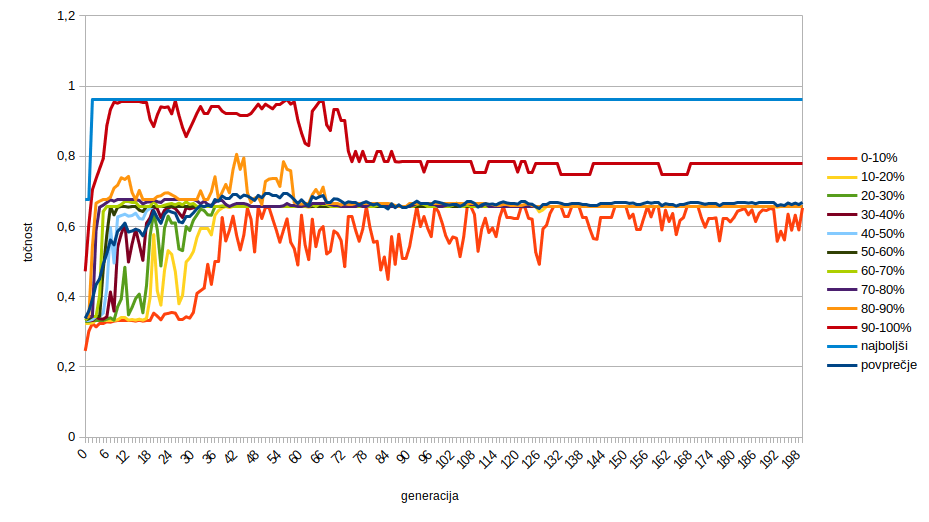
\includegraphics[width=13cm]{iris/1/acc}
    \end{center}
    \caption{Graf točnosti populacije najboljšega agenta prvega nabora skozi generacije.}
    \label{fig:iris_acc_1}
\end{figure}

\begin{figure}[H]
    \begin{center}
        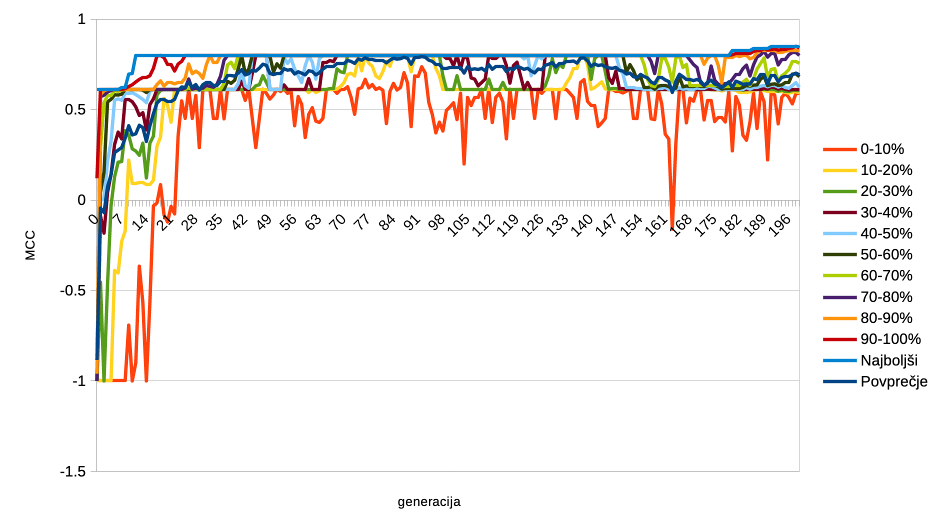
\includegraphics[width=13cm]{iris/1/mcc}
    \end{center}
    \caption{Graf MKK populacije najboljšega agenta prvega nabora skozi generacije.}
    \label{fig:iris_mcc_1}
\end{figure}

\begin{figure}[H]
    \begin{center}
        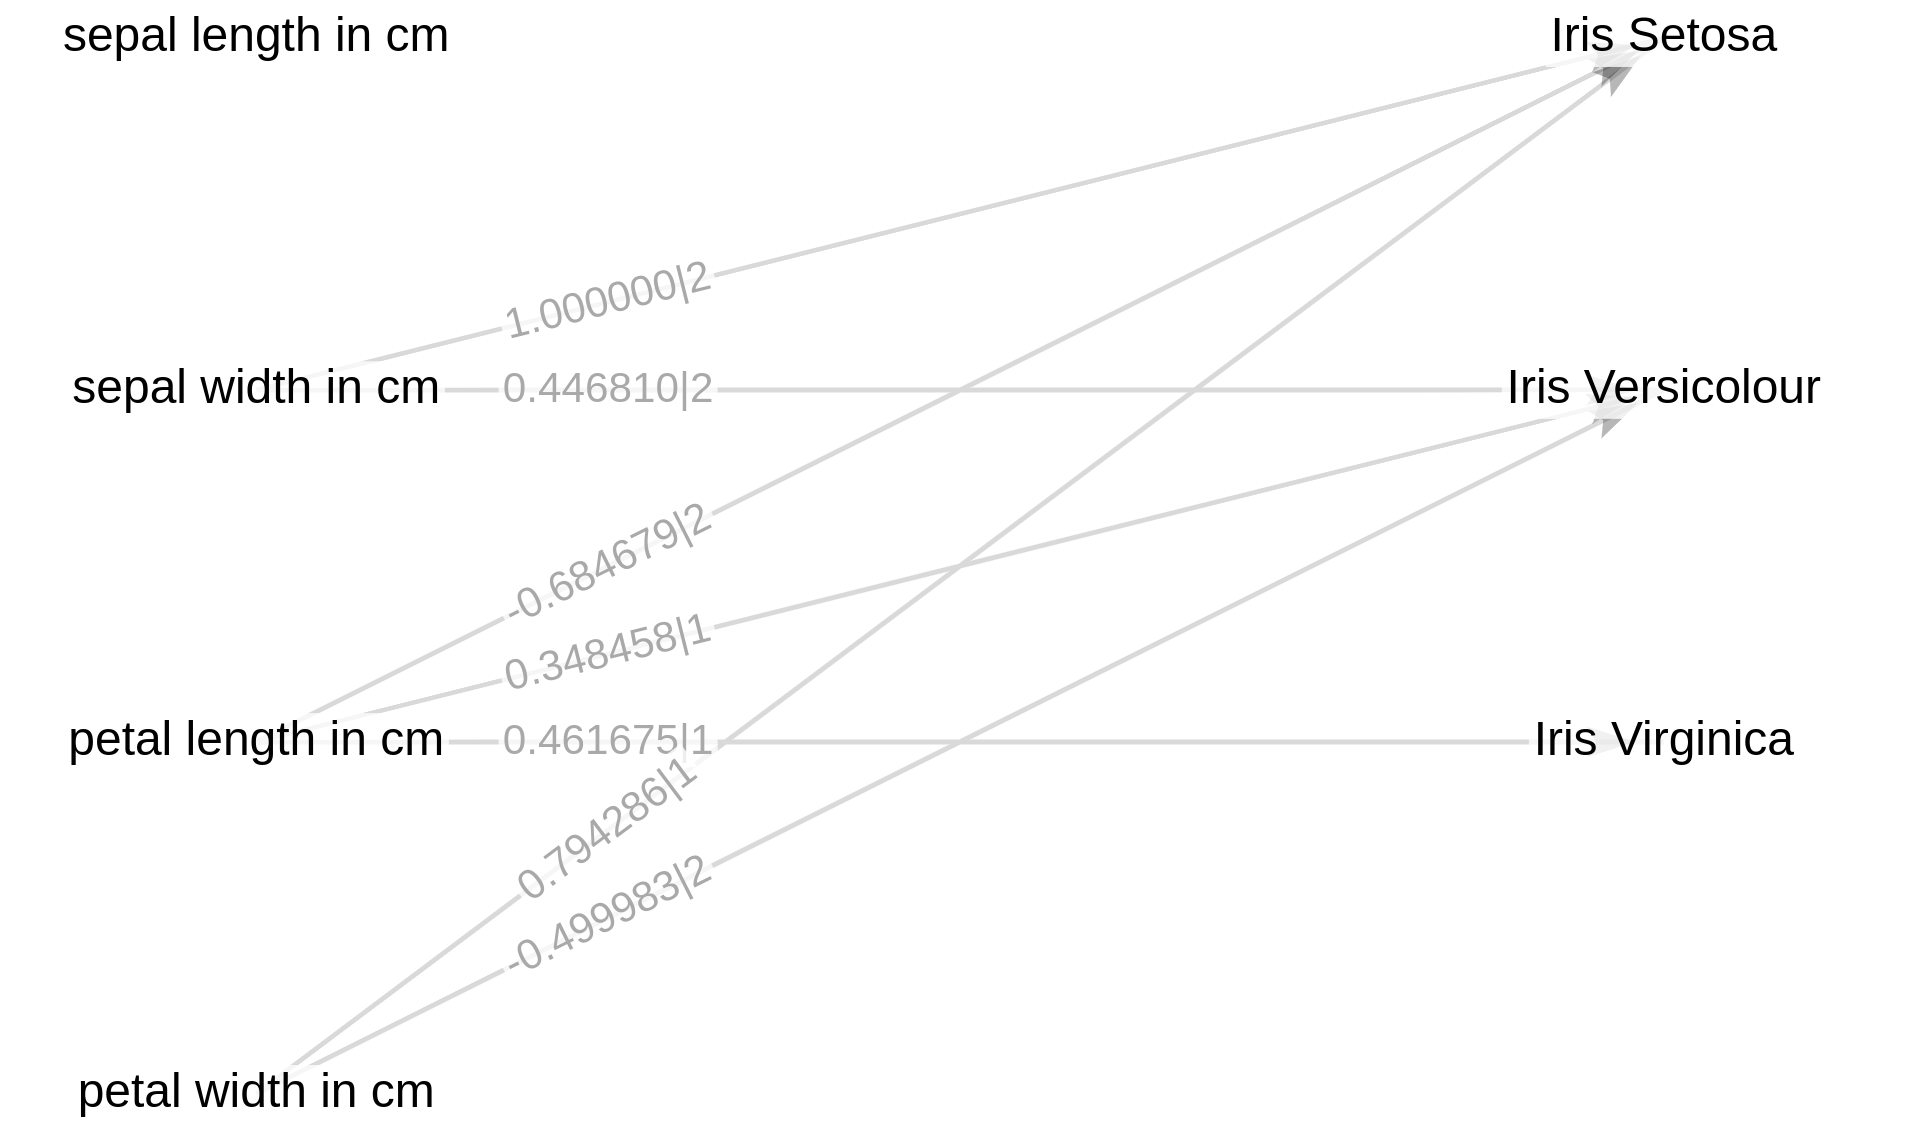
\includegraphics[width=13cm]{iris/1/acc_g}
    \end{center}
    \caption{Vizualizacija najbolj točnega agenta prvega nabora. Vsebuje 5 povezav.}
    \label{fig:iris_acc_1_g}
\end{figure}

\begin{figure}[H]
    \begin{center}
        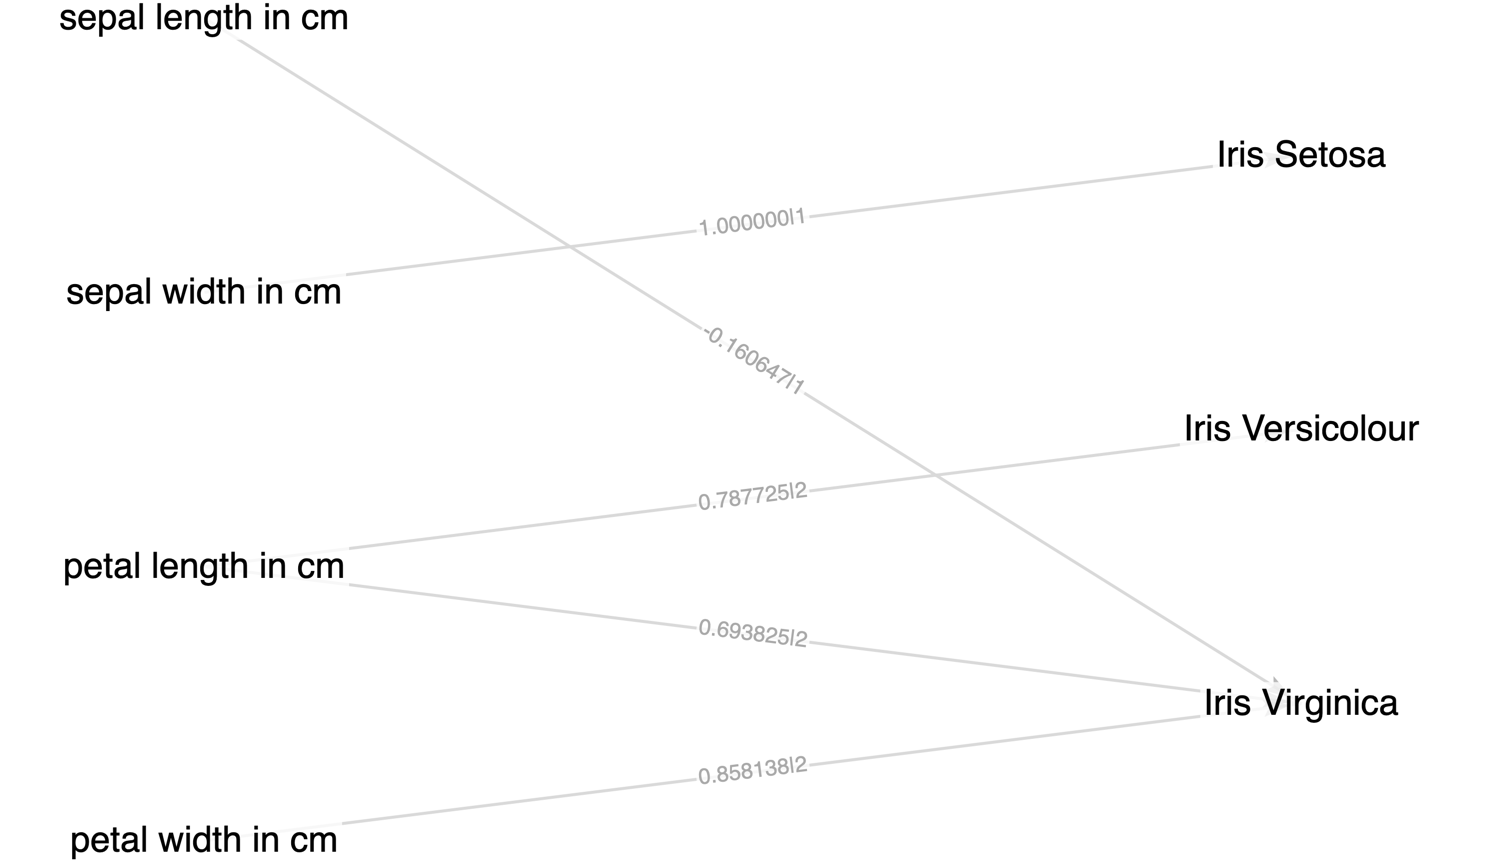
\includegraphics[width=13cm]{iris/1/mcc_g}
    \end{center}
    \caption{Vizualizacija agenta z največjim MKK prvega nabora. Vsebuje 6 povezav.}
    \label{fig:iris_mcc_1_g}
\end{figure}

\newpage

\subsection{Drugi nabor}\label{subsec:dodatek-iris-drugi-nabor}
%%"/home/jure/CLionProjects/Neuroevolution/datasets/iris/iris.data" 150 10 20 2 true 0.1 75 true -0.00001 200 ACC
\begin{table}[H]
    \begin{center}
        \begin{tabular}{|| c | c c || c c ||}
            \hline
            \multirow{2}{*}{št. zagona} & \multicolumn{2}{c||}{točnost najboljšega agenta} & \multicolumn{2}{c||}{MKK najboljšega agenta} \\ \cline{2-5}
            & učna   & testna          & učna  & testna                  \\
            \hline
            1         & 95.2\% & \textbf{97.8\%} & 0.986 & 0.901                   \\
            \hline
            2         & 96.2\% & 95.6\%          & 0.958 & 0.906                   \\
            \hline
            3         & 85.7\% & 93.3\%          & 0.958 & \textbf{0.967 (97.8\%)} \\
            \hline
            4         & 96.2\% & 93.3\%          & 0.986 & 0.902                   \\
            \hline
            5         & 95.2\% & 95.6\%          & 0.945 & 0.906                   \\
            \hline
            povprečje & 93.7\% & 94.7\%          & 0.967 & 0.916                   \\
            \hline
            $\sigma$  & 0.040  & 0.017           & 0.017 & 0.025                   \\
            \hline
        \end{tabular}
    \end{center}
    \caption{Rezultat drugega nabora parametrov.}
    \label{tab:iris_result_2}
\end{table}

\begin{table}[H]
    \centering
    \begin{tabular}{||rcccc||}
        \hline
        razred           & Iris Setosa & Iris Versicolour & Iris Virginica & vsota \\ \hline
        ris Setosa       & 15          & 0                & 0              & 15    \\ \hline
        Iris Versicolour & 0           & 15               & 0              & 15    \\ \hline
        Iris Virginica   & 0           & 1                & 14             & 15    \\ \hline
        vsota            & 15          & 16               & 14             & 45    \\ \hline
    \end{tabular}
    \caption{Matrika zmot najbolj točnega agenta drugega nabora.}
    \label{tab:iris_acc_2}
\end{table}

\begin{table}[H]
    \centering
    \begin{tabular}{||rcccc||}
        \hline
        razred           & Iris Setosa & Iris Versicolour & Iris Virginica & vsota \\ \hline
        ris Setosa       & 15          & 0                & 0              & 15    \\ \hline
        Iris Versicolour & 0           & 14               & 1              & 15    \\ \hline
        Iris Virginica   & 0           & 0                & 15             & 15    \\ \hline
        vsota            & 15          & 14               & 16             & 45    \\ \hline
    \end{tabular}
    \caption{Matrika zmot agenta z največjim MKK drugega nabora.}
    \label{tab:iris_mcc_2}
\end{table}

\begin{figure}[H]
    \begin{center}
        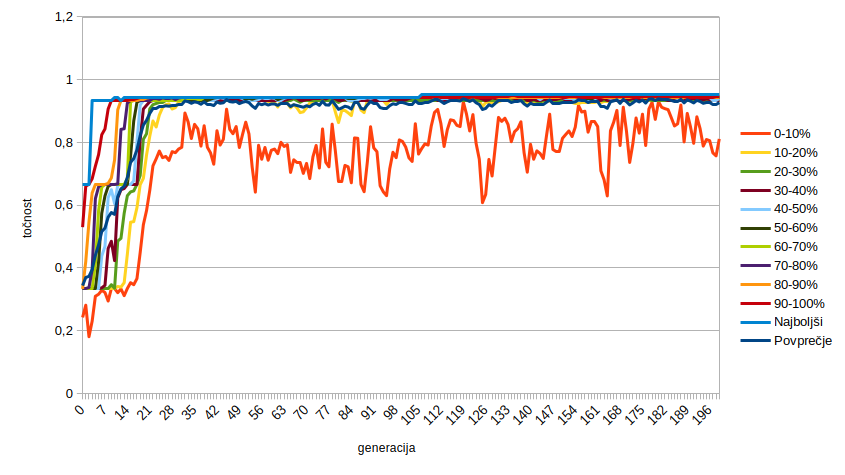
\includegraphics[width=13cm]{iris/2/acc}
    \end{center}
    \caption{Graf točnosti populacije najboljšega agenta drugega nabora skozi generacije.}
    \label{fig:iris_acc_2}
\end{figure}

\begin{figure}[H]
    \begin{center}
        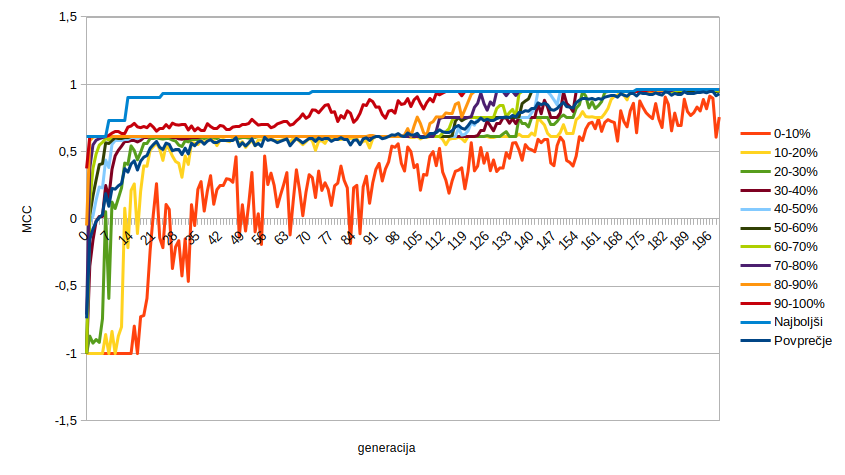
\includegraphics[width=13cm]{iris/2/mcc}
    \end{center}
    \caption{Graf MKK populacije najboljšega agenta drugega nabora skozi generacije.}
    \label{fig:iris_mcc_2}
\end{figure}

\begin{figure}[H]
    \begin{center}
        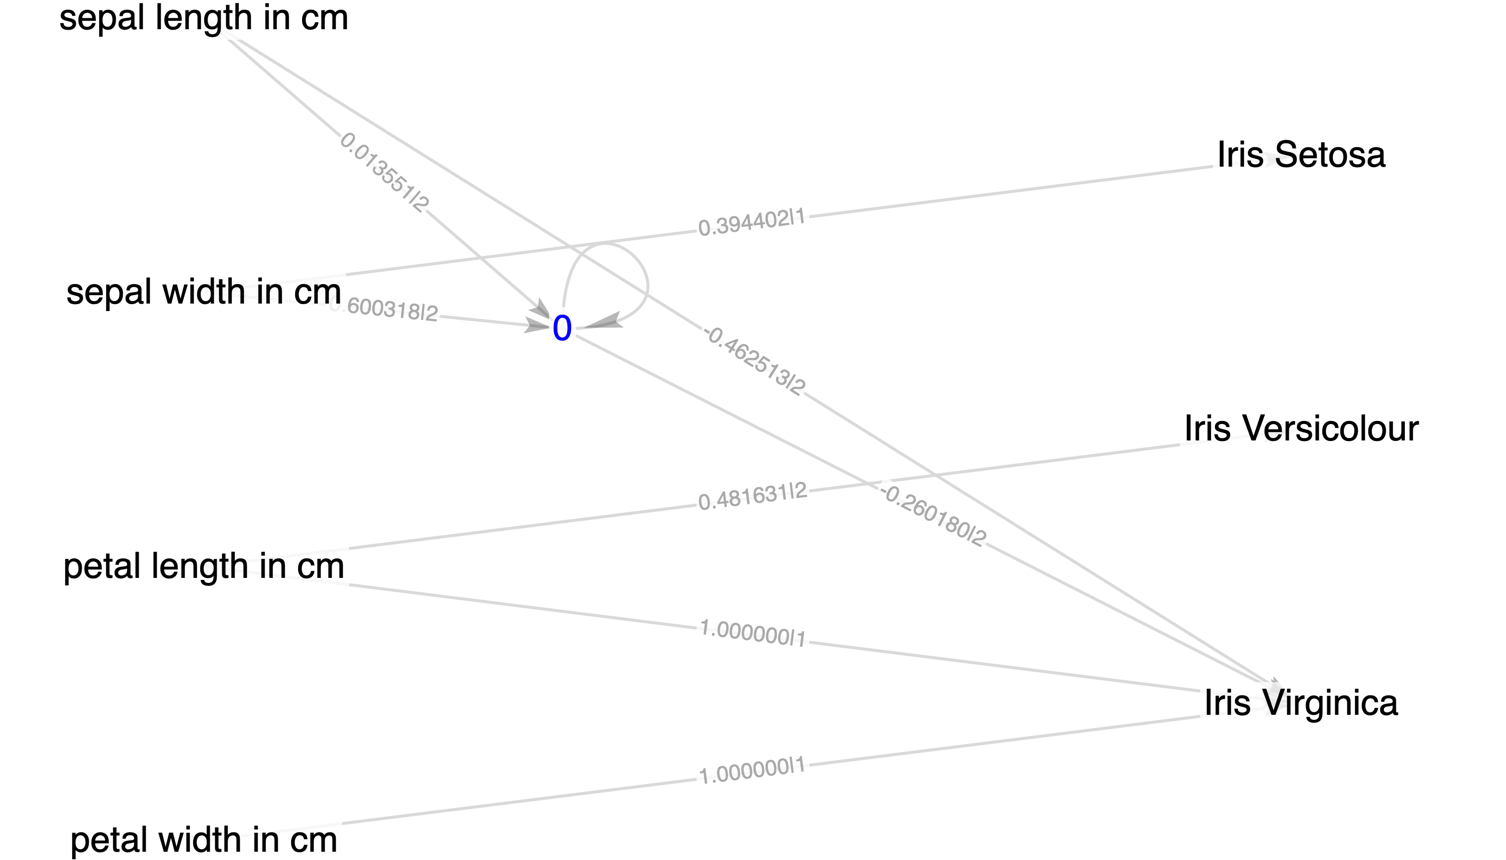
\includegraphics[width=13cm]{iris/2/acc_g}
    \end{center}
    \caption{Vizualizacija najbolj točnega agenta drugega nabora. Vsebuje 2 vmesni vozlišči in 8 povezav.}
    \label{fig:iris_acc_2_g}
\end{figure}

\begin{figure}[H]
    \begin{center}
        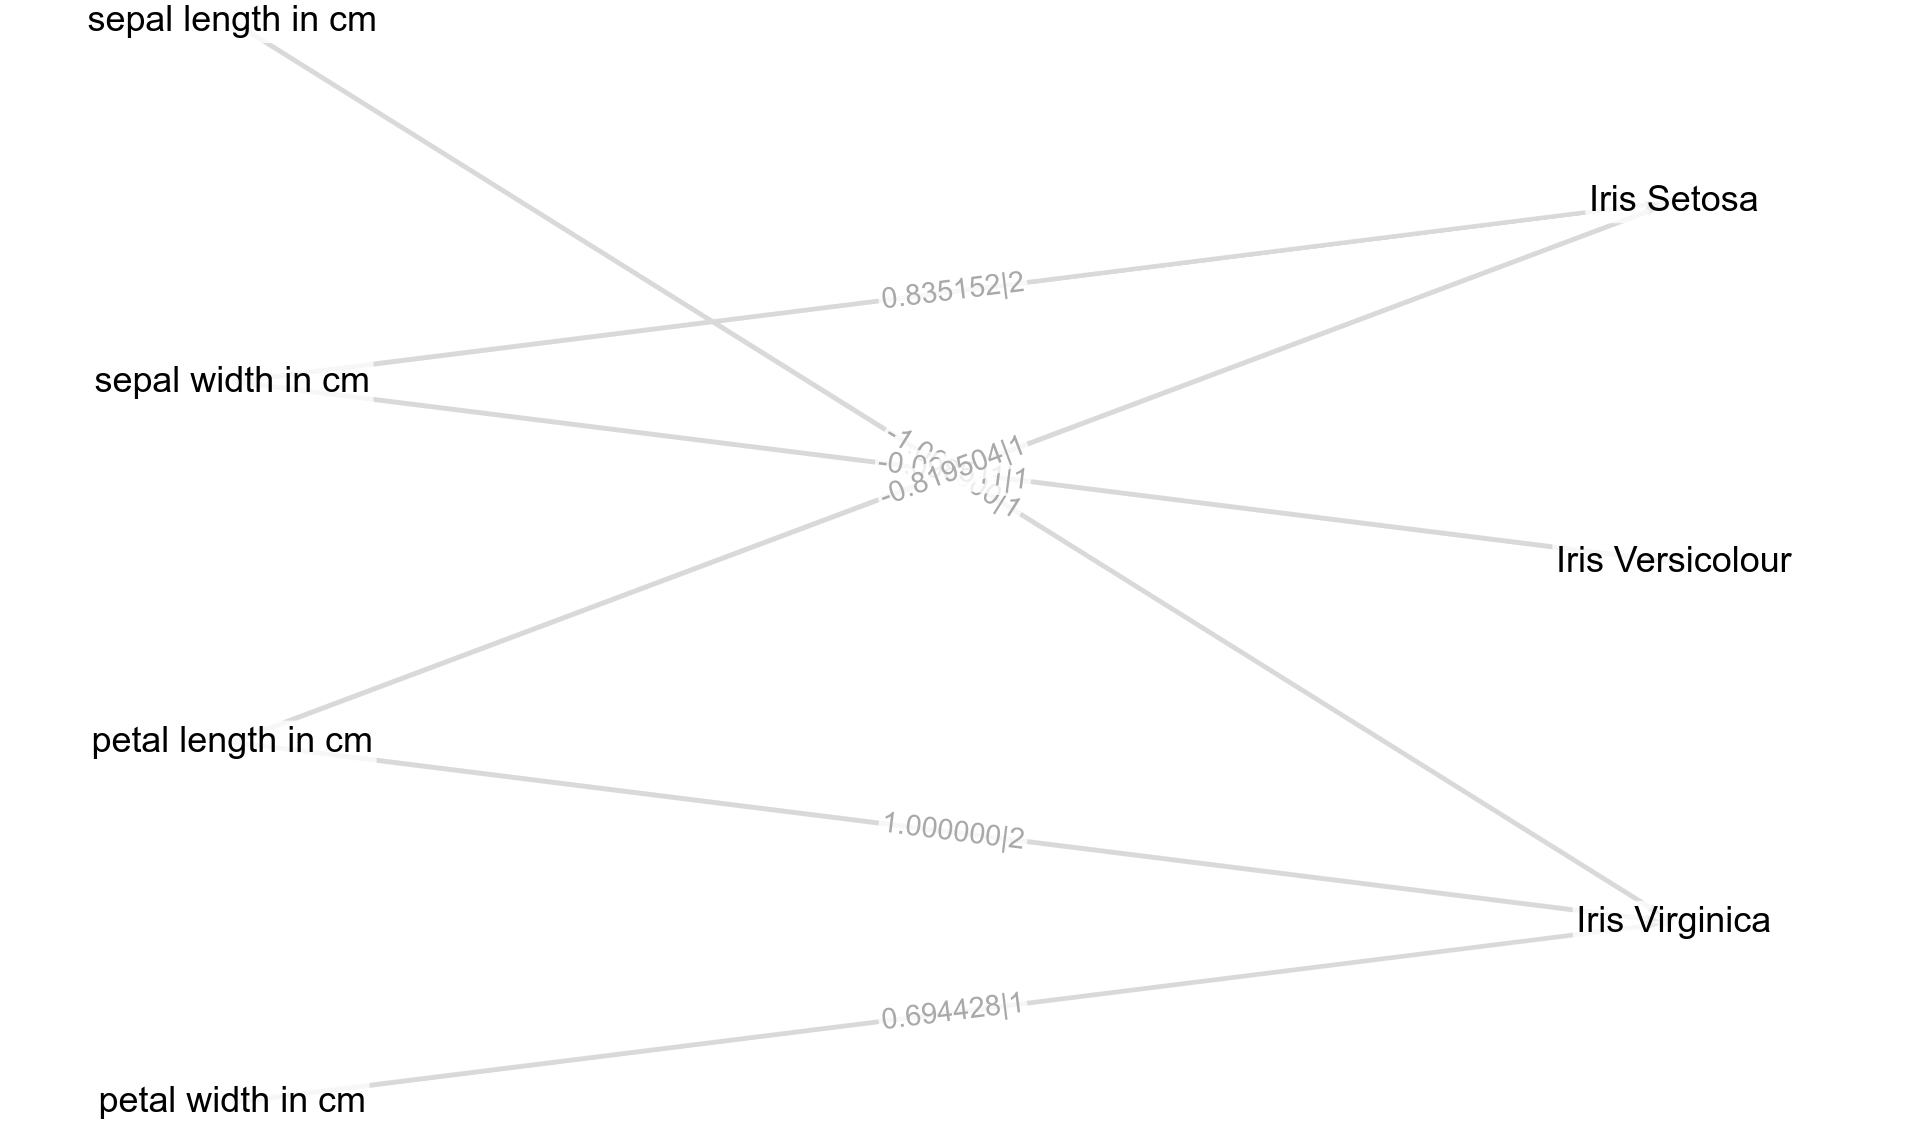
\includegraphics[width=13cm]{iris/2/mcc_g}
    \end{center}
    \caption{Vizualizacija agenta z največjim MKK drugega nabora. Vsebuje 6 povezav.}
    \label{fig:iris_mcc_2_g}
\end{figure}

\subsection{Tretji nabor}\label{subsec:dodatek-iris-tretji-nabor}
%%"/home/jure/CLionProjects/Neuroevolution/datasets/iris/iris.data" 200 15 30 3 true 0.1 100 true -0.00001 300 ACC
\begin{table}[H]
    \begin{center}
        \begin{tabular}{|| c | c c || c c ||}
            \hline
            \multirow{2}{*}{št. zagona} & \multicolumn{2}{c||}{točnost najboljšega agenta} & \multicolumn{2}{c||}{MKK najboljšega agenta} \\ \cline{2-5}
            & učna   & testna          & učna  & testna                  \\
            \hline
            1         & 97.1\% & 95.6\%          & 0.958 & 0.849                   \\
            \hline
            2         & 89.5\% & 75.6\%          & 0.945 & \textbf{0.936 (95.6\%)} \\
            \hline
            3         & 97.1\% & 93.3\%          & 0.972 & 0.834                   \\
            \hline
            4         & 95.2\% & \textbf{97.8\%} & 0.972 & 0.934                   \\
            \hline
            5         & 97.1\% & 97.8\%          & 0.972 & 0.936                   \\
            \hline
            povprečje & 95.2\% & 92.0\%          & 0.964 & 0.898                   \\
            \hline
            $\sigma$  & 0.029  & 0.084           & 0.011 & 0.046                   \\
            \hline
        \end{tabular}
    \end{center}
    \caption{Rezultat tretjega nabora parametrov.}
    \label{tab:iris_result_3}
\end{table}

\begin{table}[H]
    \centering
    \begin{tabular}{||rcccc||}
        \hline
        razred           & Iris Setosa & Iris Versicolour & Iris Virginica & vsota \\ \hline
        ris Setosa       & 14          & 1                & 0              & 15    \\ \hline
        Iris Versicolour & 0           & 15               & 0              & 15    \\ \hline
        Iris Virginica   & 0           & 0                & 15             & 15    \\ \hline
        vsota            & 14          & 15               & 15             & 45    \\ \hline
    \end{tabular}
    \caption{Matrika zmot najbolj točnega agenta tretjega nabora.}
    \label{tab:iris_acc_3}
\end{table}

\begin{table}[H]
    \centering
    \begin{tabular}{||rcccc||}
        \hline
        razred           & Iris Setosa & Iris Versicolour & Iris Virginica & vsota \\ \hline
        ris Setosa       & 15          & 0                & 0              & 15    \\ \hline
        Iris Versicolour & 0           & 13               & 2              & 15    \\ \hline
        Iris Virginica   & 0           & 0                & 15             & 15    \\ \hline
        vsota            & 15          & 13               & 17             & 45    \\ \hline
    \end{tabular}
    \caption{Matrika zmot agenta z največjim MKK tretjega nabora.}
    \label{tab:iris_mcc_3}
\end{table}

\begin{figure}[H]
    \begin{center}
        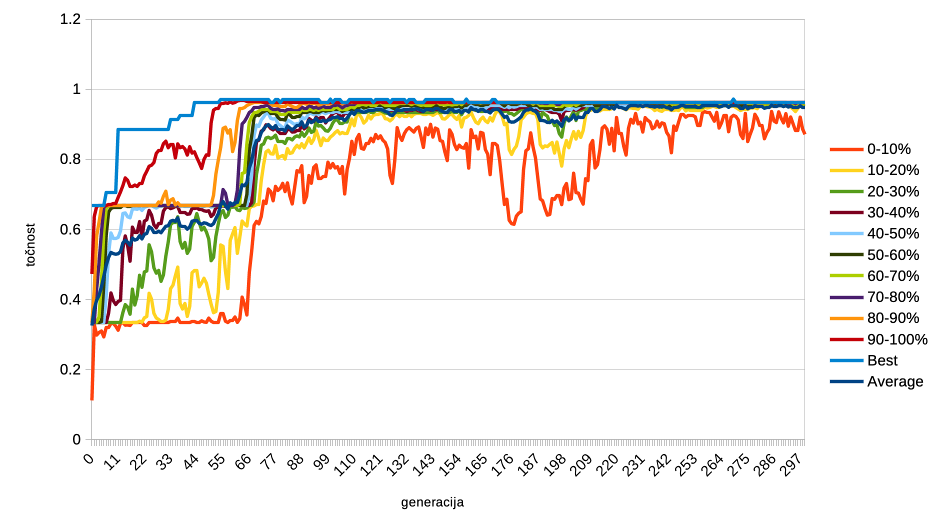
\includegraphics[width=13cm]{iris/3/acc}
    \end{center}
    \caption{Graf točnosti populacije najboljšega agenta tretjega nabora skozi generacije.}
    \label{fig:iris_acc_3}
\end{figure}

\begin{figure}[H]
    \begin{center}
        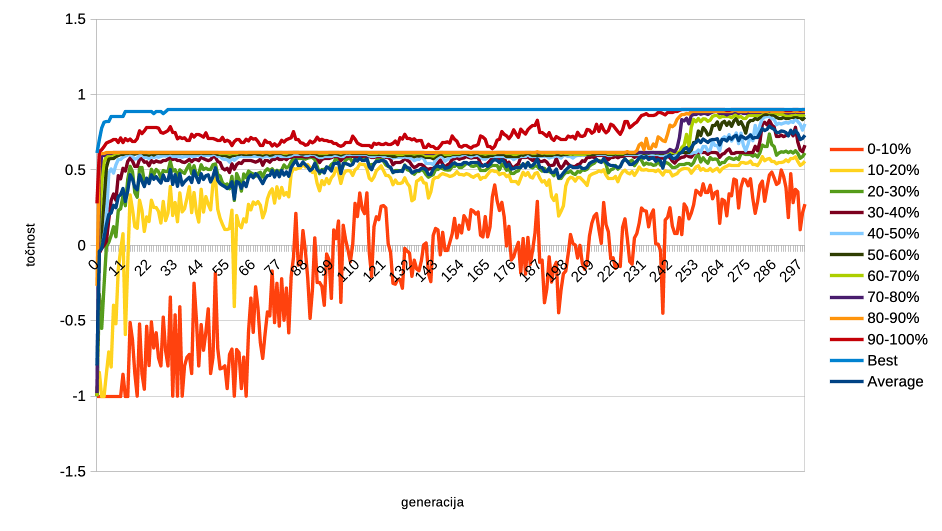
\includegraphics[width=13cm]{iris/3/mcc}
    \end{center}
    \caption{Graf MKK populacije najboljšega agenta tretjega nabora skozi generacije.}
    \label{fig:iris_mcc_3}
\end{figure}

\begin{figure}[H]
    \begin{center}
        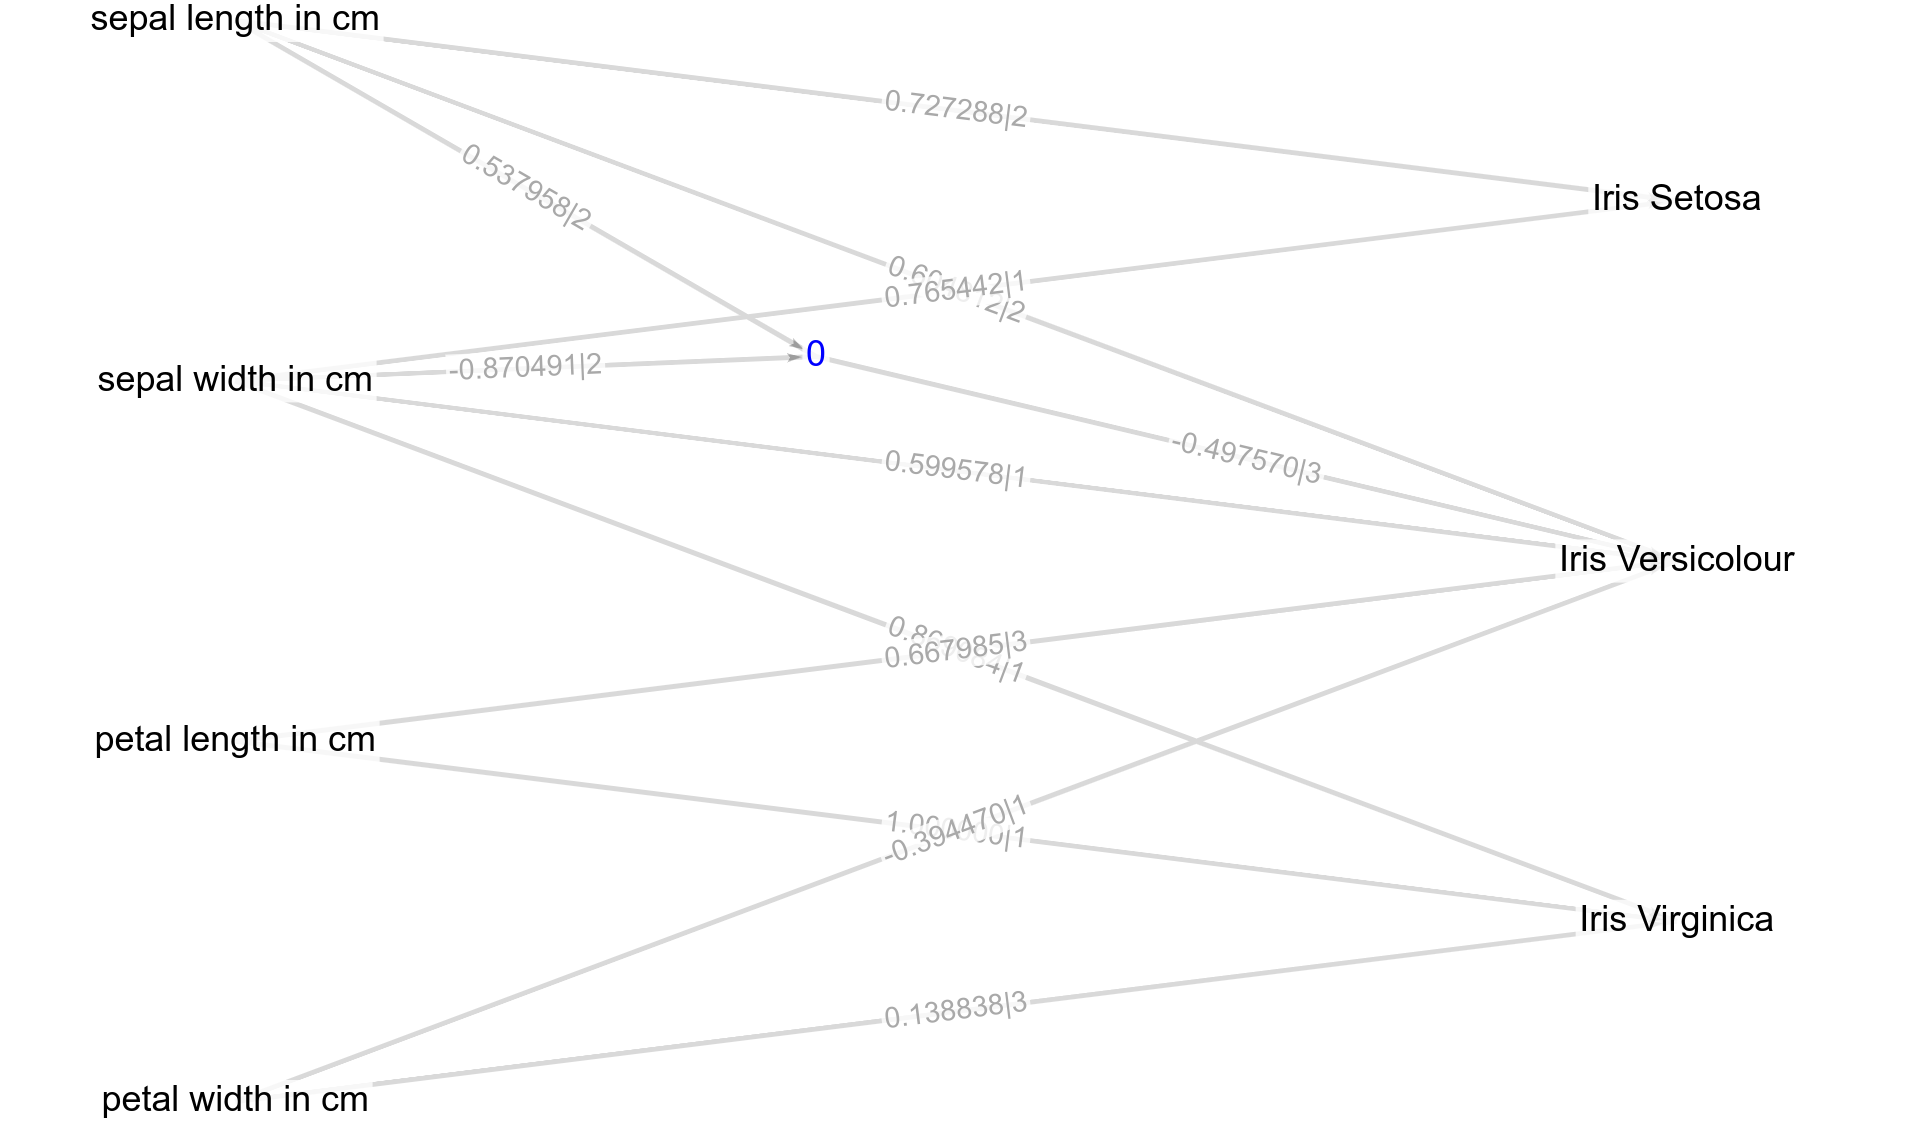
\includegraphics[width=13cm]{iris/3/acc_g}
    \end{center}
    \caption{Vizualizacija najbolj točnega agenta tretjega nabora. Vsebuje 1 vmesno vozlišče in 12 povezav.}
    \label{fig:iris_acc_3_g}
\end{figure}

\begin{figure}[H]
    \begin{center}
        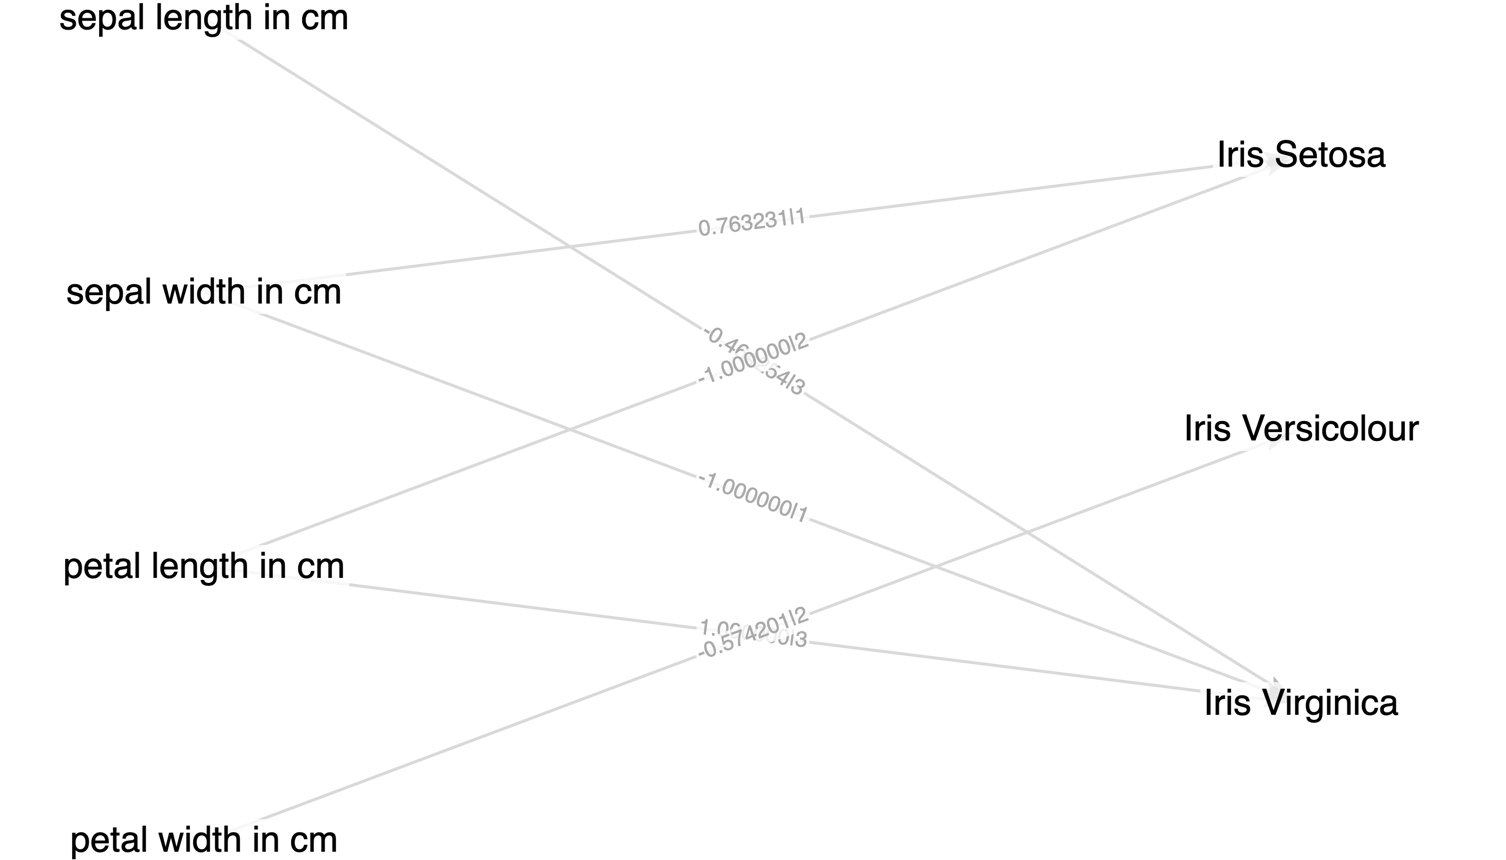
\includegraphics[width=13cm]{iris/3/mcc_g}
    \end{center}
    \caption{Vizualizacija agenta z največjim MKK drugega nabora. Vsebuje 1 vmesno vozlišče in 9 povezav.}
    \label{fig:iris_mcc_3_g}
\end{figure}

\section{Wine}\label{sec:dodatek-wine-test}
%% arrowLength=20
%% linkWidth=2
%% input fy=50*node.pos
%% output fx=700
%% output fy=150*node.pos+120
%% MAX_FONT_SIZE=12
\begin{table}[H]
    \begin{center}
        \begin{tabular}{||l c c c||}
            \hline
            & 1      & 2      & 3 \\ [0.5ex]
            \hline
            velikost populacije               & 200    & 250    & 350    \\
            \hline
            največje število globokih vozlišč & 15     & 20     & 25     \\
            \hline
            največje število povezav          & 30     & 50     & 75     \\
            \hline
            največje število prečkanj         & 2      & 3      & 4      \\
            \hline
            delež mutiranih potomcev          & 10\%   & 10\%   & 10\%   \\
            \hline
            prispevek vozlišč                 & -0.001 & -0.001 & -0.001 \\
            \hline
            prispevek povezav                 & -0.001 & -0.001 & -0.001 \\
            \hline
            število generacij                 & 300    & 350    & 450    \\
            \hline
        \end{tabular}
    \end{center}
    \caption{Nabori inicializacijskih parametrov poganjanja na množici Wine.}
    \label{tab:param_wine}
\end{table}

\subsection{Prvi nabor}\label{subsec:dodatek-wine-prvi-nabor}
%%"/home/jure/CLionProjects/Neuroevolution/datasets/wine/wine.data" 200 15 30 2 true 0.1 100 true -0.001 -0.001 300 ACC
\begin{table}[H]
    \begin{center}
        \begin{tabular}{|| c | c c || c c ||}
            \hline
            \multirow{2}{*}{št. zagona} & \multicolumn{2}{c||}{točnost najboljšega agenta} & \multicolumn{2}{c||}{MCC najboljšega agenta} \\ \cline{2-5}
            & učna   & testna          & učna  & testna                  \\
            \hline
            1        & 92.0\% & 75.5\%          & 0.868 & \textbf{0.918 (94.3\%)} \\
            \hline
            2        & 94.4\% & 92.5\%          & 0.808 & 0.843                   \\
            \hline
            3        & 92.0\% & 92.5\%          & 0.818 & 0.779                   \\
            \hline
            4        & 96.8\% & \textbf{94.3\%} & 0.820 & 0.677                   \\
            \hline
            5        & 84.8\% & 75.5\%          & 0.904 & 0.830                   \\
            \hline
            $\sigma$ & 0.040  & 0.086           & 0.037 & 0.08                    \\
            \hline
        \end{tabular}
    \end{center}
    \caption{Rezultat prvega nabora parametrov.}
    \label{tab:wine_result_1}
\end{table}

\begin{table}[H]
    \centering
    \begin{tabular}{||rcccc||}
        \hline
        razred  & Class 1 & Class 2 & Class 3 & vsota \\ \hline
        Class 1 & 17      & 1       & 0       & 18    \\ \hline
        Class 2 & 2       & 19      & 0       & 21    \\ \hline
        Class 3 & 0       & 0       & 14      & 14    \\ \hline
        vsota   & 19      & 20      & 14      & 53    \\ \hline
    \end{tabular}
    \caption{Matrika zmot najbolj točnega agenta prvega nabora.}
    \label{tab:wine_acc_1}
\end{table}

\begin{table}[H]
    \centering
    \begin{tabular}{||rcccc||}
        \hline
        razred  & Class 1 & Class 2 & Class 3 & vsota \\ \hline
        Class 1 & 18      & 0       & 0       & 18    \\ \hline
        Class 2 & 2       & 18      & 1       & 21    \\ \hline
        Class 3 & 0       & 0       & 14      & 14    \\ \hline
        vsota   & 20      & 18      & 15      & 53    \\ \hline
    \end{tabular}
    \caption{Matrika zmot agenta z največjim MCC prvega nabora.}
    \label{tab:wine_mcc_1}
\end{table}

\begin{figure}[H]
    \begin{center}
        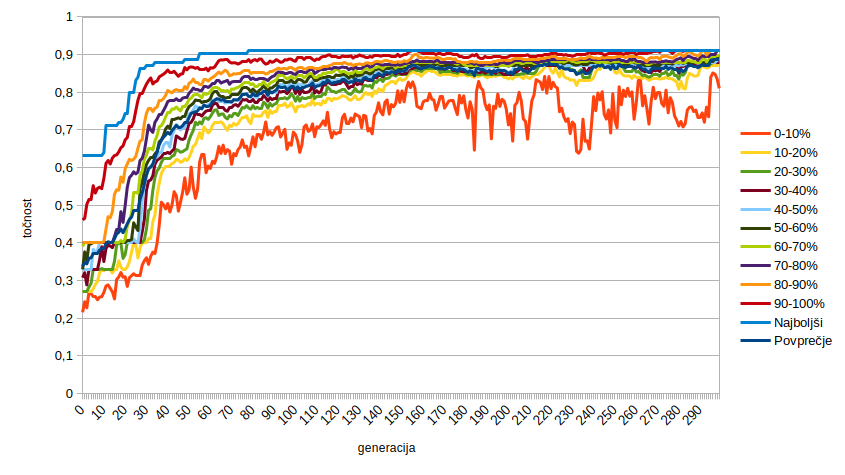
\includegraphics[width=13cm]{wine/1/acc}
    \end{center}
    \caption{Graf točnosti populacije najboljšega agenta prvega nabora skozi generacije.}
    \label{fig:wine_acc_1}
\end{figure}

\begin{figure}[H]
    \begin{center}
        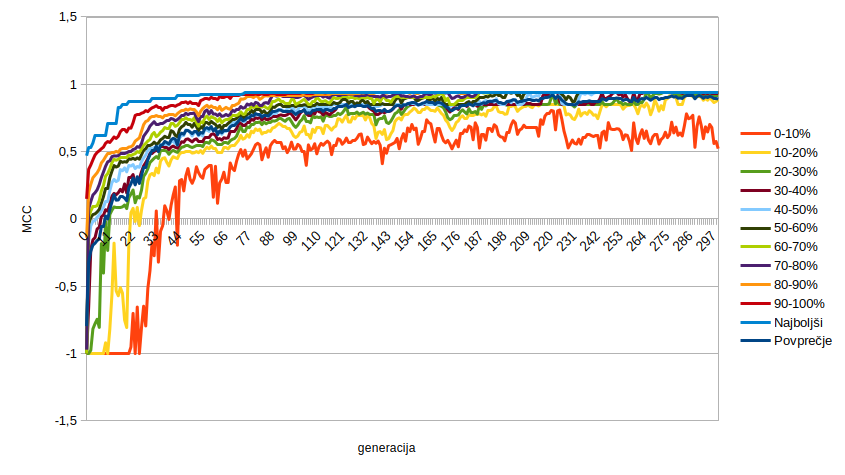
\includegraphics[width=13cm]{wine/1/mcc}
    \end{center}
    \caption{Graf MCC populacije najboljšega agenta prvega nabora skozi generacije.}
    \label{fig:wine_mcc_1}
\end{figure}

\begin{figure}[H]
    \begin{center}
        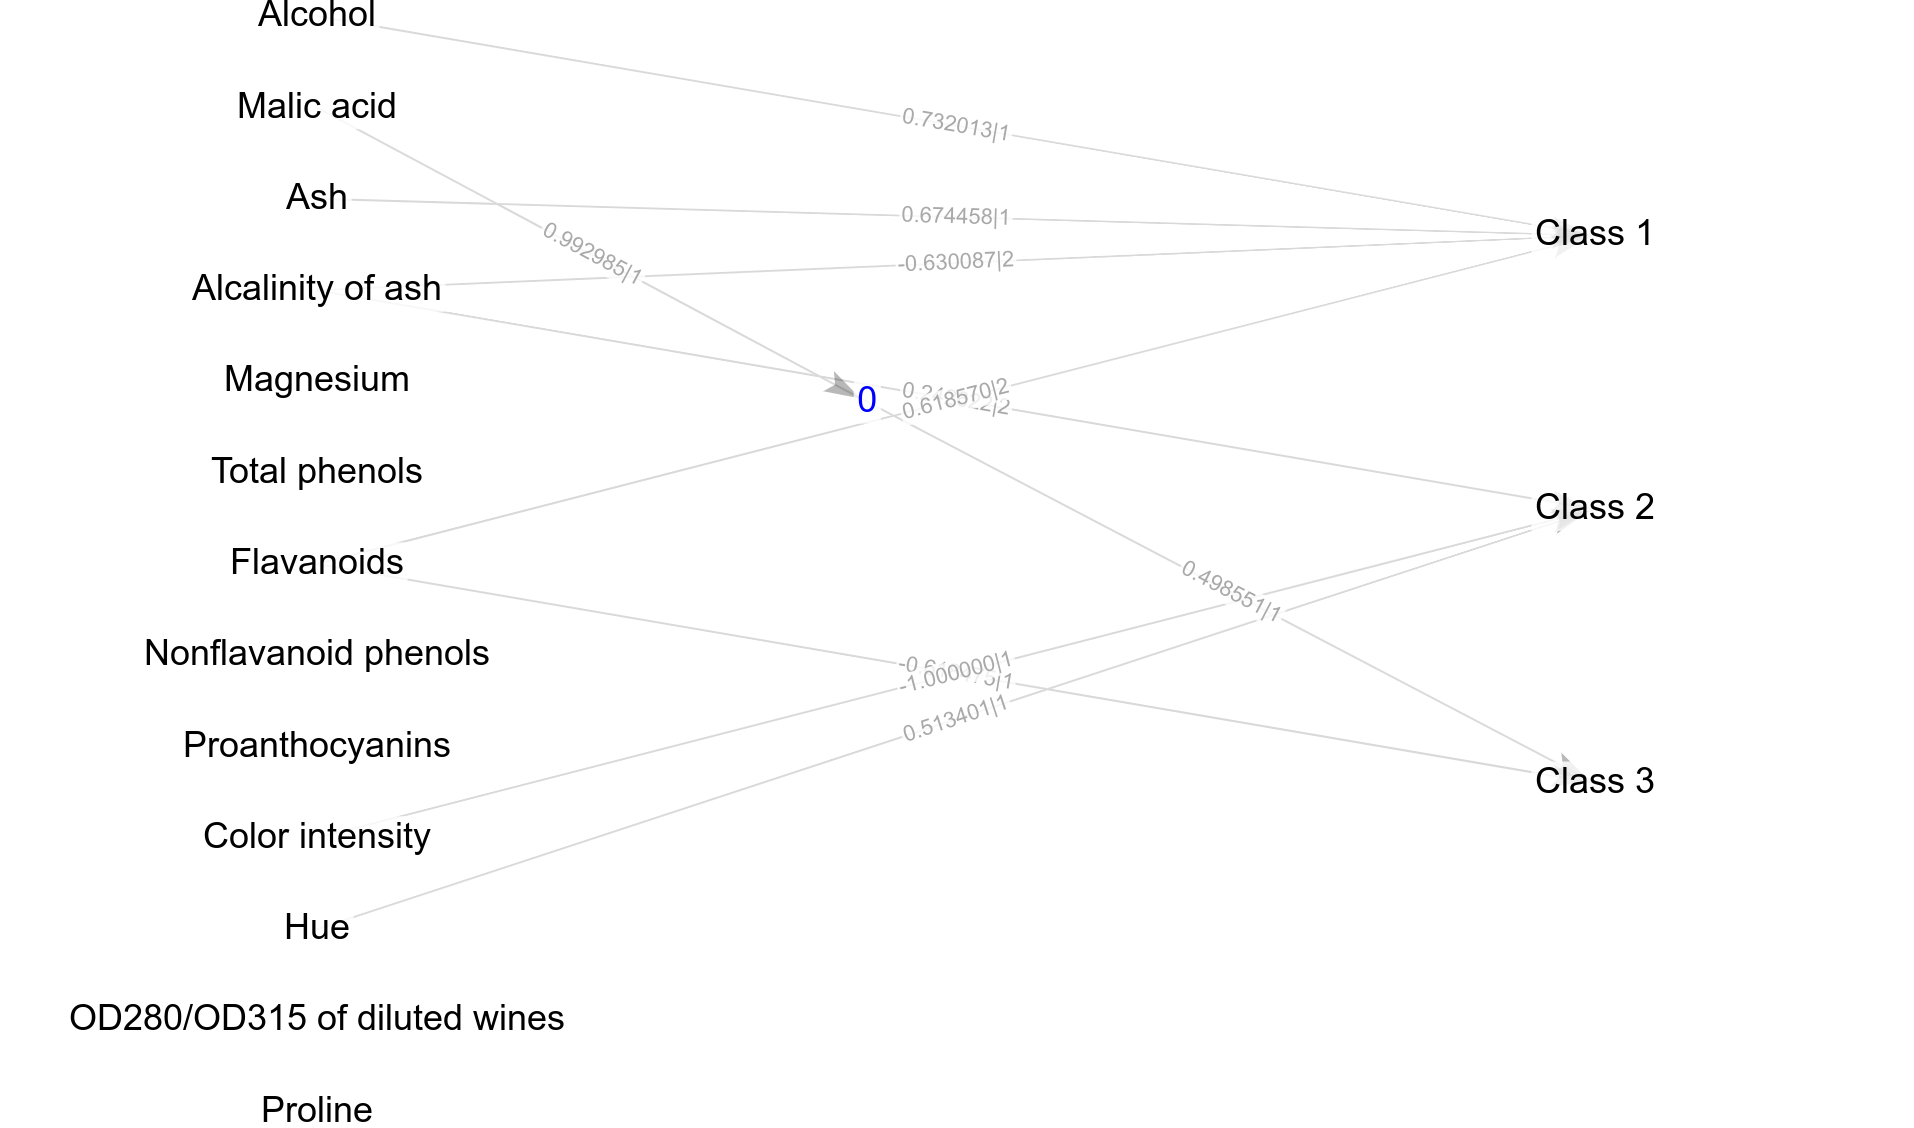
\includegraphics[width=13cm]{wine/1/acc_g}
    \end{center}
    \caption{Vizualizacija najbolj točnega agenta prvega nabora. Vsebuje 1 globoko vozlišče in 9 povezav.}
    \label{fig:wine_acc_1_g}
\end{figure}

\begin{figure}[H]
    \begin{center}
        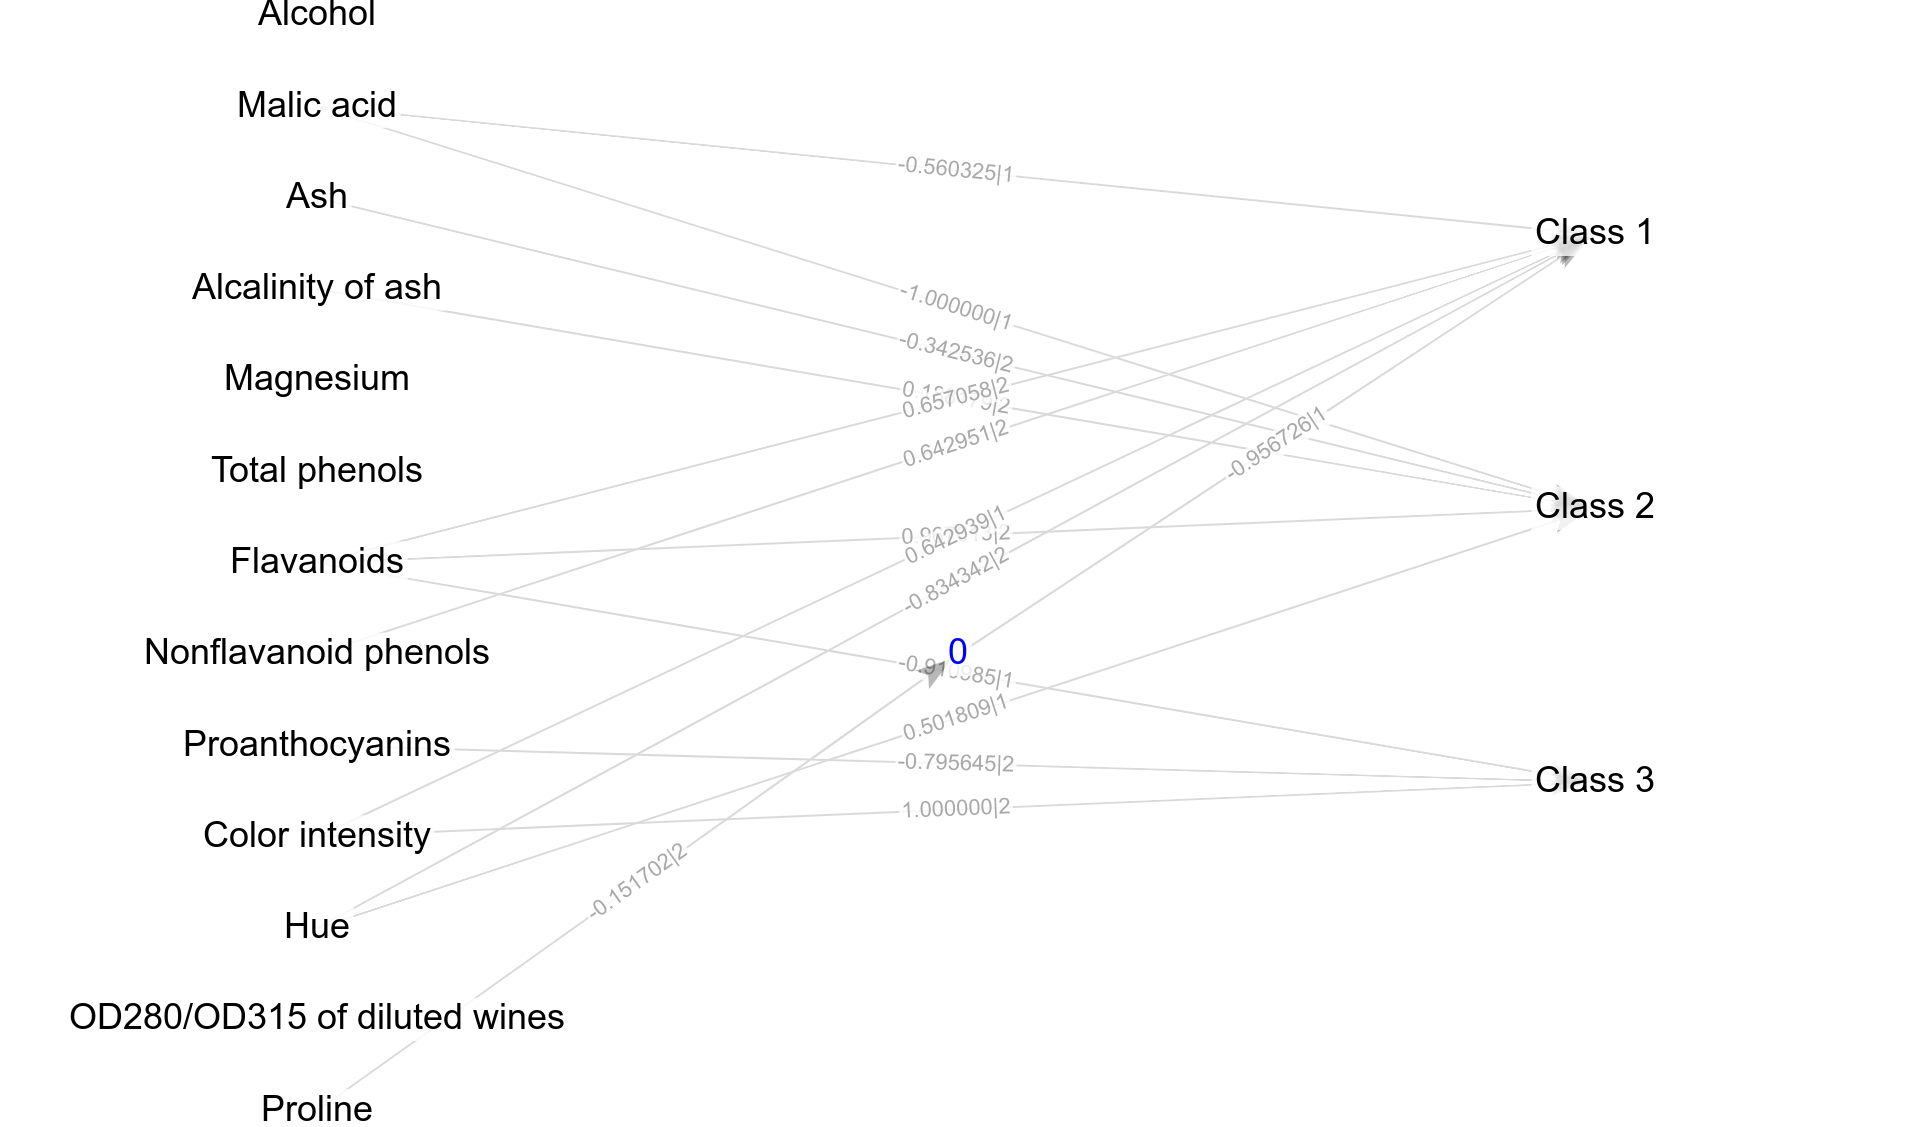
\includegraphics[width=13cm]{wine/1/mcc_g}
    \end{center}
    \caption{Vizualizacija agenta z največjim MCC prvega nabora. Vsebuje 6 povezav.}
    \label{fig:wine_mcc_1_g}
\end{figure}

\subsection{Drugi nabor}\label{subsec:dodatek-wine-drugi-nabor}
%%"/home/jure/CLionProjects/Neuroevolution/datasets/iris/iris.data" 250 20 50 3 true 0.1 100 true -0.001 -0.001 350 ACC
\begin{table}[H]
    \begin{center}
        \begin{tabular}{|| c | c c || c c ||}
            \hline
            \multirow{2}{*}{št. zagona} & \multicolumn{2}{c||}{točnost najboljšega agenta} & \multicolumn{2}{c||}{MCC najboljšega agenta} \\ \cline{2-5}
            & učna   & testna          & učna  & testna                  \\
            \hline
            1        & 83.2\% & 81.1\%          & 0.845 & 0.610                   \\
            \hline
            2        & 67.2\% & 60.4\%          & 0.867 & 0.779                   \\
            \hline
            3        & 76.8\% & 77.4\%          & 0.830 & 0.740                   \\
            \hline
            4        & 92.0\% & \textbf{96.2\%} & 0.915 & \textbf{0.915 (94.3\%)} \\
            \hline
            5        & 93.6\% & 96.2\%          & 0.892 & 0.914                   \\
            \hline
            $\sigma$ & 0.098  & 0.134           & 0.031 & 0.115                   \\
            \hline
        \end{tabular}
    \end{center}
    \caption{Rezultat drugega nabora parametrov.}
    \label{tab:wine_result_2}
\end{table}

\begin{table}[H]
    \centering
    \begin{tabular}{||rcccc||}
        \hline
        razred  & Class 1 & Class 2 & Class 3 & vsota \\ \hline
        Class 1 & 17      & 1       & 0       & 18    \\ \hline
        Class 2 & 0       & 20      & 1       & 21    \\ \hline
        Class 3 & 0       & 0       & 14      & 14    \\ \hline
        vsota   & 17      & 21      & 15      & 53    \\ \hline
    \end{tabular}
    \caption{Matrika zmot najbolj točnega agenta drugega nabora.}
    \label{tab:wine_acc_2}
\end{table}

\begin{table}[H]
    \centering
    \begin{tabular}{||rcccc||}
        \hline
        razred  & Class 1 & Class 2 & Class 3 & vsota \\ \hline
        Class 1 & 17      & 1       & 0       & 18    \\ \hline
        Class 2 & 2       & 19      & 0       & 21    \\ \hline
        Class 3 & 0       & 0       & 14      & 14    \\ \hline
        vsota   & 19      & 20      & 14      & 53    \\ \hline
    \end{tabular}
    \caption{Matrika zmot agenta z največjim MCC drugega nabora.}
    \label{tab:wine_mcc_2}
\end{table}

\begin{figure}[H]
    \begin{center}
        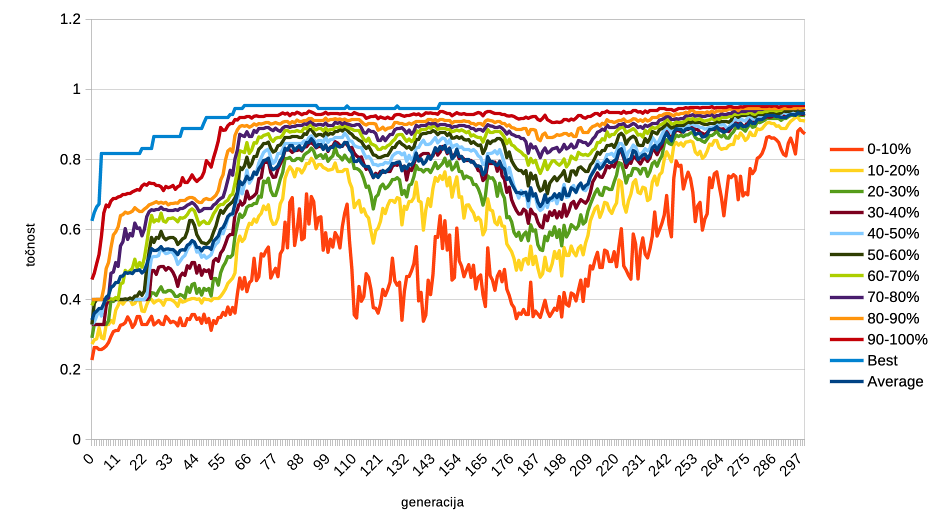
\includegraphics[width=13cm]{wine/2/acc}
    \end{center}
    \caption{Graf točnosti populacije najboljšega agenta drugega nabora skozi generacije.}
    \label{fig:wine_acc_2}
\end{figure}

\begin{figure}[H]
    \begin{center}
        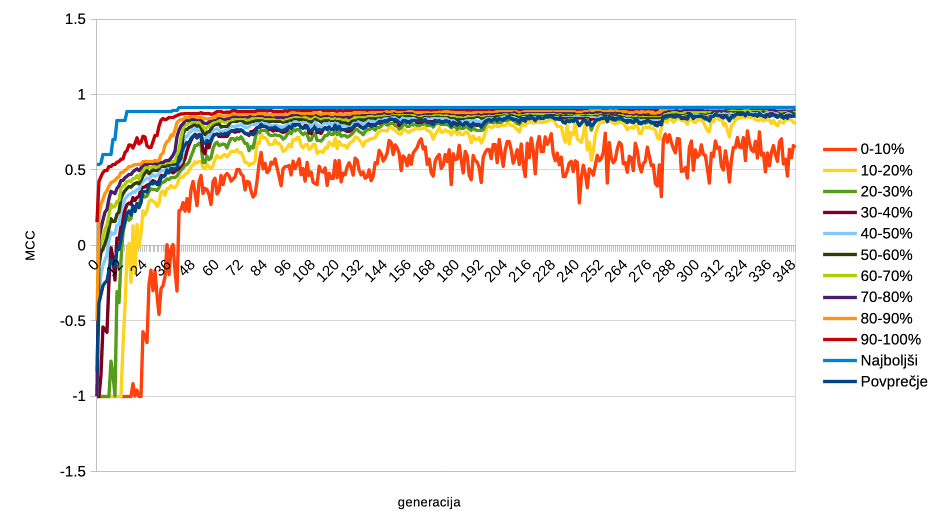
\includegraphics[width=13cm]{wine/2/mcc}
    \end{center}
    \caption{Graf MCC populacije najboljšega agenta drugega nabora skozi generacije.}
    \label{fig:wine_mcc_2}
\end{figure}

\begin{figure}[H]
    \begin{center}
        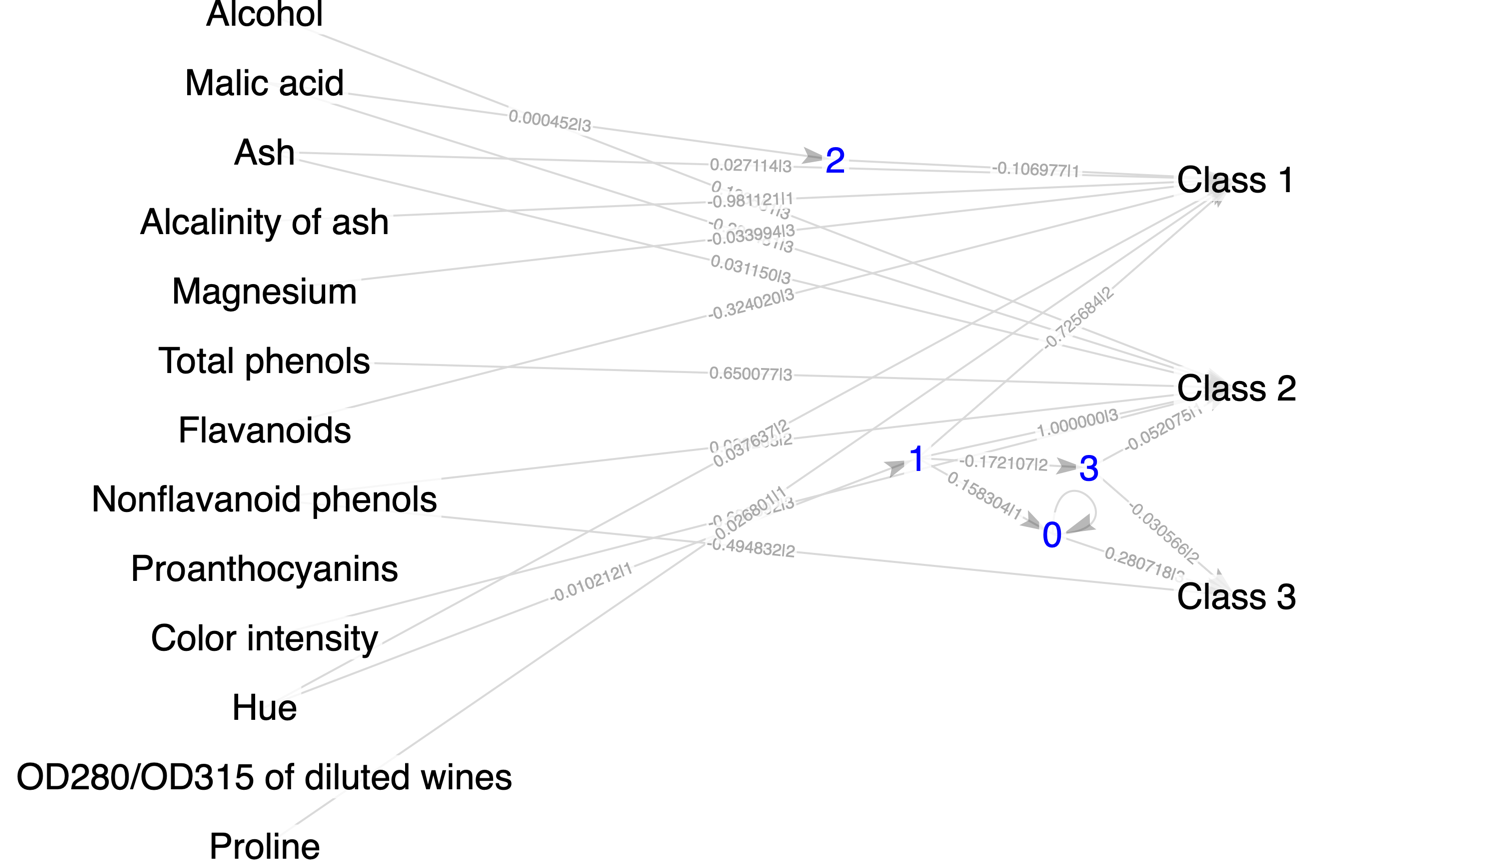
\includegraphics[width=13cm]{wine/2/acc_g}
    \end{center}
    \caption{Vizualizacija najbolj točnega agenta drugega nabora. Vsebuje 6 povezav.}
    \label{fig:wine_acc_2_g}
\end{figure}

\begin{figure}[H]
    \begin{center}
        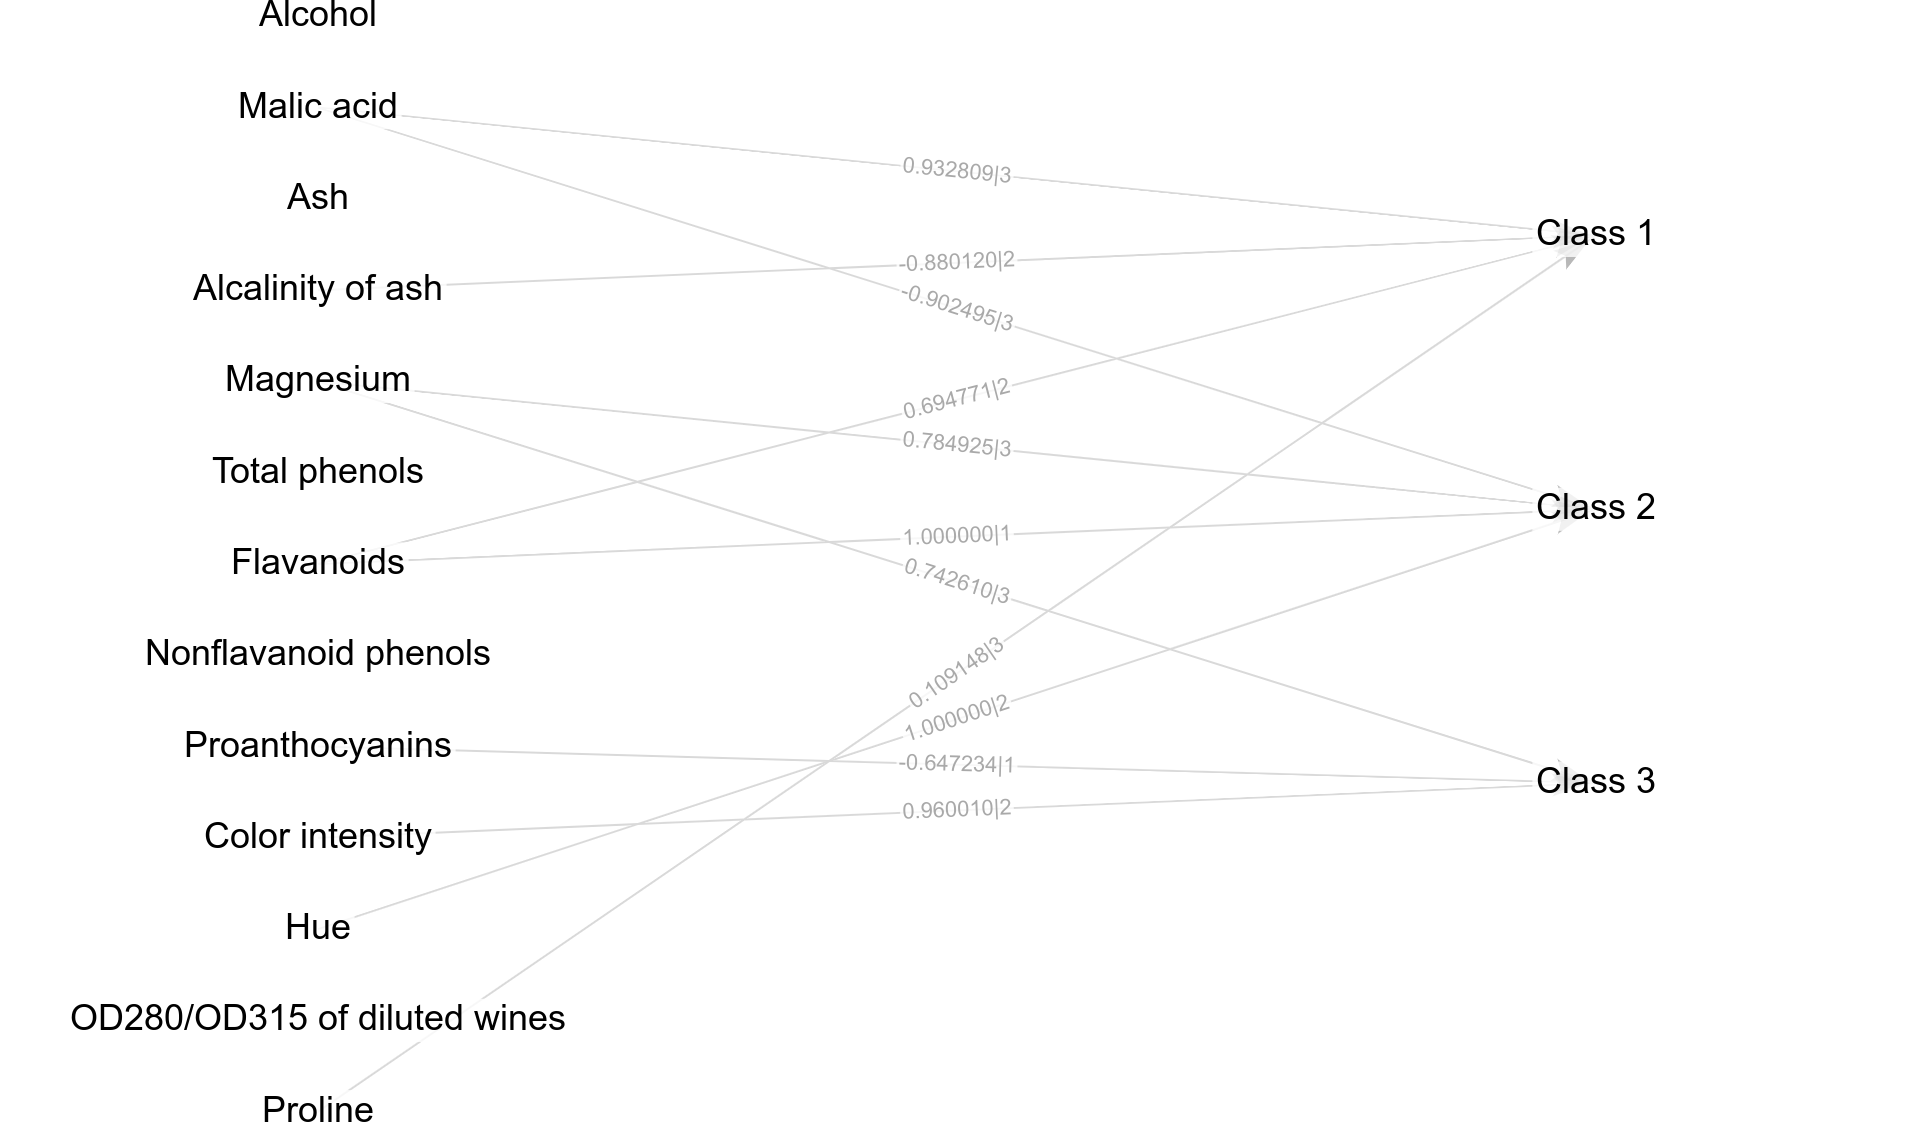
\includegraphics[width=13cm]{wine/2/mcc_g}
    \end{center}
    \caption{Vizualizacija agenta z največjim MCC drugega nabora. Vsebuje 1 globoko vozlišče in 7 povezav.}
    \label{fig:wine_mcc_2_g}
\end{figure}

\subsection{Tretji nabor}\label{subsec:dodatek-wine-tretji-nabor}
%%"/home/jure/CLionProjects/Neuroevolution/datasets/iris/iris.data" 350 25 75 4 true 0.1 175 true -0.001 -0.001 450 ACC
\begin{table}[H]
    \begin{center}
        \begin{tabular}{|| c | c c || c c ||}
            \hline
            \multirow{2}{*}{št. zagona} & \multicolumn{2}{c||}{točnost najboljšega agenta} & \multicolumn{2}{c||}{MCC najboljšega agenta} \\ \cline{2-5}
            & učna   & testna          & učna  & testna                  \\
            \hline
            1        & 80.0\% & 60.4\%          & 0.930 & 0.857                   \\
            \hline
            2        & 93.6\% & \textbf{96.2\%} & 0.906 & 0.860                   \\
            \hline
            3        & 95.2\% & 90.6\%          & 0.940 & 0.829                   \\
            \hline
            4        & 93.6\% & 88.7\%          & 0.774 & 0.763                   \\
            \hline
            5        & 88.0\% & 86.8\%          & 0.940 & \textbf{0.887 (92.5\%)} \\
            \hline
            $\sigma$ & 0.056  & 0.125           & 0.063 & 0.042                   \\
            \hline
        \end{tabular}
    \end{center}
    \caption{Rezultat tretjega nabora parametrov.}
    \label{tab:wine_result_3}
\end{table}

\begin{table}[H]
    \centering
    \begin{tabular}{||rcccc||}
        \hline
        razred  & Class 1 & Class 2 & Class 3 & vsota \\ \hline
        Class 1 & 18      & 0       & 0       & 18    \\ \hline
        Class 2 & 2       & 19      & 0       & 21    \\ \hline
        Class 3 & 0       & 0       & 14      & 14    \\ \hline
        vsota   & 20      & 19      & 14      & 53    \\ \hline
    \end{tabular}
    \caption{Matrika zmot najbolj točnega agenta tretjega nabora.}
    \label{tab:wine_acc_3}
\end{table}

\begin{table}[H]
    \centering
    \begin{tabular}{||rcccc||}
        \hline
        razred  & Class 1 & Class 2 & Class 3 & vsota \\ \hline
        Class 1 & 15      & 3       & 0       & 18    \\ \hline
        Class 2 & 1       & 20      & 0       & 21    \\ \hline
        Class 3 & 0       & 0       & 14      & 14    \\ \hline
        vsota   & 16      & 23      & 14      & 53    \\ \hline
    \end{tabular}
    \caption{Matrika zmot agenta z največjim MCC tretjega nabora.}
    \label{tab:wine_mcc_3}
\end{table}

\begin{figure}[H]
    \begin{center}
        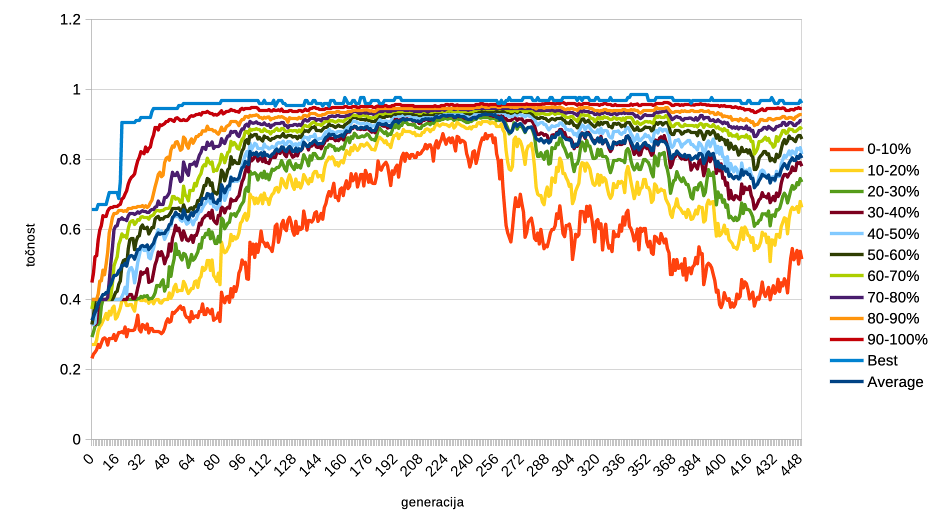
\includegraphics[width=13cm]{wine/3/acc}
    \end{center}
    \caption{Graf točnosti populacije najboljšega agenta tretjega nabora skozi generacije.}
    \label{fig:wine_acc_3}
\end{figure}

\begin{figure}[H]
    \begin{center}
        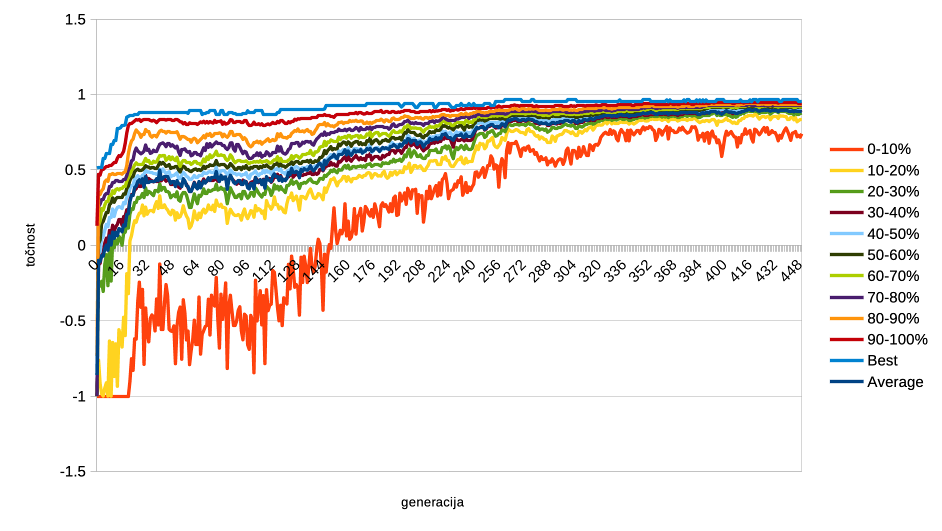
\includegraphics[width=13cm]{wine/3/mcc}
    \end{center}
    \caption{Graf MCC populacije najboljšega agenta tretjega nabora skozi generacije.}
    \label{fig:wine_mcc_3}
\end{figure}

\begin{figure}[H]
    \begin{center}
        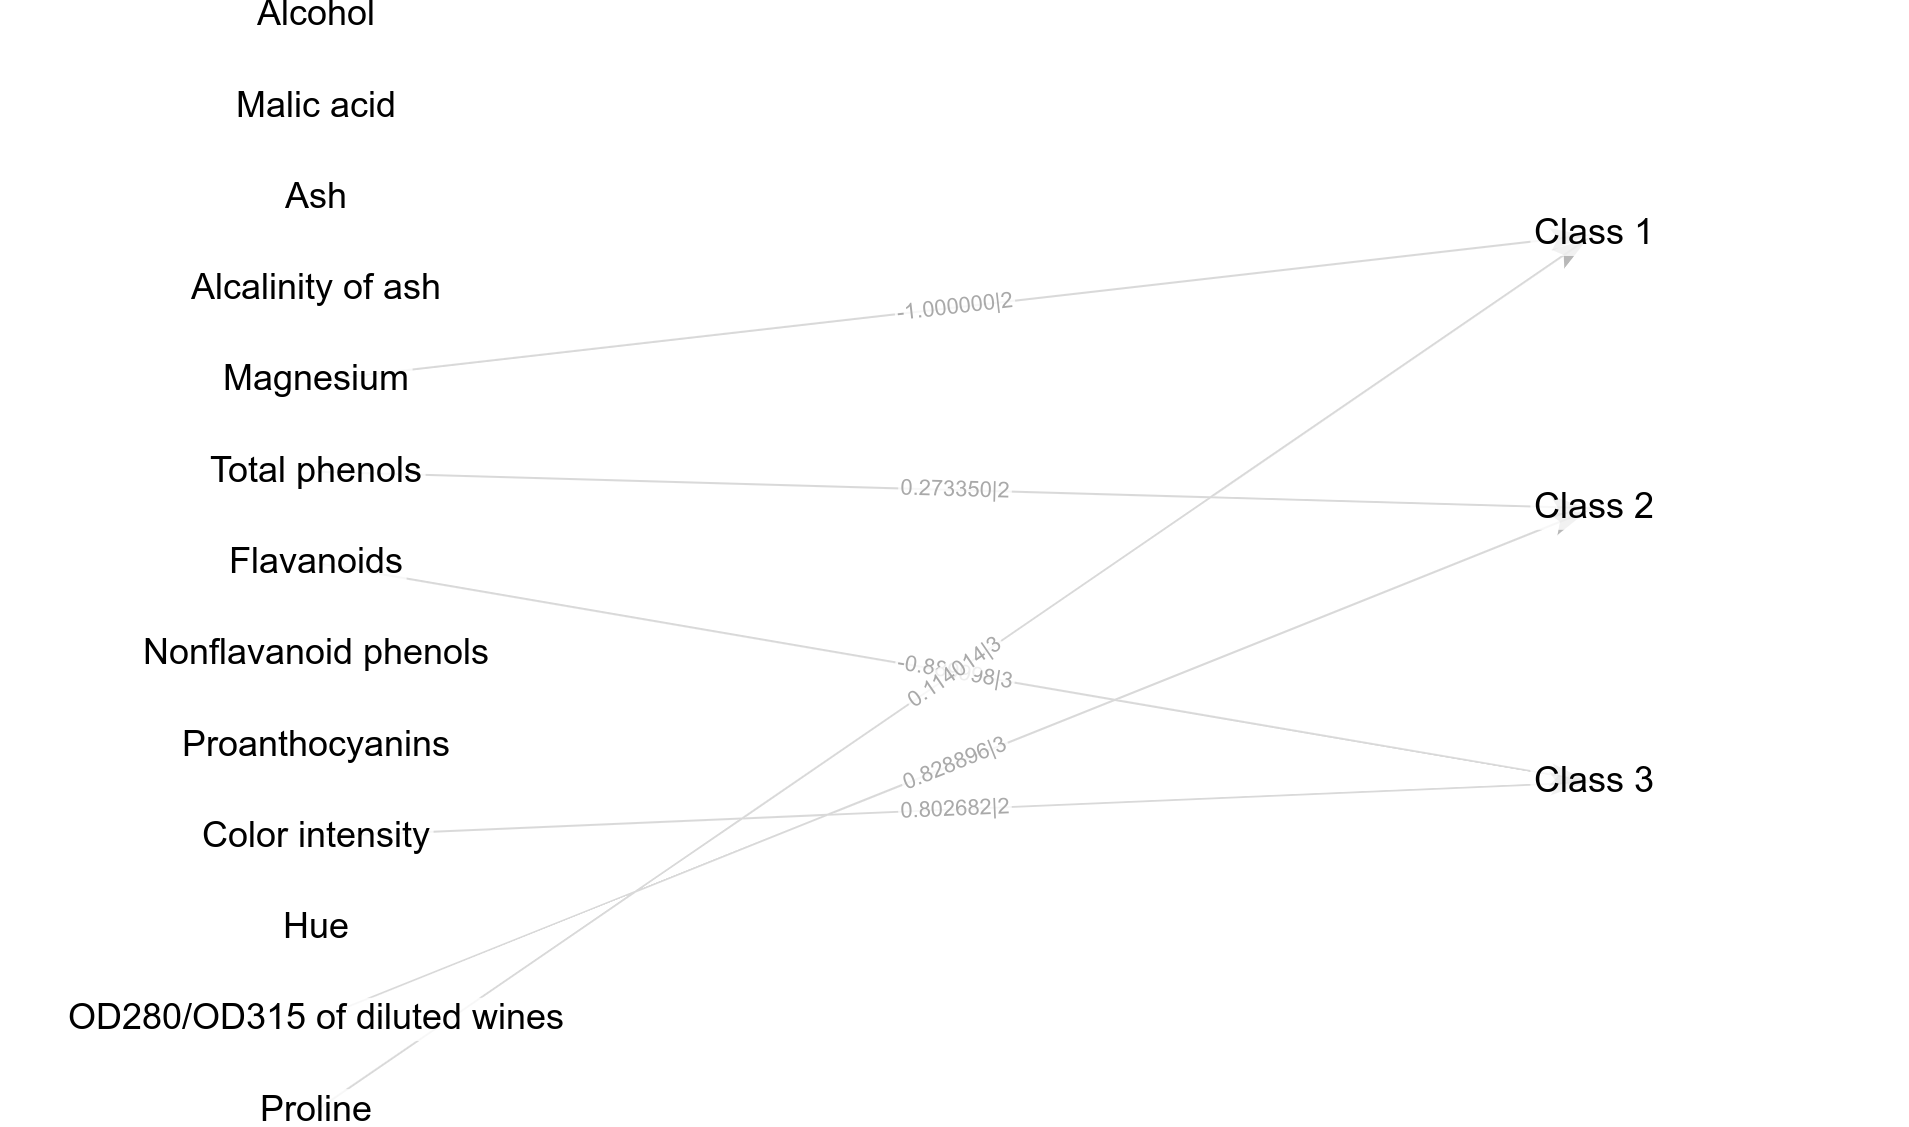
\includegraphics[width=13cm]{wine/3/acc_g}
    \end{center}
    \caption{Vizualizacija najbolj točnega agenta tretjega nabora. Vsebuje 11 povezav.}
    \label{fig:wine_acc_3_g}
\end{figure}

\begin{figure}[H]
    \begin{center}
        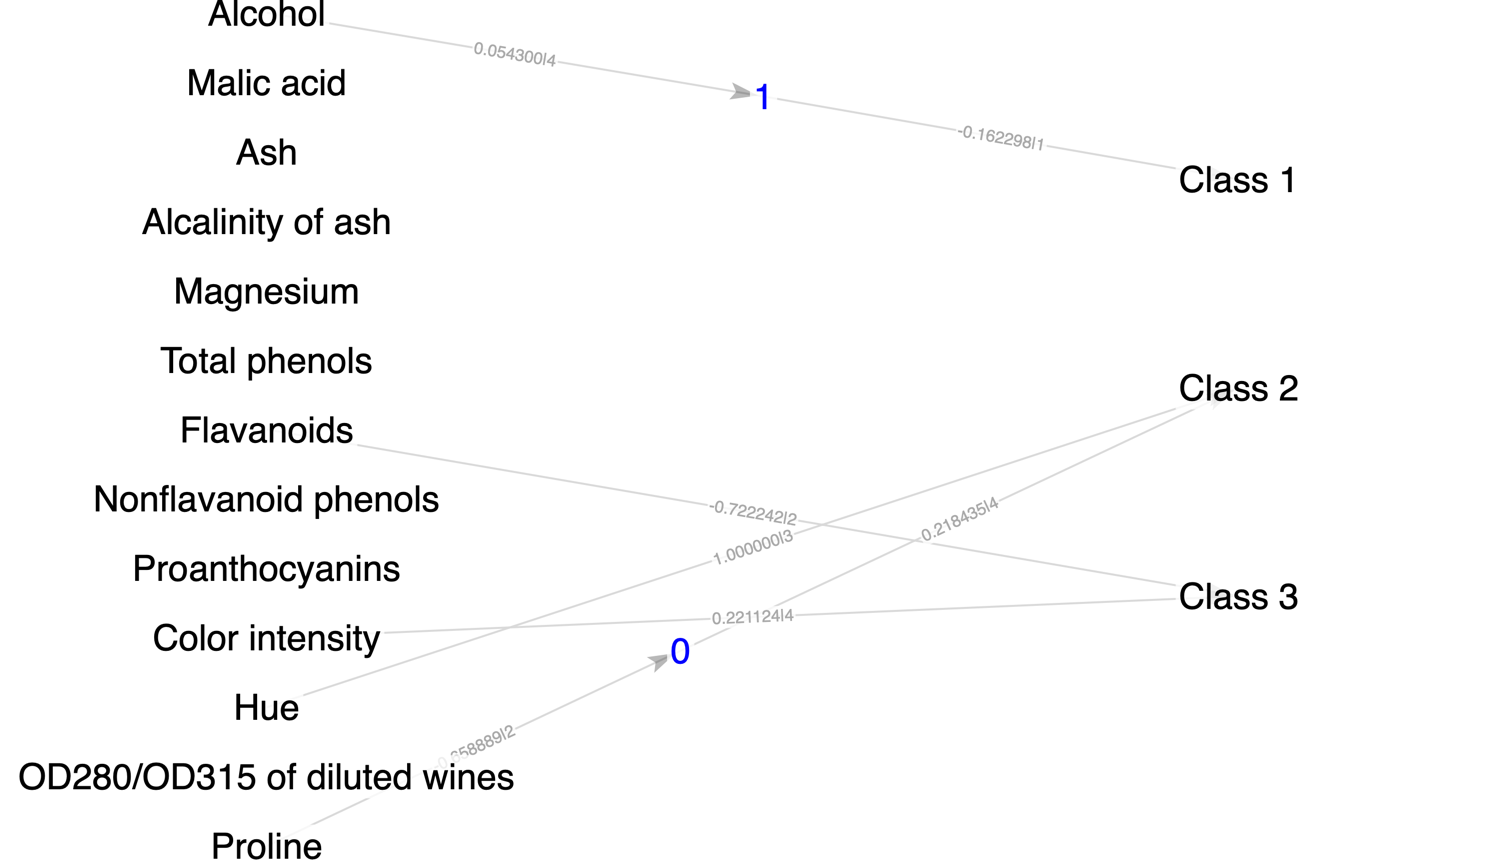
\includegraphics[width=13cm]{wine/3/mcc_g}
    \end{center}
    \caption{Vizualizacija agenta z največjim MCC tretjega nabora. Vsebuje 2 globoki vozlišči in 7 povezav.}
    \label{fig:wine_mcc_3_g}
\end{figure}

\section{Car Evaluation}\label{sec:dodatek-car-test}
%% arrowLength=10
%% linkWidth=3
%% input fy=50*node.pos
%% output fx=350
%% output fy=50*node.pos+50
%% MAX_FONT_SIZE=8
\begin{table}[H]
    \begin{center}
        \begin{tabular}{||l c c c||}
            \hline
            & 1        & 2        & 3 \\ [0.5ex]
            \hline
            velikost populacije              & 200      & 250      & 350      \\
            \hline
            največje število vmesnih vozlišč & 15       & 20       & 40       \\
            \hline
            največje število povezav         & 30       & 50       & 100      \\
            \hline
            največje število prečkanj        & 2        & 3        & 4        \\
            \hline
            delež mutiranih potomcev         & 10\%     & 10\%     & 10\%     \\
            \hline
            prispevek kompleksnosti          & -0.00001 & -0.00001 & -0.00001 \\
            \hline
            število generacij                & 200      & 200      & 300      \\
            \hline
        \end{tabular}
    \end{center}
    \caption{Nabori inicializacijskih parametrov poganjanja na množici Car Evaluation.}
    \label{tab:param_car}
\end{table}

\subsection{Prvi nabor}\label{subsec:dodatek-car-prvi-nabor}
%%"/home/jure/CLionProjects/Neuroevolution/datasets/car/car.data" 200 15 30 2 true 0.1 100 true -0.00001 200 ACC
\begin{table}[H]
    \begin{center}
        \begin{tabular}{|| c | c c || c c ||}
            \hline
            \multirow{2}{*}{št. zagona} & \multicolumn{2}{c||}{točnost najboljšega agenta} & \multicolumn{2}{c||}{MKK najboljšega agenta} \\ \cline{2-5}
            & učna   & testna          & učna  & testna                  \\
            \hline
            1         & 71.7\% & 71.4\%          & 0.507 & 0.454                   \\
            \hline
            2         & 72.6\% & 73.4\%          & 0.477 & 0.486                   \\
            \hline
            3         & 74.0\% & \textbf{73.6\%} & 0.457 & 0.431                   \\
            \hline
            4         & 71.4\% & 71.0\%          & 0.496 & \textbf{0.487 (73.7\%)} \\
            \hline
            5         & 72.1\% & 70.7\%          & 0.483 & 0.403                   \\
            \hline
            povprečje & 72.4\% & 72.0\%          & 0.478 & 0.452                   \\
            \hline
            $\sigma$  & 0.009  & 0.012           & 0.017 & 0.032                   \\
            \hline
        \end{tabular}
    \end{center}
    \caption{Rezultat prvega nabora parametrov.}
    \label{tab:car_result_1}
\end{table}

\begin{table}[H]
    \centering
    \begin{tabular}{||rccccc||}
        \hline
        razred       & unacceptable & acceptable & good & very good & vsota \\ \hline
        unacceptable & 354          & 0          & 9    & 0         & 363   \\ \hline
        acceptable   & 100          & 14         & 1    & 0         & 115   \\ \hline
        good         & 8            & 0          & 13   & 0         & 21    \\ \hline
        very good    & 10           & 1          & 8    & 0         & 19    \\ \hline
        vsota        & 472          & 15         & 31   & 0         & 518   \\ \hline
    \end{tabular}
    \caption{Matrika zmot najbolj točnega agenta prvega nabora. Agent ne more napovedati razreda \enquote{zelo dobro}.}
    \label{tab:car_acc_1}
\end{table}

\begin{table}[H]
    \centering
    \begin{tabular}{||rccccc||}
        \hline
        razred       & unacceptable & acceptable & good & very good & vsota \\ \hline
        unacceptable & 289          & 74         & 0    & 0         & 363   \\ \hline
        acceptable   & 22           & 93         & 0    & 0         & 115   \\ \hline
        good         & 0            & 21         & 0    & 0         & 21    \\ \hline
        very good    & 0            & 19         & 0    & 0         & 19    \\ \hline
        vsota        & 311          & 207        & 0    & 0         & 518   \\ \hline
    \end{tabular}
    \caption{Matrika zmot agenta z največjim MKK prvega nabora. Agent lahko napove samo razreda \enquote{nesprejemljivo} in \enquote{sprejemljivo}.}
    \label{tab:car_mcc_1}
\end{table}

\begin{figure}[H]
    \begin{center}
        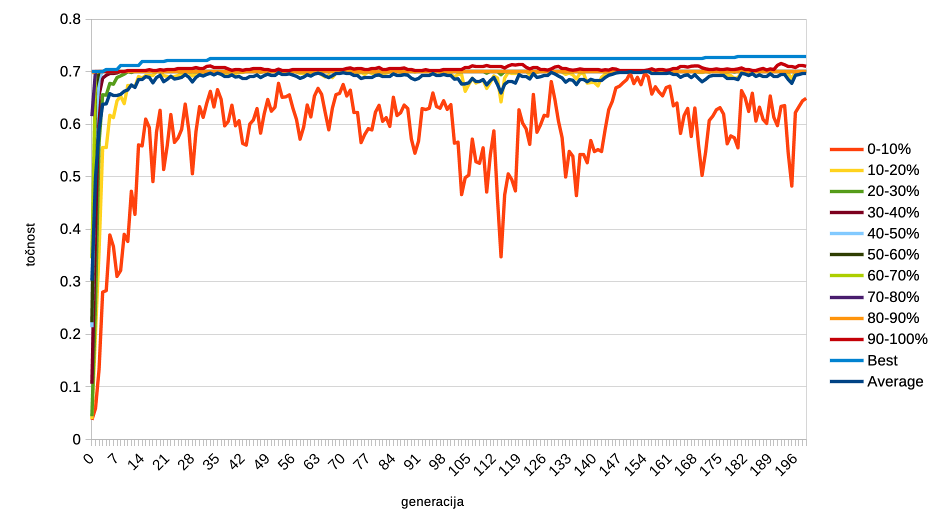
\includegraphics[width=13cm]{car/1/acc}
    \end{center}
    \caption{Graf točnosti populacije najboljšega agenta prvega nabora skozi generacije.}
    \label{fig:car_acc_1}
\end{figure}

\begin{figure}[H]
    \begin{center}
        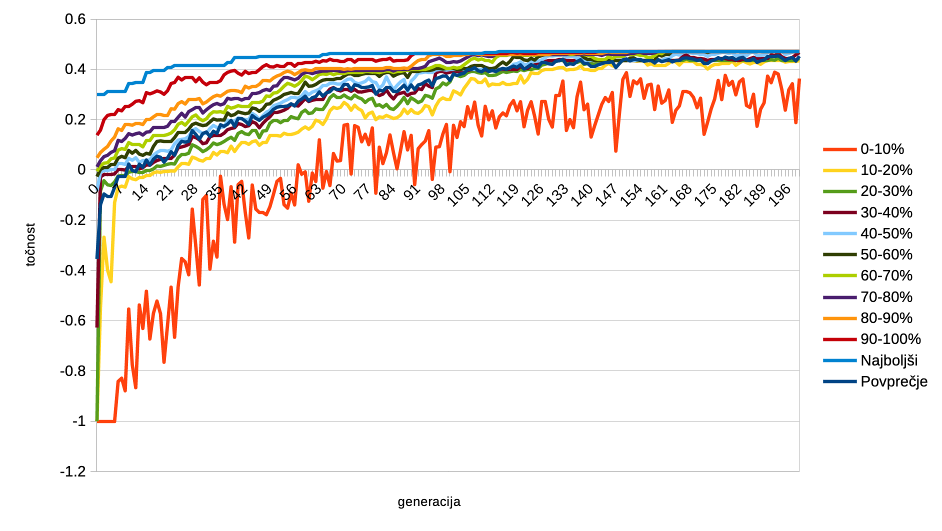
\includegraphics[width=13cm]{car/1/mcc}
    \end{center}
    \caption{Graf MKK populacije najboljšega agenta prvega nabora skozi generacije.}
    \label{fig:car_mcc_1}
\end{figure}

\begin{figure}[H]
    \begin{center}
        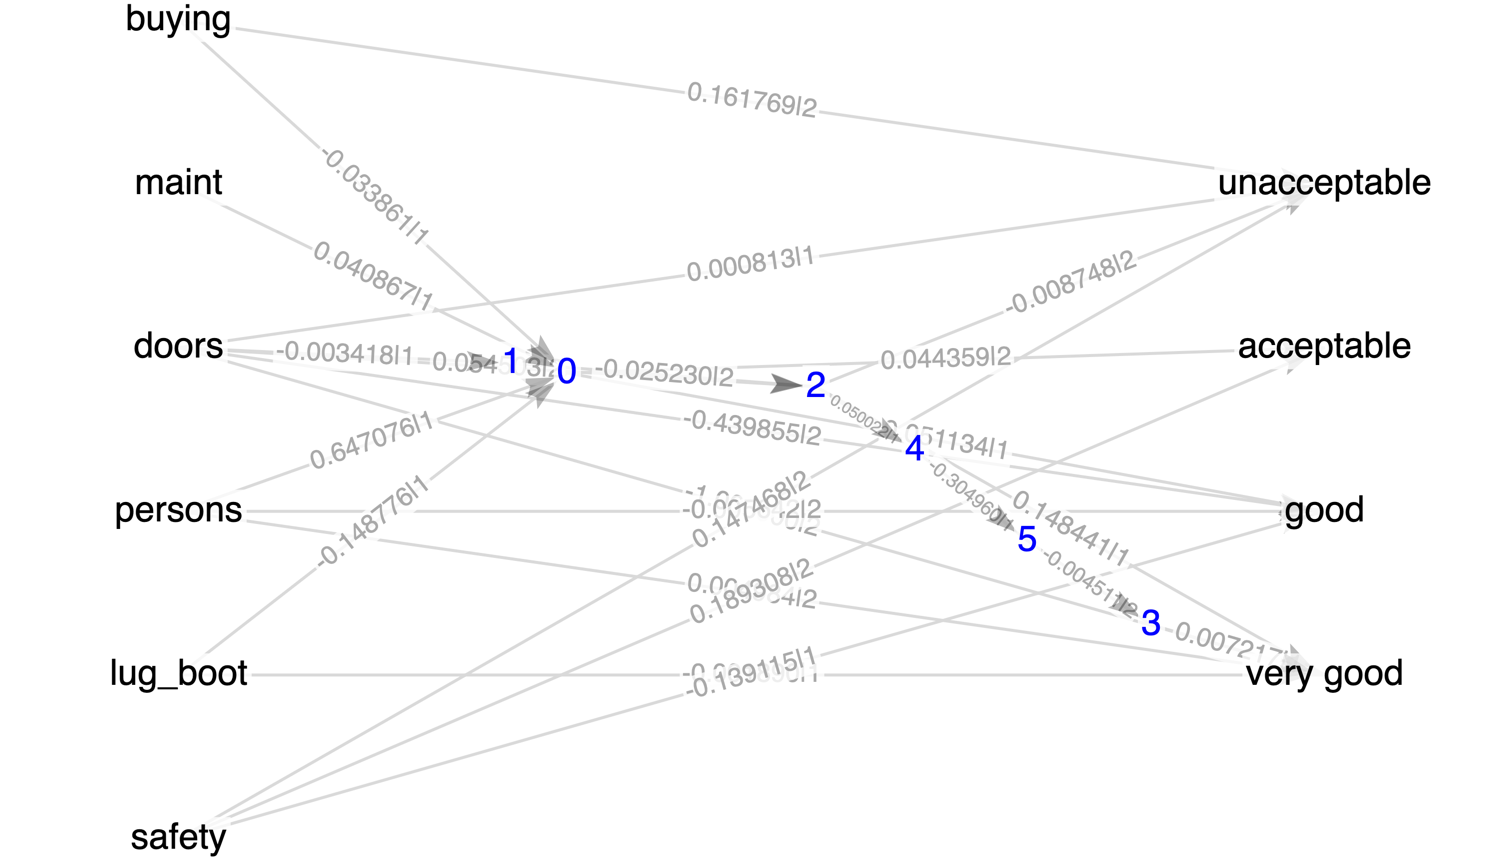
\includegraphics[width=13cm]{car/1/acc_g}
    \end{center}
    \caption{Vizualizacija najbolj točnega agenta prvega nabora. Vsebuje 10 povezav.}
    \label{fig:car_acc_1_g}
\end{figure}

\begin{figure}[H]
    \begin{center}
        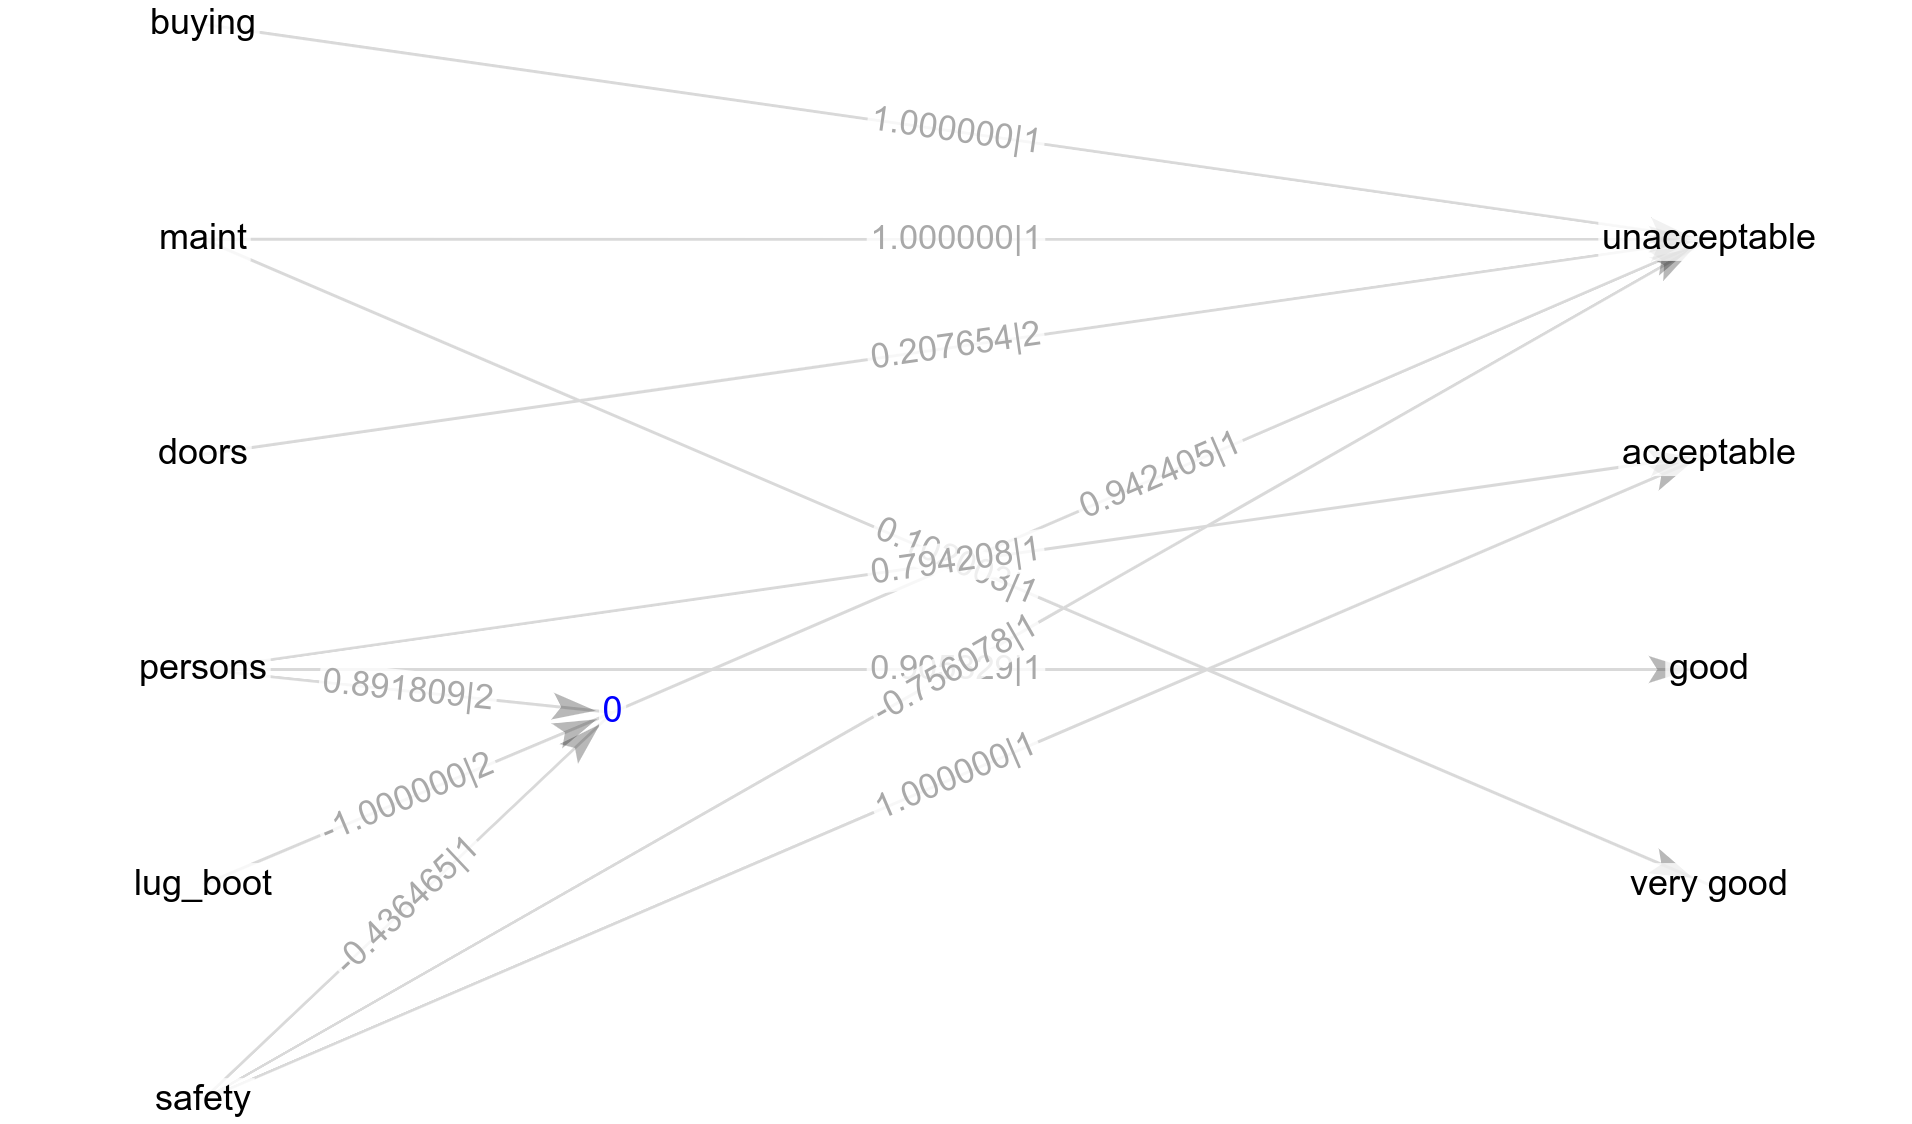
\includegraphics[width=13cm]{car/1/mcc_g}
    \end{center}
    \caption{Vizualizacija agenta z največjim MKK prvega nabora. Vsebuje 1 vmesno vozlišče in 12 povezav.}
    \label{fig:car_mcc_1_g}
\end{figure}

\subsection{Drugi nabor}\label{subsec:dodatek-car-drugi-nabor}
%% 250 20 50 3 true 0.1 125 true -0.00001 200 ACC
\begin{table}[H]
    \begin{center}
        \begin{tabular}{|| c | c c || c c ||}
            \hline
            \multirow{2}{*}{št. zagona} & \multicolumn{2}{c||}{točnost najboljšega agenta} & \multicolumn{2}{c||}{MKK najboljšega agenta} \\ \cline{2-5}
            & učna   & testna          & učna  & testna                  \\
            \hline
            1         & 76.6\% & \textbf{74.3\%} & 0.502 & 0.470                   \\
            \hline
            2         & 74.9\% & 68.3\%          & 0.481 & 0.484                   \\
            \hline
            3         & 71.9\% & 72.0\%          & 0.485 & 0.493                   \\
            \hline
            4         & 72.3\% & 72.8\%          & 0.565 & \textbf{0.585 (75.9\%)} \\
            \hline
            5         & 72.3\% & 71.0\%          & 0.492 & 0.457                   \\
            \hline
            povprečje & 73.6\% & 71.7\%          & 0.505 & 0.498                   \\
            \hline
            $\sigma$  & 0.018  & 0.020            & 0.031 & 0.045                   \\
            \hline
        \end{tabular}
    \end{center}
    \caption{Rezultat drugega nabora parametrov.}
    \label{tab:car_result_2}
\end{table}

\begin{table}[H]
    \centering
    \begin{tabular}{||rccccc||}
        \hline
        razred       & unacceptable & acceptable & good & very good & vsota \\ \hline
        unacceptable & 325          & 38         & 0    & 0         & 363   \\ \hline
        acceptable   & 55           & 60         & 0    & 0         & 115   \\ \hline
        good         & 0            & 21         & 0    & 0         & 21    \\ \hline
        very good    & 0            & 19         & 0    & 0         & 19    \\ \hline
        vsota        & 380          & 138        & 0    & 0         & 518   \\ \hline
    \end{tabular}
    \caption{Matrika zmot najbolj točnega agenta drugega nabora. Agent lahko napove samo razreda \enquote{nesprejemljivo} in \enquote{sprejemljivo}.}
    \label{tab:car_acc_2}
\end{table}

\begin{table}[H]
    \centering
    \begin{tabular}{||rccccc||}
        \hline
        razred       & unacceptable & acceptable & good & very good & vsota \\ \hline
        unacceptable & 271          & 67         & 0    & 25        & 363   \\ \hline
        acceptable   & 7            & 107        & 0    & 1         & 115   \\ \hline
        good         & 0            & 9          & 0    & 12        & 21    \\ \hline
        very good    & 0            & 4          & 0    & 15        & 19    \\ \hline
        vsota        & 278          & 187        & 0    & 53        & 518   \\ \hline
    \end{tabular}
    \caption{Matrika zmot agenta z največjim MKK drugega nabora. Agent ne more napovedati razreda \enquote{dobro}.}
    \label{tab:car_mcc_2}
\end{table}

\begin{figure}[H]
    \begin{center}
        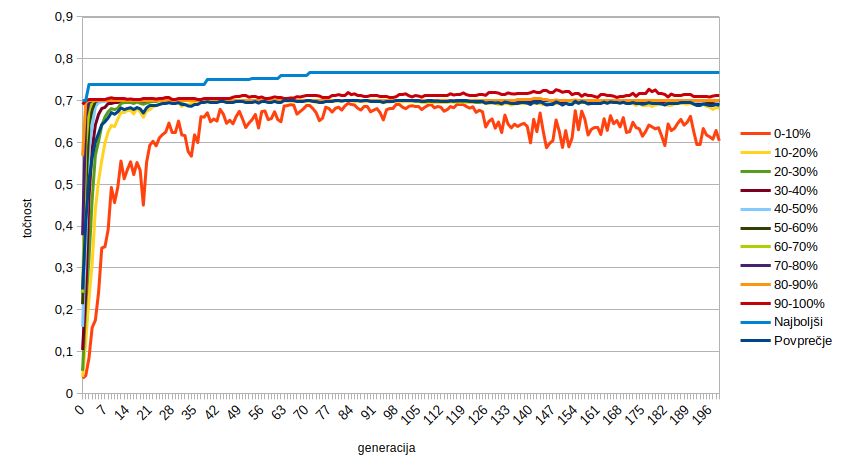
\includegraphics[width=13cm]{car/2/acc}
    \end{center}
    \caption{Graf točnosti populacije najboljšega agenta drugega nabora skozi generacije.}
    \label{fig:car_acc_2}
\end{figure}

\begin{figure}[H]
    \begin{center}
        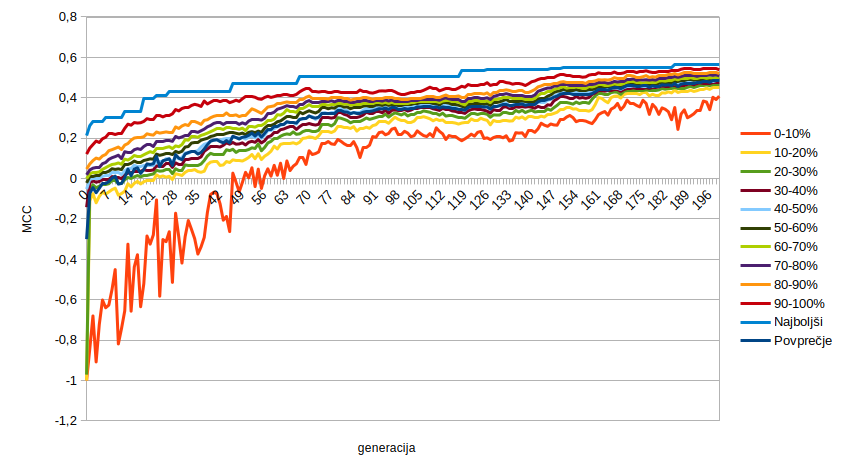
\includegraphics[width=13cm]{car/2/mcc}
    \end{center}
    \caption{Graf MKK populacije najboljšega agenta drugega nabora skozi generacije.}
    \label{fig:car_mcc_2}
\end{figure}

\begin{figure}[H]
    \begin{center}
        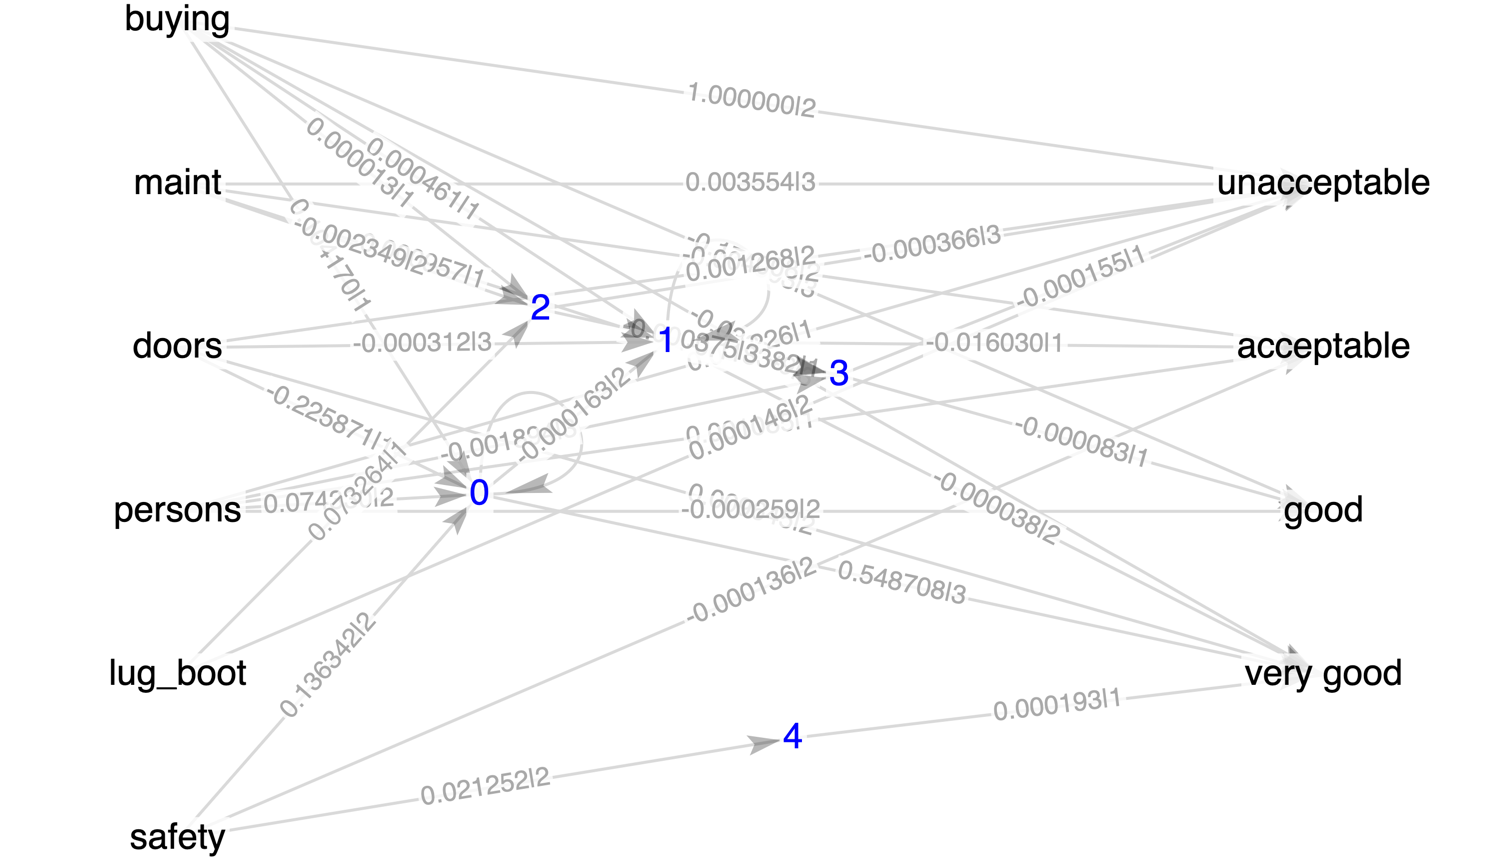
\includegraphics[width=13cm]{car/2/acc_g}
    \end{center}
    \caption{Vizualizacija najbolj točnega agenta drugega nabora. Vsebuje 1 vmesno vozlišče in 16 povezav.}
    \label{fig:car_acc_2_g}
\end{figure}

\begin{figure}[H]
    \begin{center}
        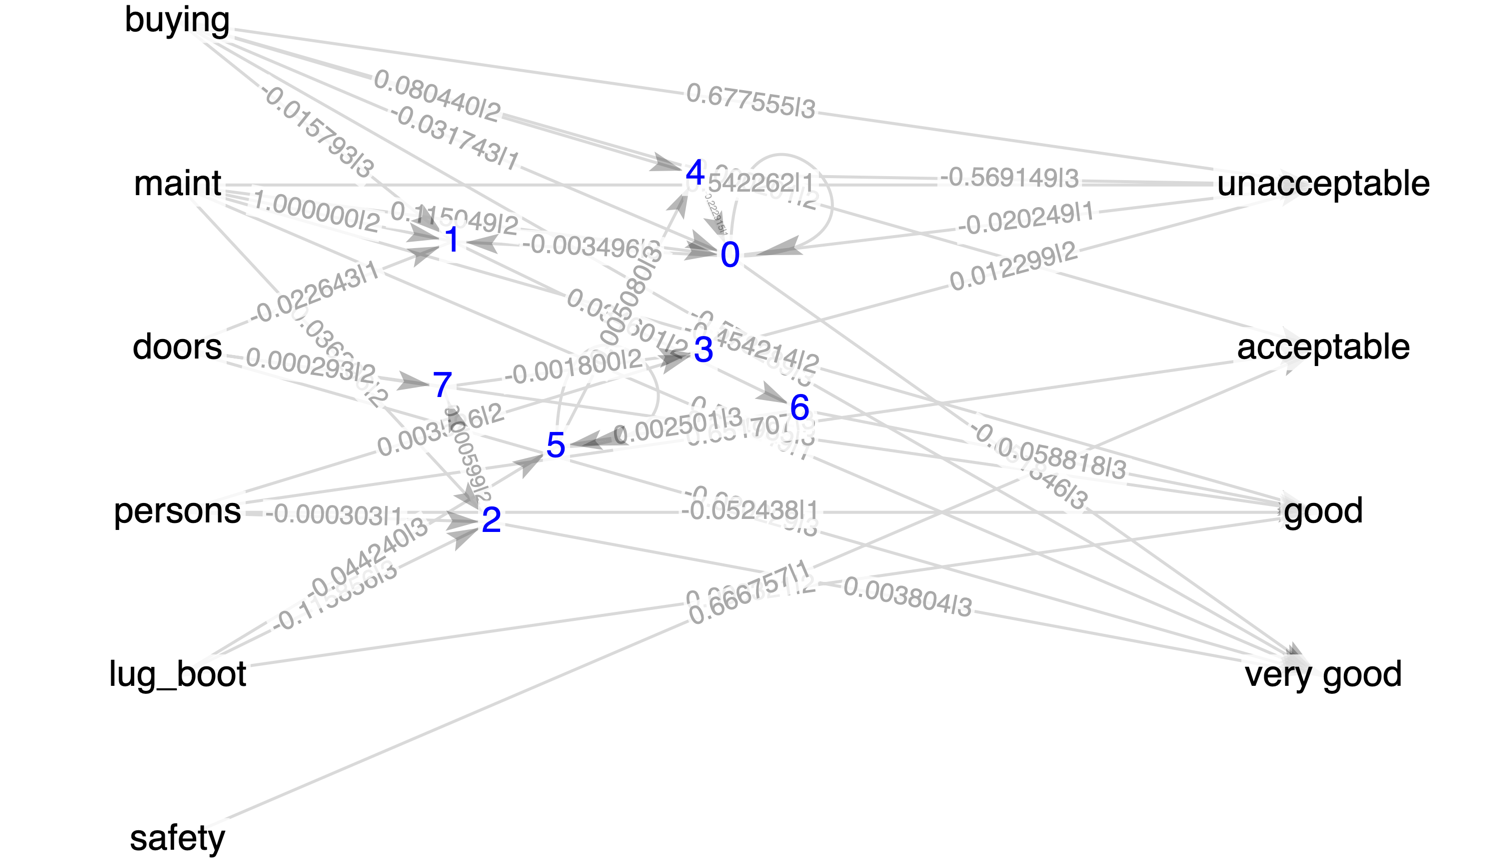
\includegraphics[width=13cm]{car/2/mcc_g}
    \end{center}
    \caption{Vizualizacija agenta z največjim MKK drugega nabora. Vsebuje 13 povezav.}
    \label{fig:car_mcc_2_g}
\end{figure}

\newpage

\subsection{Tretji nabor}\label{subsec:dodatek-car-tretji-nabor}
%% 350 40 100 4 true 0.1 175 true -0.00001 300 ACC
\begin{table}[H]
    \begin{center}
        \begin{tabular}{|| c | c c || c c ||}
            \hline
            \multirow{2}{*}{št. zagona} & \multicolumn{2}{c||}{točnost najboljšega agenta} & \multicolumn{2}{c||}{MKK najboljšega agenta} \\ \cline{2-5}
            & učna   & testna          & učna  & testna                  \\
            \hline
            1         & 73.6\% & \textbf{73.6\%} & 0.510 & 0.498                   \\
            \hline
            2         & 73.1\% & 71.2\%          & 0.486 & 0.502                   \\
            \hline
            3         & 72.4\% & 70.8\%          & 0.493 & 0.462                   \\
            \hline
            4         & 73.5\% & 72.0\%          & 0.468 & 0.467                   \\
            \hline
            5         & 72.7\% & 72.8\%          & 0.516 & \textbf{0.539 (73.7\%)} \\
            \hline
            povprečje & 73.1\% & 72.1\%          & 0.495 & 0.494                   \\
            \hline
            $\sigma$  & 0.005  & 0.010           & 0.017 & 0.028                   \\
            \hline
        \end{tabular}
    \end{center}
    \caption{Rezultat tretjega nabora parametrov.}
    \label{tab:car_result_3}
\end{table}

\begin{table}[H]
    \centering
    \begin{tabular}{||rccccc||}
        \hline
        razred       & unacceptable & acceptable & good & very good & vsota \\ \hline
        unacceptable & 325          & 38         & 0    & 0         & 363   \\ \hline
        acceptable   & 59           & 56         & 0    & 0         & 115   \\ \hline
        good         & 4            & 17         & 0    & 0         & 21    \\ \hline
        very good    & 0            & 19         & 0    & 0         & 19    \\ \hline
        vsota        & 388          & 130        & 0    & 0         & 518   \\ \hline
    \end{tabular}
    \caption{Matrika zmot najbolj točnega agenta tretjega nabora. Agent lahko napove samo razreda \enquote{nesprejemljivo} in \enquote{sprejemljivo}.}
    \label{tab:car_acc_3}
\end{table}

\begin{table}[H]
    \centering
    \begin{tabular}{||rccccc||}
        \hline
        razred       & unacceptable & acceptable & good & very good & vsota \\ \hline
        unacceptable & 270          & 66         & 0    & 27        & 363   \\ \hline
        acceptable   & 10           & 103        & 0    & 2         & 115   \\ \hline
        good         & 0            & 10         & 0    & 11        & 21    \\ \hline
        very good    & 0            & 10         & 0    & 9         & 19    \\ \hline
        vsota        & 280          & 189        & 0    & 49        & 518   \\ \hline
    \end{tabular}
    \caption{Matrika zmot agenta z največjim MKK tretjega nabora. Agent ne more napovedati razreda \enquote{dobro}.}
    \label{tab:car_mcc_3}
\end{table}

\begin{figure}[H]
    \begin{center}
        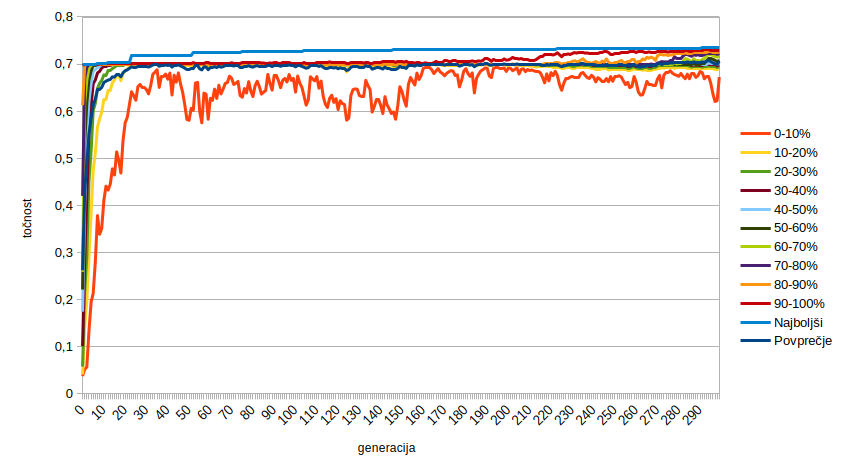
\includegraphics[width=13cm]{car/3/acc}
    \end{center}
    \caption{Graf točnosti populacije najboljšega agenta tretjega nabora skozi generacije.}
    \label{fig:car_acc_3}
\end{figure}

\begin{figure}[H]
    \begin{center}
        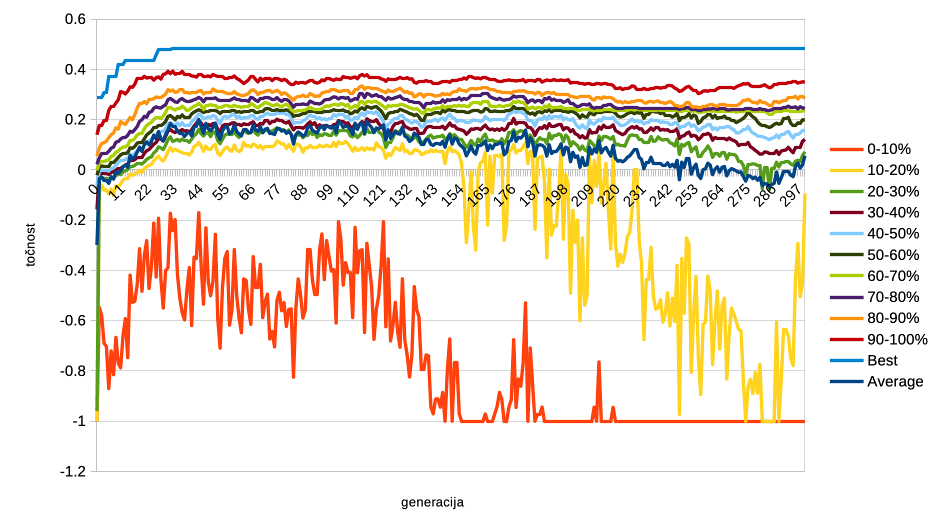
\includegraphics[width=13cm]{car/3/mcc}
    \end{center}
    \caption{Graf MKK populacije najboljšega agenta tretjega nabora skozi generacije.}
    \label{fig:car_mcc_3}
\end{figure}

\begin{figure}[H]
    \begin{center}
        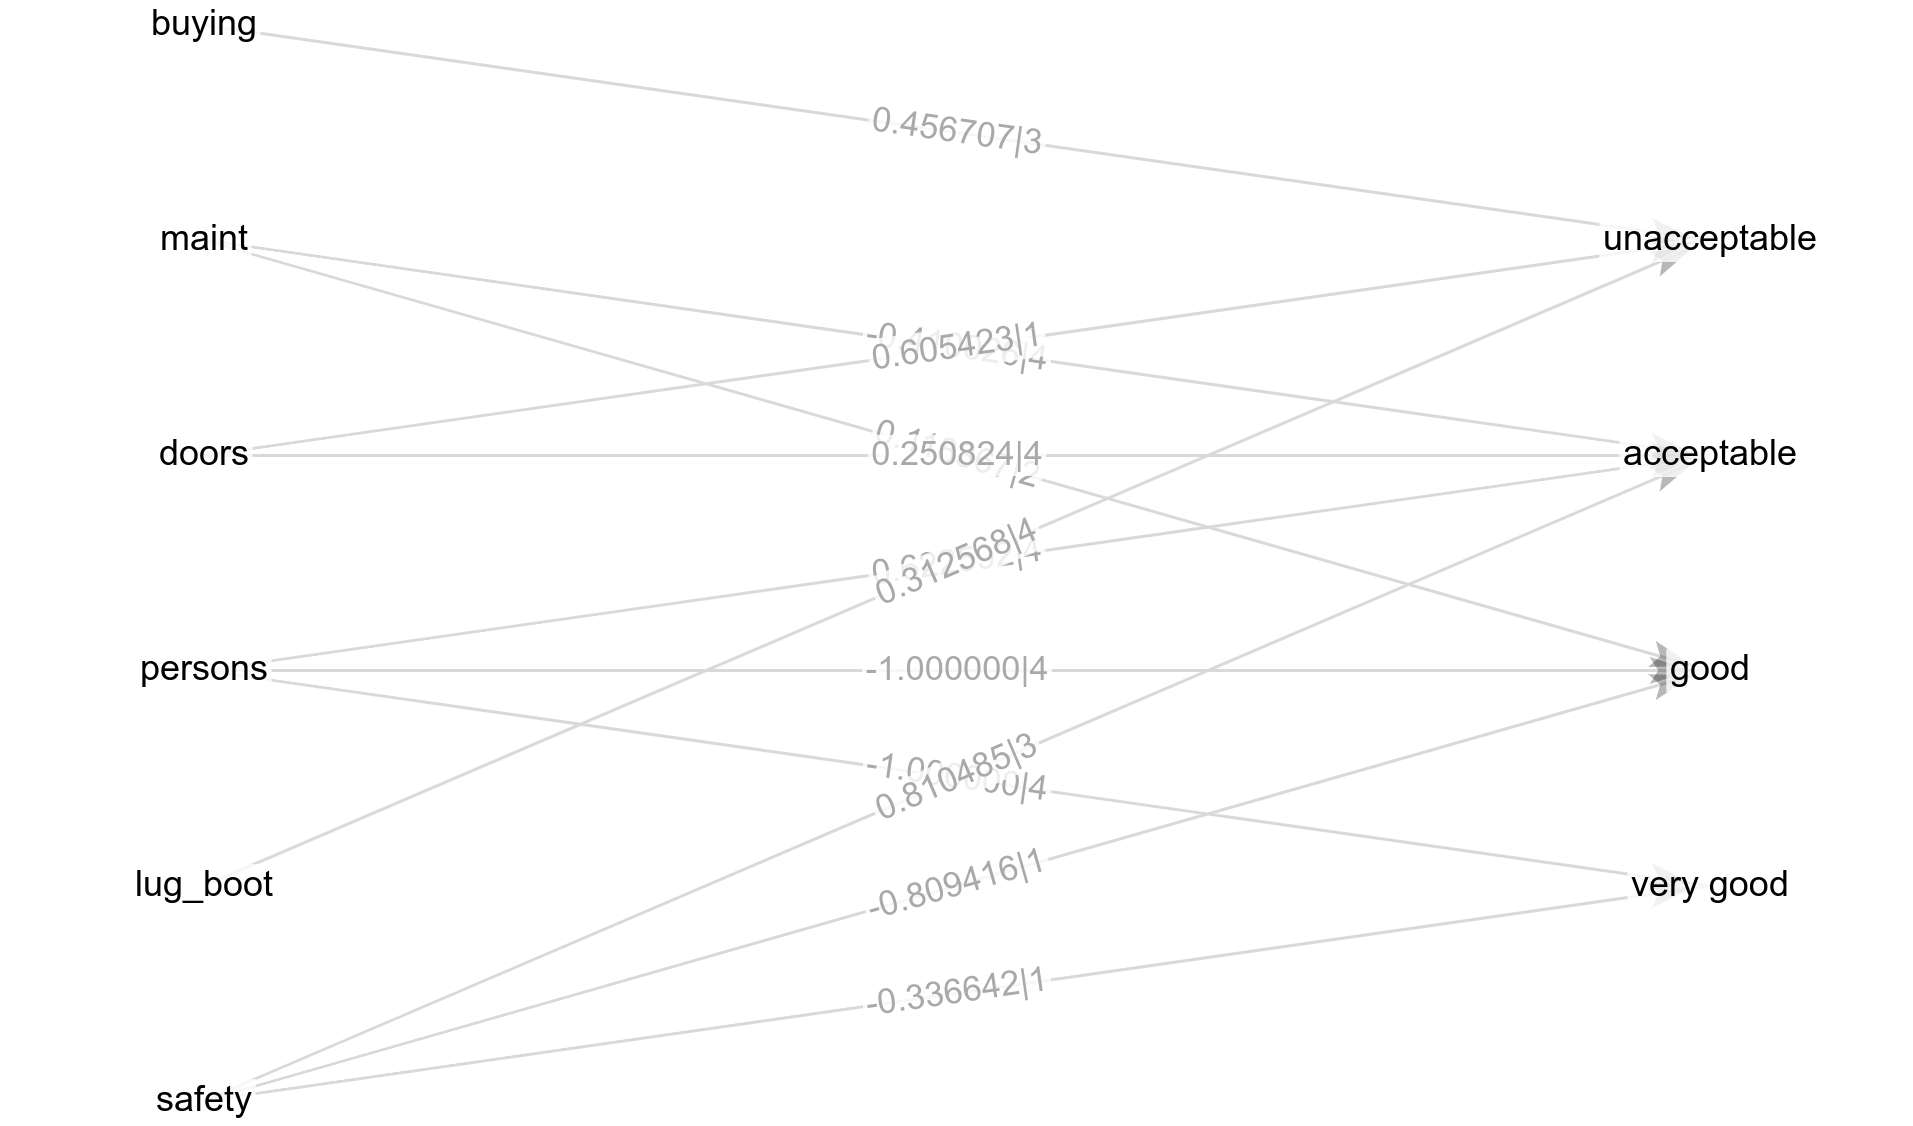
\includegraphics[width=13cm]{car/3/acc_g}
    \end{center}
    \caption{Vizualizacija najbolj točnega agenta tretjega nabora. Vsebuje 12 povezav.}
    \label{fig:car_acc_3_g}
\end{figure}

\begin{figure}[H]
    \begin{center}
        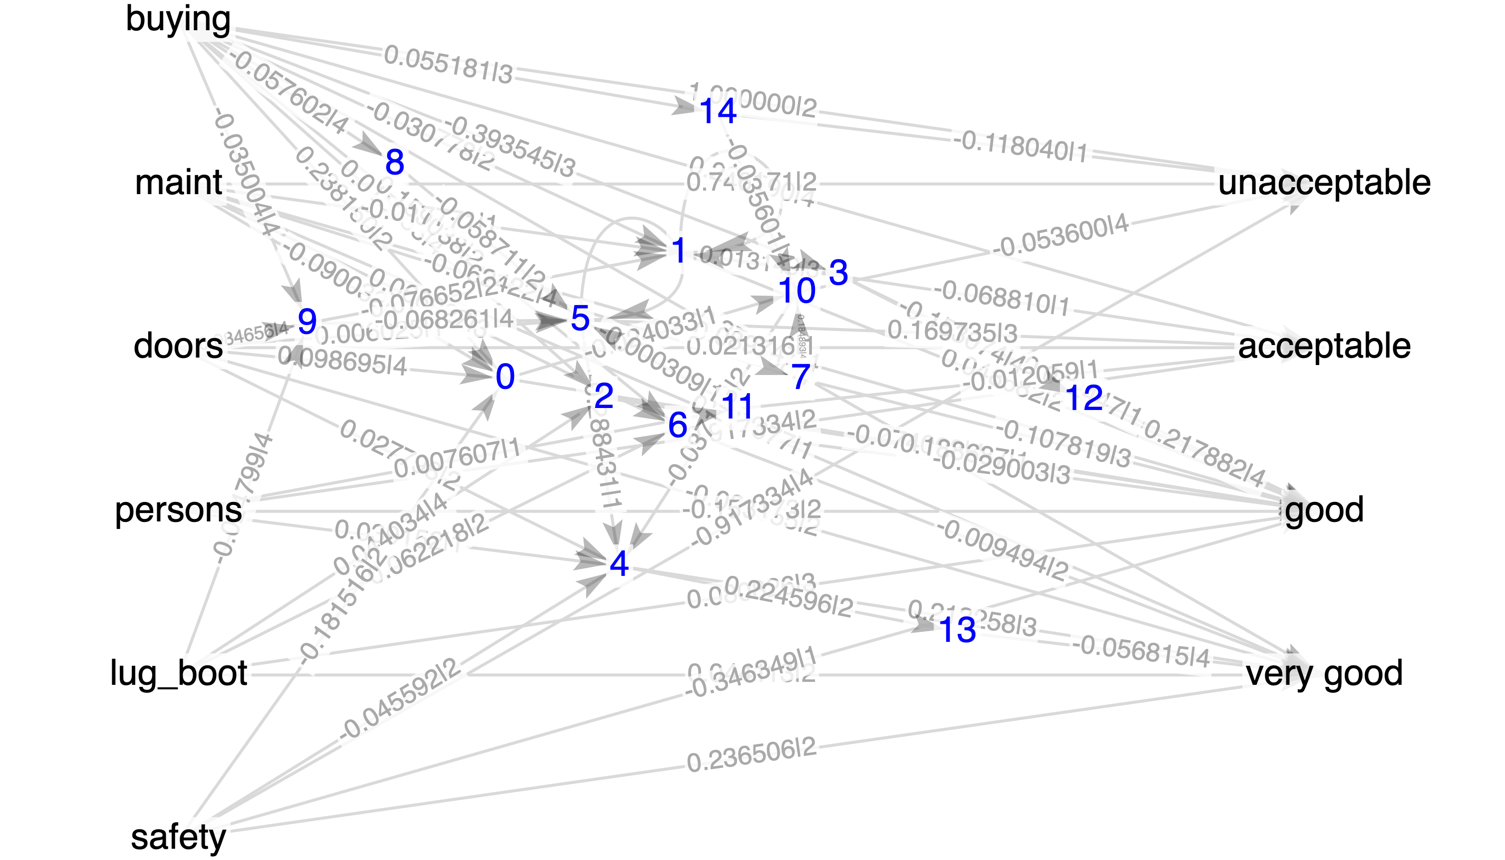
\includegraphics[width=13cm]{car/3/mcc_g}
    \end{center}
    \caption{Vizualizacija agenta z največjim MKK drugega nabora. Vsebuje 13 povezav.}
    \label{fig:car_mcc_3_g}
\end{figure}

\section{Shuttle}\label{sec:dodatek-statlog-test}
%% arrowLength=10
%% linkWidth=3
%% input fy=50*node.pos
%% output fx=550
%% output fy=50*node.pos+25
%% MAX_FONT_SIZE=8
Imena razredov v glavah matrik zmot so okrajšana zaradi formatiranja dokumenta.
\begin{table}[H]
    \begin{center}
        \begin{tabular}{||l c c c||}
            \hline
            & 1        & 2        & 3 \\ [0.5ex]
            \hline
            velikost populacije               & 200      & 250      & 350      \\
            \hline
            največje število globokih vozlišč & 15       & 20       & 40       \\
            \hline
            največje število povezav          & 30       & 50       & 100      \\
            \hline
            največje število prečkanj         & 2        & 3        & 4        \\
            \hline
            delež mutiranih potomcev          & 10\%     & 10\%     & 10\%     \\
            \hline
            prispevek kompleksnosti           & -0.00001 & -0.00001 & -0.00001 \\
            \hline
            število generacij                 & 200      & 250      & 300      \\
            \hline
        \end{tabular}
    \end{center}
    \caption{Nabori inicializacijskih parametrov poganjanja na množici Shuttle.}
    \label{tab:param_statlog}
\end{table}

\subsection{Prvi nabor}\label{subsec:dodatek-statlog-prvi-nabor}
%% branch shuttle
%% 200 15 30 2 true 0.1 100 true -0.00001 200 ACC
\begin{table}[H]
    \begin{center}
        \begin{tabular}{|| c | c c || c c ||}
            \hline
            \multirow{2}{*}{št. zagona} & \multicolumn{2}{c||}{točnost najboljšega agenta} & \multicolumn{2}{c||}{MCC najboljšega agenta} \\ \cline{2-5}
            & učna   & testna          & učna  & testna                  \\
            \hline
            1        & 91.3\% & 91.8\%          & 0.656 & 0.658                   \\
            \hline
            2        & 86.2\% & 86.8\%          & 0.628 & 0.632                   \\
            \hline
            3        & 84.0\% & 84.7\%          & 0.753 & \textbf{0.760 (92.1\%)} \\
            \hline
            4        & 86.8\% & 87.4\%          & 0.572 & 0.578                   \\
            \hline
            5        & 91.8\% & \textbf{92.4\%} & 0.744 & 0.752                   \\
            \hline
            $\sigma$ & 0.030  & 0.030           & 0.069 & 0.070                   \\
            \hline
        \end{tabular}
    \end{center}
    \caption{Rezultat prvega nabora parametrov.}
    \label{tab:statlog_result_1}
\end{table}

\begin{table}[H]
    \centering
    \begin{tabular}{||rcccccccc||}
        \hline
        razred    & RF    & FC & FO & High & Bypass & BC & BO & vsota \\ \hline
        Rad Flow  & 11405 & 0  & 10 & 61   & 1      & 1  & 0  & 11478 \\ \hline
        Fpv Close & 8     & 0  & 0  & 5    & 0      & 0  & 0  & 13    \\ \hline
        Fpv Open  & 11    & 0  & 21 & 6    & 1      & 0  & 0  & 39    \\ \hline
        High      & 998   & 0  & 0  & 1157 & 0      & 0  & 0  & 2155  \\ \hline
        Bypass    & 0     & 0  & 0  & 0    & 808    & 1  & 0  & 809   \\ \hline
        Bpv Close & 1     & 0  & 0  & 1    & 2      & 0  & 0  & 4     \\ \hline
        Bpv Open  & 0     & 0  & 2  & 0    & 0      & 0  & 0  & 2     \\ \hline
        vsota     & 12423 & 0  & 33 & 1230 & 812    & 2  & 0  & 14500 \\ \hline
    \end{tabular}
    \caption{Matrika zmot najbolj točnega agenta prvega nabora. Agent lahko pravilno napove vse razrede razen \enquote{Fpv Close}, \enquote{Bpv Close} in \enquote{Bpv Open}.}
    \label{tab:statlog_acc_1}
\end{table}

\begin{table}[H]
    \centering
    \begin{tabular}{||rcccccccc||}
        \hline
        razred    & RF    & FC & FO & High & Bypass & BC & BO & vsota \\ \hline
        Rad Flow  & 11411 & 0  & 5  & 62   & 0      & 0  & 0  & 11478 \\ \hline
        Fpv Close & 3     & 0  & 0  & 10   & 0      & 0  & 0  & 13    \\ \hline
        Fpv Open  & 36    & 1  & 0  & 1    & 1      & 0  & 0  & 39    \\ \hline
        High      & 1024  & 0  & 0  & 1131 & 0      & 0  & 0  & 2155  \\ \hline
        Bypass    & 0     & 0  & 1  & 1    & 807    & 0  & 0  & 809   \\ \hline
        Bpv Close & 0     & 0  & 0  & 4    & 0      & 0  & 0  & 4     \\ \hline
        Bpv Open  & 2     & 0  & 0  & 0    & 0      & 0  & 0  & 2     \\ \hline
        vsota     & 12476 & 1  & 6  & 1209 & 808    & 0  & 0  & 14500 \\ \hline
    \end{tabular}
    \caption{Matrika zmot agenta z največjim MCC prvega nabora. Agent lahko pravilno napove razrede \enquote{Rad Flow}, \enquote{High} in \enquote{Bypass}.}
    \label{tab:statlog_mcc_1}
\end{table}

\begin{figure}[H]
    \begin{center}
        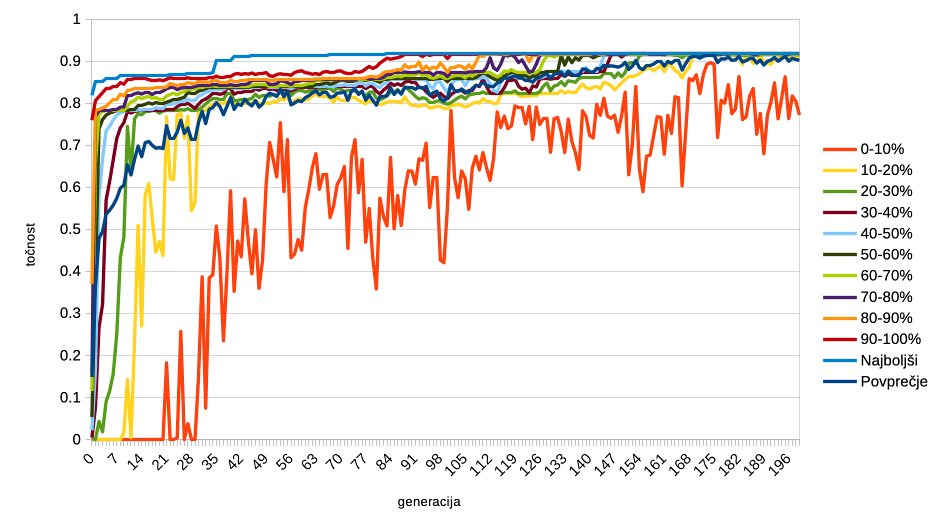
\includegraphics[width=13cm]{shuttle/1/acc}
    \end{center}
    \caption{Graf točnosti populacije najboljšega agenta prvega nabora skozi generacije.}
    \label{fig:statlog_acc_1}
\end{figure}

\begin{figure}[H]
    \begin{center}
        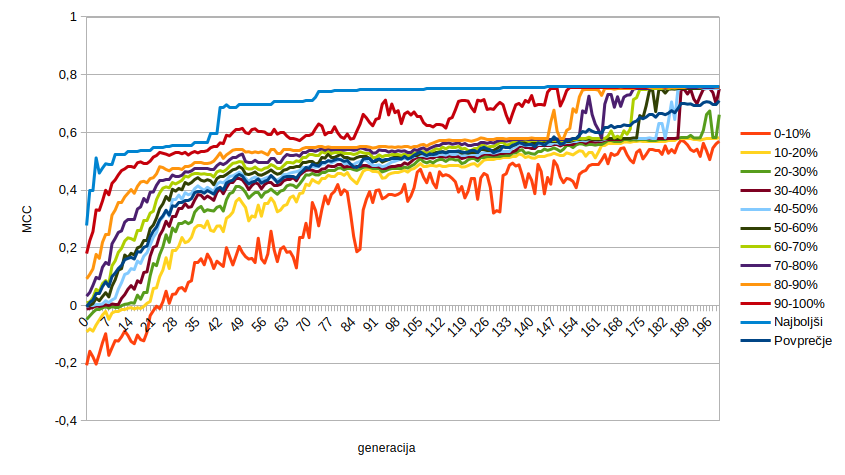
\includegraphics[width=13cm]{shuttle/1/mcc}
    \end{center}
    \caption{Graf MCC populacije najboljšega agenta prvega nabora skozi generacije.}
    \label{fig:statlog_mcc_1}
\end{figure}

\begin{figure}[H]
    \begin{center}
        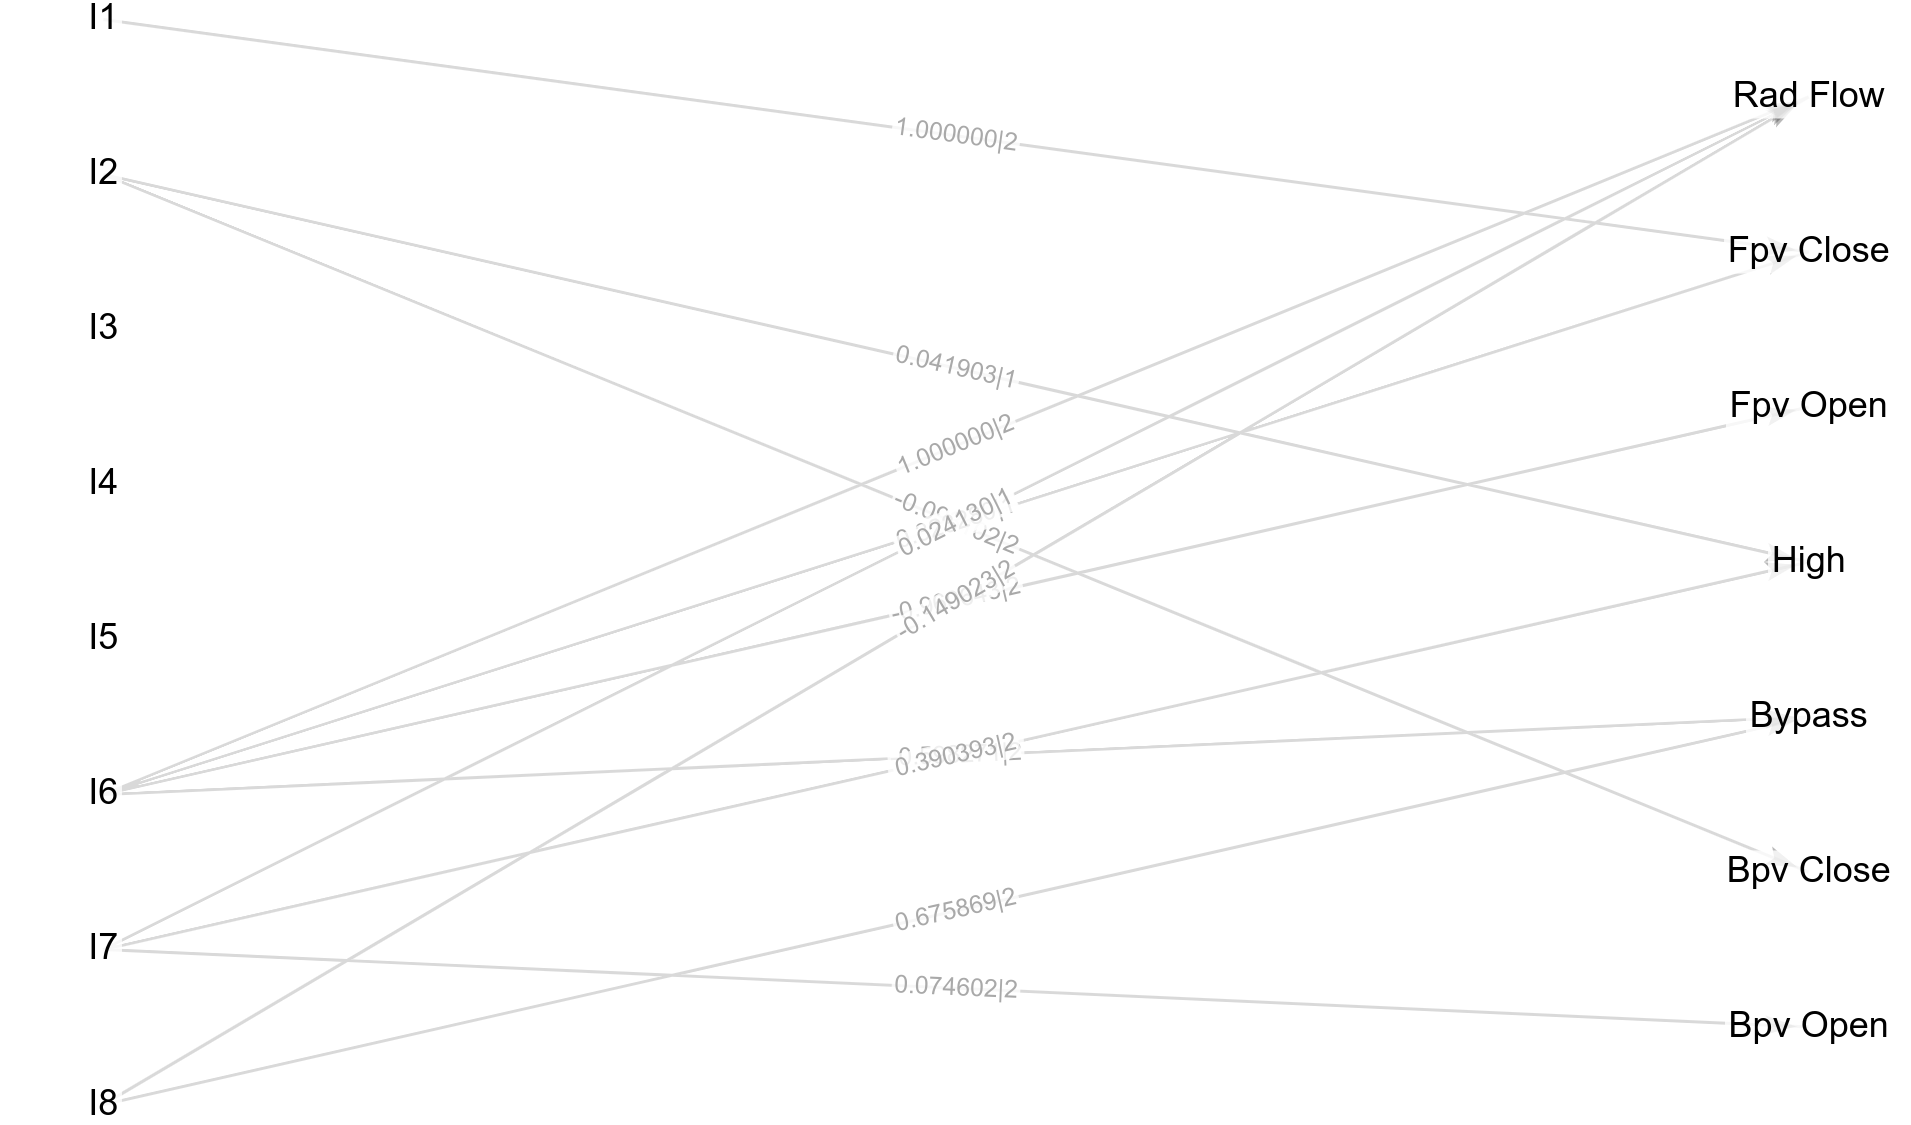
\includegraphics[width=13cm]{shuttle/1/acc_g}
    \end{center}
    \caption{Vizualizacija najbolj točnega agenta prvega nabora. Vsebuje 12 povezav.}
    \label{fig:statlog_acc_1_g}
\end{figure}

\begin{figure}[H]
    \begin{center}
        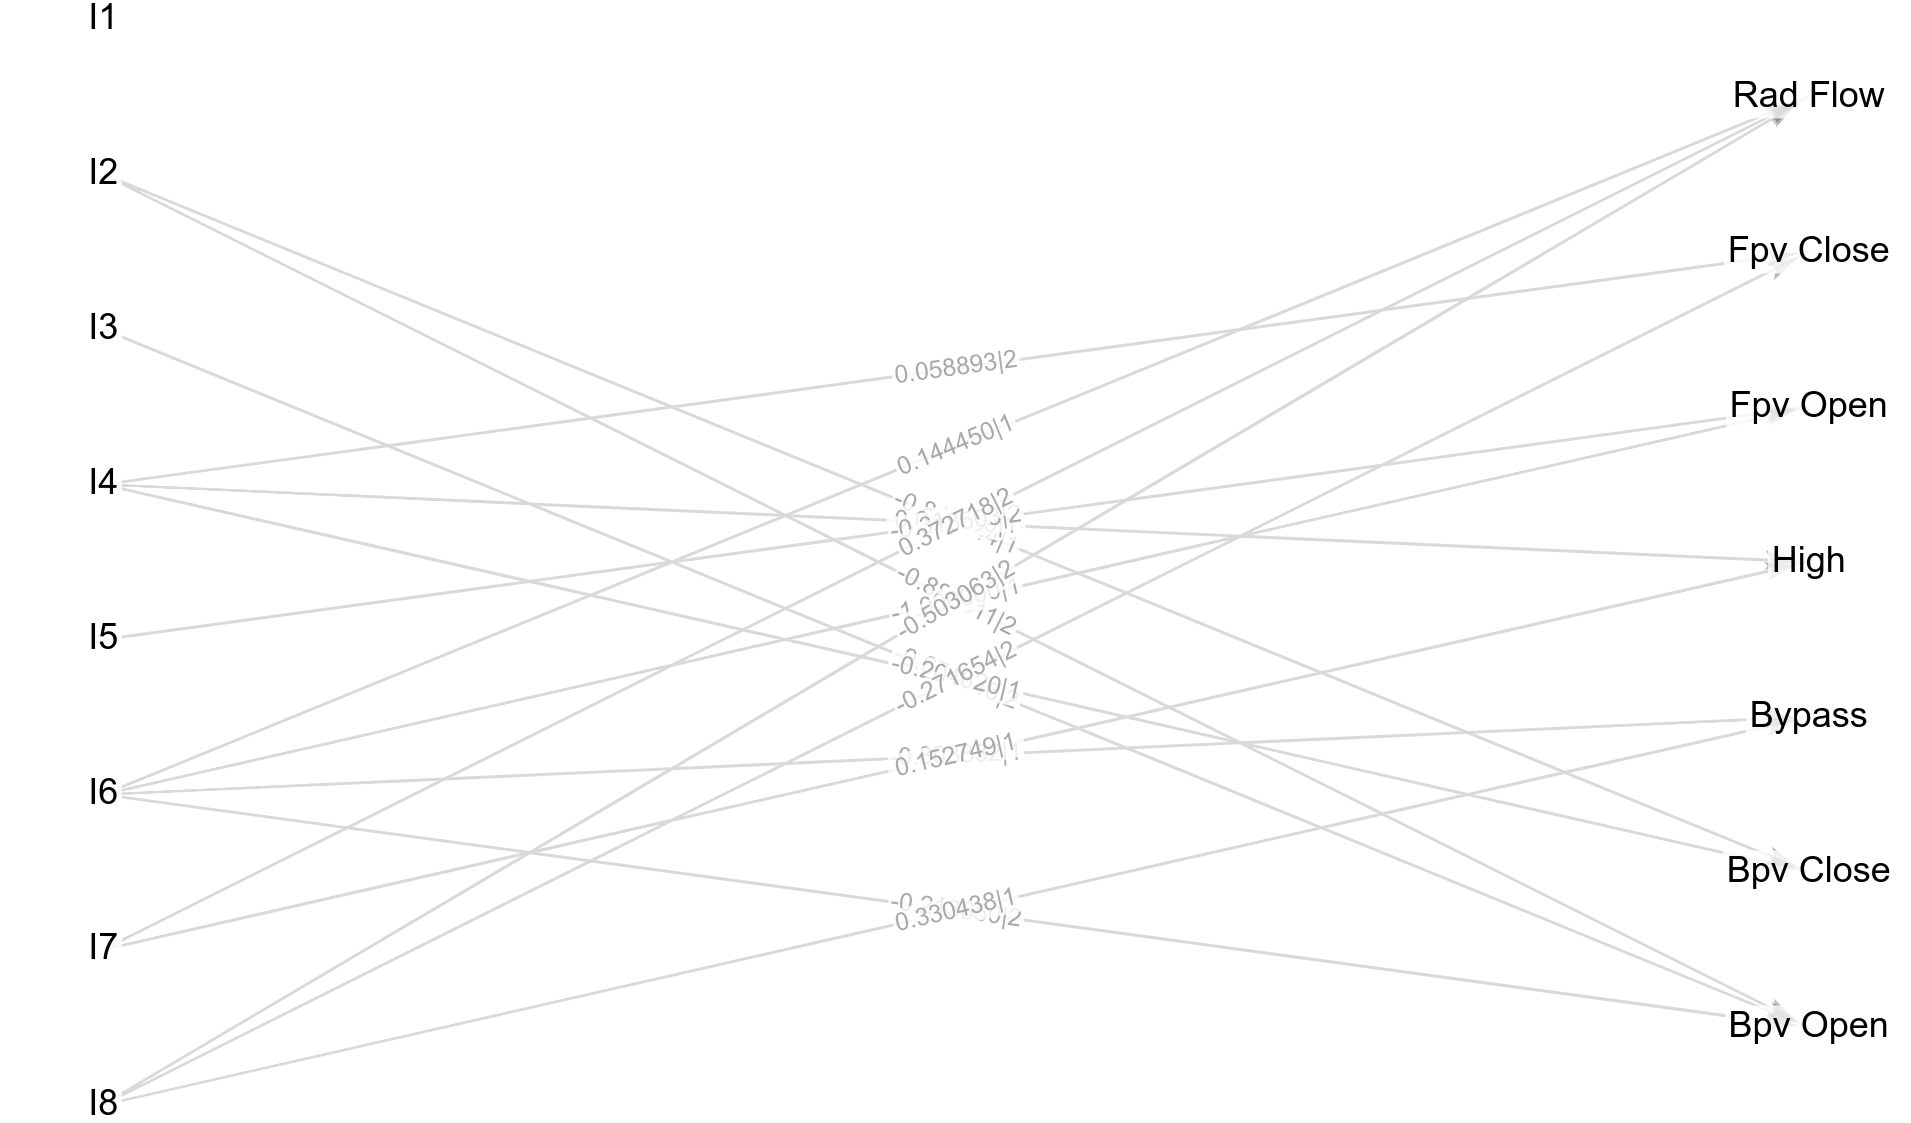
\includegraphics[width=13cm]{shuttle/1/mcc_g}
    \end{center}
    \caption{Vizualizacija agenta z največjim MCC prvega nabora. Vsebuje 1 globoko vozlišče in 21 povezav.}
    \label{fig:statlog_mcc_1_g}
\end{figure}

\subsection{Drugi nabor}\label{subsec:dodatek-statlog-drugi-nabor}
%% 250 20 50 3 true 0.1 125 true -0.00001 250 ACC
\begin{table}[H]
    \begin{center}
        \begin{tabular}{|| c | c c || c c ||}
            \hline
            \multirow{2}{*}{št. zagona} & \multicolumn{2}{c||}{točnost najboljšega agenta} & \multicolumn{2}{c||}{MCC najboljšega agenta} \\ \cline{2-5}
            & učna & testna       & učna & testna           \\
            \hline
            1        & 0\%  & 0\%          & 0    & 0                \\
            \hline
            2        & 0\%  & 0\%          & 0    & 0                \\
            \hline
            3        & 0\%  & 0\%          & 0    & \textbf{0 (0\%)} \\
            \hline
            4        & 0\%  & 0\%          & 0    & 0                \\
            \hline
            5        & 0\%  & \textbf{0\%} & 0    & 0                \\
            \hline
            $\sigma$ & 0    & 0            & 0    & 0                \\
            \hline
        \end{tabular}
    \end{center}
    \caption{Rezultat prvega nabora parametrov.}
    \label{tab:statlog_result_2}
\end{table}

\subsection{Tretji nabor}\label{subsec:dodatek-statlog-tretji-nabor}
%% 350 40 100 4 true 0.1 175 true -0.00001 -0.00001 300 ACC

\section{Naključni gozdovi}\label{sec:random-forest-test}
\subsection{Iris}\label{subsec:random-forest-iris-test}
\begin{table}[H]
    \centering
    \begin{tabular}{||rcccc||}
        \hline
        razred           & Iris Setosa & Iris Versicolour & Iris Virginica & vsota \\ \hline
        ris Setosa       & 15          & 0                & 0              & 15    \\ \hline
        Iris Versicolour & 0           & 14               & 1              & 15    \\ \hline
        Iris Virginica   & 0           & 1                & 14             & 15    \\ \hline
        vsota            & 15          & 15               & 15             & 45    \\ \hline
    \end{tabular}
    \caption{Matrika zmot pristopa naključnih dreves na množici Iris s točnostjo $94.8\%$ in MKK $0.933$.}
    \label{tab:rforest_iris_cm}
\end{table}

\subsection{Wine}\label{subsec:random-forest-wine-test}
\begin{table}[H]
    \centering
    \begin{tabular}{||rcccc||}
        \hline
        razred  & Class 1 & Class 2 & Class 3 & vsota \\ \hline
        Class 1 & 18      & 0       & 0       & 18    \\ \hline
        Class 2 & 0       & 20      & 1       & 21    \\ \hline
        Class 3 & 0       & 0       & 14      & 14    \\ \hline
        vsota   & 18      & 20      & 15      & 53    \\ \hline
    \end{tabular}
    \caption{Matrika zmot pristopa naključnih dreves na množici Wine s točnostjo $98.1\%$ in MKK $0.972$.}
    \label{tab:rforest_wine_cm}
\end{table}

\subsection{Car}\label{subsec:random-forest-car-test}
\begin{table}[H]
    \centering
    \begin{tabular}{||rccccc||}
        \hline
        razred       & unacceptable & acceptable & good & very good & vsota \\ \hline
        unacceptable & 357          & 6          & 0    & 0         & 363   \\ \hline
        acceptable   & 9            & 105        & 1    & 0         & 115   \\ \hline
        good         & 0            & 8          & 12   & 1         & 21    \\ \hline
        very good    & 0            & 2          & 0    & 17        & 19    \\ \hline
        vsota        & 366          & 121        & 13   & 18        & 518   \\ \hline
    \end{tabular}
    \caption{Matrika zmot pristopa naključnih dreves na množici Car Evaluation s točnostjo $94.8\%$ in MKK $0.885$.}
    \label{tab:rforest_car_cm}
\end{table}

\subsection{Shuttle}\label{subsec:random-forest-shuttle-test}
\begin{table}[H]
    \centering
    \begin{tabular}{||rcccccccc||}
        \hline
        razred    & RF    & FC & FO & High & Bypass & BC & BO & vsota \\ \hline
        Rad Flow  & 11477 & 0  & 1  & 0    & 0      & 0  & 0  & 11478 \\ \hline
        Fpv Close & 0     & 12 & 0  & 1    & 0      & 0  & 0  & 13    \\ \hline
        Fpv Open  & 1     & 0  & 38 & 0    & 0      & 0  & 0  & 39    \\ \hline
        High      & 0     & 0  & 0  & 2155 & 0      & 0  & 0  & 2155  \\ \hline
        Bypass    & 1     & 0  & 0  & 0    & 808    & 0  & 0  & 809   \\ \hline
        Bpv Close & 0     & 0  & 0  & 1    & 0      & 3  & 0  & 4     \\ \hline
        Bpv Open  & 0     & 0  & 1  & 0    & 0      & 0  & 1  & 2     \\ \hline
        vsota     & 11479 & 12 & 40 & 2157 & 808    & 3  & 1  & 14500 \\ \hline
    \end{tabular}
    \caption{Matrika zmot pristopa naključnih dreves na množici Shuttle s točnostjo $100\%$ in MKK $0.999$.}
    \label{tab:rforest_shuttle_cm}
\end{table}



    %\cleardoublepage
    %\addcontentsline{toc}{chapter}{Literatura}

    %\printbibliography[heading=bibintoc,type=article,title={Članki v revijah}]

    %\printbibliography[heading=bibintoc,type=inproceedings,title={Članki v zbornikih}]

    %\printbibliography[heading=bibintoc,type=incollection,title={Poglavja v knjigah}]

    \emergencystretch=1em
    \printbibliography[heading=bibintoc,title={Literatura}]

\end{document}

